%DIF 1-17c1-3
%DIF LATEXDIFF DIFFERENCE FILE
%DIF DEL old_flat.tex   Sat Oct 17 14:00:50 2026
%DIF ADD new_flat.tex   Sat Oct 17 14:00:50 2026
%DIF < %% Copyright 2007-2025 Elsevier Ltd
%DIF < %% 
%DIF < %% This file is part of the 'Elsarticle Bundle'.
%DIF < %% ---------------------------------------------
%DIF < %% 
%DIF < %% It may be distributed under the conditions of the LaTeX Project Public
%DIF < %% License, either version 1.3 of this license or (at your option) any
%DIF < %% later version.  The latest version of this license is in
%DIF < %%    http://www.latex-project.org/lppl.txt
%DIF < %% and version 1.3 or later is part of all distributions of LaTeX
%DIF < %% version 1999/12/01 or later.
%DIF < %% 
%DIF < %% The list of all files belonging to the 'Elsarticle Bundle' is
%DIF < %% given in the file `manifest.txt'.
%DIF < %% 
%DIF < %% Template article for Elsevier's document class `elsarticle'
%DIF < %% with harvard style bibliographic references
%DIF -------
%% Revised manuscript (October 2026) for Natural Language Processing Journal, NLP-D-26-00114. %DIF > 
%% Compile with LuaLaTeX (fontspec + Amiri for the Arabic examples). Result tables are generated from the %DIF > 
%% experiment outputs by revision/make_tables.py and included from tables/; figures from revision/make_figures.py. %DIF > 
%DIF -------

\documentclass[preprint,12pt,authoryear]{elsarticle}

%DIF 21-38d7
%DIF < %% Use the option review to obtain double line spacing
%DIF < %% \documentclass[authoryear,preprint,review,12pt]{elsarticle}
%DIF < 
%DIF < %% Use the options 1p,twocolumn; 3p; 3p,twocolumn; 5p; or 5p,twocolumn
%DIF < %% for a journal layout:
%DIF < %% \documentclass[final,1p,times,authoryear]{elsarticle}
%DIF < %% \documentclass[final,1p,times,twocolumn,authoryear]{elsarticle}
%DIF < %% \documentclass[final,3p,times,authoryear]{elsarticle}
%DIF < %% \documentclass[final,3p,times,twocolumn,authoryear]{elsarticle}
%DIF < %% \documentclass[final,5p,times,authoryear]{elsarticle}
%DIF < %% \documentclass[final,5p,times,twocolumn,authoryear]{elsarticle}
%DIF < 
%DIF < %% For including figures, graphicx.sty has been loaded in
%DIF < %% elsarticle.cls. If you prefer to use the old commands
%DIF < %% please give \usepackage{epsfig}
%DIF < 
%DIF < 
%DIF < %% The amssymb package provides various useful mathematical symbols
%DIF -------
\usepackage{amssymb}
%DIF 40-42d8
%DIF < %% The amsmath package provides various useful equation environments.
%DIF < % In preamble
%DIF < 
%DIF -------
\usepackage{amsmath}
\usepackage{soul}
\usepackage{xcolor}
\usepackage{cancel}
\usepackage{enumitem}
\usepackage{tcolorbox}
\usepackage{afterpage}
\usepackage{float}
%DIF 51-55d16
%DIF < 
%DIF < 
%DIF < % Math and logic
%DIF < \usepackage{amssymb}
%DIF < \usepackage{amsmath}
%DIF -------
\usepackage{array}
\usepackage{multirow}
\usepackage{ragged2e}
\usepackage{booktabs}
%DIF 60-62d20
%DIF < 
%DIF < 
%DIF < % Tables and figures
%DIF -------
\usepackage{tabularx}
\usepackage{longtable}
\usepackage{rotating}
\usepackage{graphicx}
\usepackage{subcaption}
%DIF 68a25-26
\usepackage{url} %DIF > 
\graphicspath{{./}{../}{../Figures/}{../Figures_revised/}{Figures/}{Figures_revised/}} %DIF > 
%DIF -------

%DIF 69d28
%DIF < % Preamble
%DIF -------
\usepackage{fontspec}
%DIF 71c29-34
%DIF < \newfontfamily\arabicfont[Script=Arabic]{Amiri}
%DIF -------
% Arabic excerpts: babel's Unicode bidi algorithm (LuaTeX) so that digits and %DIF > 
% Latin tokens inside right-to-left text keep their own direction. %DIF > 
\usepackage[english,bidi=basic]{babel} %DIF > 
\babelprovide[import]{arabic} %DIF > 
\babelfont[arabic]{rm}[Script=Arabic]{Amiri} %DIF > 
\newcommand{\RTL}[1]{\foreignlanguage{arabic}{#1}} %DIF > 
%DIF -------

%DIF 73-85d36
%DIF < \newcommand{\RTL}[1]{%
%DIF <   \bgroup
%DIF <   \arabicfont
%DIF <   \textdir TRT\pardir TRT
%DIF <   #1%
%DIF <   \egroup
%DIF < }
%DIF < %% The amsthm package provides extended theorem environments
%DIF < %% \usepackage{amsthm}
%DIF < 
%DIF < %% The lineno packages adds line numbers. Start line numbering with
%DIF < %% \begin{linenumbers}, end it with \end{linenumbers}. Or switch it on
%DIF < %% for the whole article with \linenumbers.
%DIF -------
\usepackage{lineno}
\linenumbers
%DIF PREAMBLE EXTENSION ADDED BY LATEXDIFF
%DIF UNDERLINE PREAMBLE %DIF PREAMBLE
\RequirePackage[normalem]{ulem} %DIF PREAMBLE
\RequirePackage{color}\definecolor{RED}{rgb}{1,0,0}\definecolor{BLUE}{rgb}{0,0,1} %DIF PREAMBLE
\providecommand{\DIFadd}[1]{{\protect\color{blue}\uwave{#1}}} %DIF PREAMBLE
\providecommand{\DIFdel}[1]{{\protect\color{red}\sout{#1}}}                      %DIF PREAMBLE
%DIF SAFE PREAMBLE %DIF PREAMBLE
\providecommand{\DIFaddbegin}{} %DIF PREAMBLE
\providecommand{\DIFaddend}{} %DIF PREAMBLE
\providecommand{\DIFdelbegin}{} %DIF PREAMBLE
\providecommand{\DIFdelend}{} %DIF PREAMBLE
\providecommand{\DIFmodbegin}{} %DIF PREAMBLE
\providecommand{\DIFmodend}{} %DIF PREAMBLE
%DIF FLOATSAFE PREAMBLE %DIF PREAMBLE
\providecommand{\DIFaddFL}[1]{\DIFadd{#1}} %DIF PREAMBLE
\providecommand{\DIFdelFL}[1]{\DIFdel{#1}} %DIF PREAMBLE
\providecommand{\DIFaddbeginFL}{} %DIF PREAMBLE
\providecommand{\DIFaddendFL}{} %DIF PREAMBLE
\providecommand{\DIFdelbeginFL}{} %DIF PREAMBLE
\providecommand{\DIFdelendFL}{} %DIF PREAMBLE
%DIF COLORLISTINGS PREAMBLE %DIF PREAMBLE
\RequirePackage{listings} %DIF PREAMBLE
\RequirePackage{color} %DIF PREAMBLE
\lstdefinelanguage{DIFcode}{ %DIF PREAMBLE
%DIF DIFCODE_UNDERLINE %DIF PREAMBLE
  moredelim=[il][\color{red}\sout]{\%DIF\ <\ }, %DIF PREAMBLE
  moredelim=[il][\color{blue}\uwave]{\%DIF\ >\ } %DIF PREAMBLE
} %DIF PREAMBLE
\lstdefinestyle{DIFverbatimstyle}{ %DIF PREAMBLE
	language=DIFcode, %DIF PREAMBLE
	basicstyle=\ttfamily, %DIF PREAMBLE
	columns=fullflexible, %DIF PREAMBLE
	keepspaces=true %DIF PREAMBLE
} %DIF PREAMBLE
\lstnewenvironment{DIFverbatim}{\lstset{style=DIFverbatimstyle}}{} %DIF PREAMBLE
\lstnewenvironment{DIFverbatim*}{\lstset{style=DIFverbatimstyle,showspaces=true}}{} %DIF PREAMBLE
%DIF END PREAMBLE EXTENSION ADDED BY LATEXDIFF

\begin{document}
\begin{frontmatter}

\begin{titlepage}
\begin{center}
\vspace*{1cm}

\textbf{ \large Arabic News Classification: Lightweight Supervised Models vs. Zero-Shot Large Language Models}

\vspace{1.5cm}

Omar Elgendy$^{a}$ (U20106090@sharjah.ac.ae), Ali Bou Nassif$^a$ (anassif@sharjah.ac.ae), Ashraf Elnagar$^a$ (ashraf@sharjah.ac.ae) \\

%DIF <  \author{Omar Elgendy} %% Author name
%DIF <  \author{Ali Bou Nassif} %% Author name
%DIF <  \author{Ashraf Elnagar} %% Author name
\DIFdelbegin %DIFDELCMD < 

%DIFDELCMD < %%%
%DIF <  % Author affiliation
%DIF <  \affiliation{organization={Department of Computer Engineering, University of Sharjah},
%DIF <              city=Sharjah,
%DIF <              country={United Arab Emirates}}
            %DIFDELCMD < 

%DIFDELCMD < %%%
\DIFdelend \hspace{10pt}

\begin{flushleft}
\small
$^a$ College of Computing and Informatics, University of Sharjah, Sharjah, UAE \\

\vspace{1cm}
\textbf{Corresponding Author:} \\
Ashraf Elnagar \\
Dept of CS, University of Sharjah, Sharjah, UAE \\
Email: ashraf@sharjah.ac.ae

\end{flushleft}
\end{center}
\end{titlepage}

\title{Arabic News Classification: Lightweight Supervised Models vs. Zero-Shot Large Language Models}

\begin{abstract}
This paper \DIFdelbegin \DIFdel{presents a comparative analysis of lightweight supervised models and zero-shot }\DIFdelend \DIFaddbegin \DIFadd{compares lightweight supervised classifiers with }\DIFaddend large language models (LLMs) \DIFdelbegin \DIFdel{for Arabic text classification . We use the }\DIFdelend \DIFaddbegin \DIFadd{on seven-way, single-label Arabic news classification using the balanced }\DIFaddend AlKhaleej subset of the SANAD \DIFdelbegin \DIFdel{dataset, a clean and balanced corpusclassifying seven news categories. For the supervised models, we leverage CAMeLBERT pre-trained embeddings with two classification heads: a dense neural layer and a linear SVM. For the LLMs, we evaluate four state-of-the-art zero-shot models: }\DIFdelend \DIFaddbegin \DIFadd{corpus. The supervised systems use a frozen CAMeLBERT encoder with either a dense classification head or an RBF-kernel SVM; we additionally report full fine-tuning of the encoder and a QLoRA-adapted open-weight LLM (Qwen2.5-7B-Instruct) trained on the same labelled data. The LLMs (}\DIFaddend GPT-4.1, \DIFaddbegin \DIFadd{Claude Haiku 4.5, Gemini 3.8 Flash, }\DIFaddend DeepSeek \DIFdelbegin \DIFdel{V3, Gemini 2.0-Flash, }\DIFdelend \DIFaddbegin \DIFadd{V4 Flash and Qwen2.5-7B-Instruct) are evaluated zero-shot }\DIFaddend and \DIFdelbegin \DIFdel{Claude 3.5-Haiku, using a unified prompt-based setup. Results show that }\DIFdelend \DIFaddbegin \DIFadd{few-shot with deterministic decoding, five semantically equivalent prompts in English and Arabic, and a deterministic, audited label-mapping procedure. All systems are scored on the same deduplicated test split of 6,822 articles, so that comparisons are paired, and every number carries a bootstrap confidence interval. With the full training split, }\DIFaddend the \DIFdelbegin \DIFdel{fine-tuned supervised models consistently outperform the }\DIFdelend \DIFaddbegin \DIFadd{frozen-encoder heads reach 96.4\% (dense) and 97.1\% (SVM) accuracy at 150 input tokens and 97.5\% and 98.1\% at 512 tokens; full fine-tuning reaches 98.9\% and the QLoRA-adapted LLM 98.5\%. Zero-shot LLMs reach 91.5--92.8\% with a shared weakness on the Religion class (recall 0.71--0.76 against 0.95--0.99 for the supervised systems); prompt wording moves them by 0.3--1.5 points, and few-shot examples help only the weaker models. A learning curve shows that about 100 labelled articles per class are enough for the 0.3\,M-parameter head on a frozen encoder to match the best }\DIFaddend zero-shot \DIFdelbegin \DIFdel{LLMs, with the dense-head model achieving 97\% accuracy compared to 93\% from the best-performing LLM . The SVM model trains 58\% faster, while the dense model offers slightly faster inference. Category-wise analysis reveals that supervised models maintain robust performance across all classes, whereas }\DIFdelend \DIFaddbegin \DIFadd{LLM; with 500 per class the head reading 512 wordpieces also exceeds the best few-shot condition on the same articles, while the 150-wordpiece head needs the full training split to do so. Two controlled interventions show that neither family relies on the newspaper dateline or on the opening words of an article. The results characterise when in-domain supervision, even in small amounts, is preferable to }\DIFaddend zero-shot \DIFdelbegin \DIFdel{LLMs exhibit notable degradation in semantically sensitive categories such as religion. These findings highlight the continued advantage of domain-adapted models for Arabic classification tasks and suggest promising directions for hybrid approaches that combine task-specific tuning with the generalization strengths of LLMs}\DIFdelend \DIFaddbegin \DIFadd{inference for Arabic text classification, and quantify the cost of each option}\DIFaddend .
\end{abstract}

\begin{keyword}
   Arabic NLP\sep \DIFdelbegin \DIFdel{Multi-label Classification}%DIFDELCMD < \sep %%%
\DIFdelend \DIFaddbegin \DIFadd{multi-class }\DIFaddend text classification\sep \DIFdelbegin \DIFdel{light-weight
   }\DIFdelend \DIFaddbegin \DIFadd{lightweight }\DIFaddend models\sep \DIFdelbegin \DIFdel{LLMs
}\DIFdelend \DIFaddbegin \DIFadd{large language models}\sep \DIFadd{zero-shot and few-shot evaluation}\sep \DIFadd{parameter-efficient fine-tuning
}\DIFaddend \end{keyword}

\end{frontmatter}

%DIF <  \begin{document}
\DIFdelbegin %DIFDELCMD < 

%DIFDELCMD < %%%
%DIF <  \begin{frontmatter}
%DIFDELCMD < 

%DIFDELCMD < %%%
%DIF <  \title{Arabic News Classification: Lightweight Supervised Models vs. Zero-Shot Large Language Models} %% Article title
%DIFDELCMD < 

%DIFDELCMD < %%%
%DIF <  %% use optional labels to link authors explicitly to addresses:
%DIF <  %% \author[label1,label2]{}
%DIF <  %% \affiliation[label1]{organization={},
%DIF <  %%             addressline={},
%DIF <  %%             city={},
%DIF <  %%             postcode={},
%DIF <  %%             state={},
%DIF <  %%             country={}}
%DIF <  %%
%DIF <  %% \affiliation[label2]{organization={},
%DIF <  %%             addressline={},
%DIF <  %%             city={},
%DIF <  %%             postcode={},
%DIF <  %%             state={},
%DIF <  %%             country={}}
%DIFDELCMD < 

%DIFDELCMD < %%%
%DIF <  % \author{Anonymous Authors} %% Author name
%DIF <  \author{Omar Elgendy} %% Author name
%DIF <  \author{Ali Bou Nassif} %% Author name
%DIF <  \author{Ashraf Elnagar} %% Author name
%DIFDELCMD < 

%DIFDELCMD < %%%
%DIF <  % Author affiliation
%DIF <  \affiliation{organization={Department of Computer Engineering, University of Sharjah},
%DIF <              city=Sharjah,
%DIF <              country={United Arab Emirates}}
%DIFDELCMD < 

%DIFDELCMD < %%%
%DIF <  %% Abstract
%DIF <  \begin{abstract}
%DIF <      This paper presents a comparative analysis of lightweight supervised models and zero-shot large language models (LLMs) for Arabic text classification. We use the AlKhaleej subset of the SANAD dataset, a clean and balanced corpus classifying seven news categories. For the supervised models, we leverage CAMeLBERT pre-trained embeddings with two classification heads: a dense neural layer and a linear SVM. For the LLMs, we evaluate four state-of-the-art zero-shot models: GPT-4.1, DeepSeek V3, Gemini 2.0-Flash, and Claude 3.5-Haiku, using a unified prompt-based setup. Results show that the fine-tuned supervised models consistently outperform the zero-shot LLMs, with the dense-head model achieving 97\% accuracy compared to 93\% from the best-performing LLM. The SVM model trains 58\% faster, while the dense model offers slightly faster inference. Category-wise analysis reveals that supervised models maintain robust performance across all classes, whereas zero-shot LLMs exhibit notable degradation in semantically sensitive categories such as religion. These findings highlight the continued advantage of domain-adapted models for Arabic classification tasks and suggest promising directions for hybrid approaches that combine task-specific tuning with the generalization strengths of LLMs.
%DIF <  \end{abstract}
%DIFDELCMD < 

%DIFDELCMD < %%%
%DIF <  %%Graphical abstract
%DIF <  % \begin{graphicalabstract}
%DIF <  %
\includegraphics{grabs}
%DIF <  % \end{graphicalabstract}
%DIFDELCMD < 

%DIFDELCMD < %%%
%DIF <  %%Research highlights
%DIF <  % \begin{highlights}
%DIF <  % \item Research highlight 1
%DIF <  % \item Research highlight 2
%DIF <  % \end{highlights}
%DIFDELCMD < 

%DIFDELCMD < %%%
%DIF <  %% Keywords
%DIF <  % \begin{keyword}
%DIF <  %% keywords here, in the form: keyword \sep keyword
%DIFDELCMD < 

%DIFDELCMD < %%%
%DIF <  %% PACS codes here, in the form: \PACS code \sep code
%DIFDELCMD < 

%DIFDELCMD < %%%
%DIF <  %% MSC codes here, in the form: \MSC code \sep code
%DIF <  %% or \MSC[2008] code \sep code (2000 is the default)
%DIFDELCMD < 

%DIFDELCMD < %%%
%DIF <  % \end{keyword}
%DIFDELCMD < 

%DIFDELCMD < %%%
%DIF <  \end{frontmatter}
%DIFDELCMD < 

%DIFDELCMD < %%%
%DIF < % Add \usepackage{lineno} before \begin{document} and uncomment 
%DIF < % following line to enable line numbers
%DIF <  \linenumbers
%DIFDELCMD < 

%DIFDELCMD < %%%
%DIF < % main text
%DIF < %
%DIFDELCMD < 

%DIFDELCMD < %%%
%DIF < % Use \section commands to start a section
\DIFdelend \section{Introduction}
\label{intro}

Text classification constitutes a fundamental task within natural language processing, underpinning diverse applications ranging from sentiment analysis \cite{elnagar2021sentiment,bensoltane2022towards,bentrcia2025hybrid} to fake news detection \cite{nassif2022arabic} and hate speech filtering \cite{elgendy2024toxicity, torfa2025enhancing}. Despite substantial progress driven by deep learning \DIFdelbegin \DIFdel{methods—most }\DIFdelend \DIFaddbegin \DIFadd{methods---most }\DIFaddend notably transformer-based \DIFdelbegin \DIFdel{architectures—significant }\DIFdelend \DIFaddbegin \DIFadd{architectures---significant }\DIFaddend obstacles persist when dealing with morphologically complex and low-resource languages, Arabic being a prominent example. The language presents particular challenges stemming from its intricate script system, considerable orthographic variability, and elaborate morphological structure, all of which are further complicated by the coexistence of more than twenty regional dialects \cite{helwe2020semi, talafha2020multi}. Although transformer models have advanced the state of Arabic NLP, progress in this domain continues to follow that observed for English and other well-resourced languages despite strong performance reported by supervised Arabic news classification systems \DIFdelbegin \DIFdel{, }\DIFdelend \cite{al2019arabic,elnagar2020arabic}. This gap is primarily attributable to the scarcity of annotated data, pronounced domain-specific variation, and class imbalance within available datasets \cite{alhawarat2020superior, almuzaini2020impact}. Such constraints prove particularly acute in scenarios where computational resources are limited or rapid deployment is required, rendering large-scale models impractical.

The Transformer architecture \cite{vaswani2017attention} has given rise to a succession of influential models, including BERT \cite{devlin2018bert}, T5 \cite{roberts2019exploring}, GPT \cite{DBLP:journals/corr/abs-2005-14165}, LLaMA \cite{touvron2023llama}, and Falcon \cite{almazrouei2023falcon}. These systems exhibit robust generalization abilities, performing well even under zero-shot conditions as shown in \cite{DBLP:journals/corr/abs-1909-00161} and \cite{gera2022zero}, and have demonstrated considerable language understanding across varied tasks. Nonetheless, their performance on specific Arabic NLP \DIFdelbegin \DIFdel{problems—multi-class }\DIFdelend \DIFaddbegin \DIFadd{problems---multi-class }\DIFaddend news classification among \DIFdelbegin \DIFdel{them—has }\DIFdelend \DIFaddbegin \DIFadd{them---has }\DIFaddend received comparatively little attention \cite{wahdan2024systematic}. Evidence from existing research suggests that models \DIFdelbegin \DIFdel{fine-tuned }\DIFdelend \DIFaddbegin \DIFadd{trained }\DIFaddend for particular tasks frequently surpass general-purpose large language models in terms of both classification accuracy and computational efficiency when processing Arabic text \cite{alruily2023automated, nassif2022arabic}. Yet systematic\DIFdelbegin \DIFdel{comparisons between these }\DIFdelend \DIFaddbegin \DIFadd{, paired comparisons between the }\DIFaddend two paradigms within the Arabic domain remain scarce\DIFaddbegin \DIFadd{, and the comparisons that exist rarely control for the amount of supervision each side receives}\DIFaddend .

This study \DIFdelbegin \DIFdel{aims to address that gap through a systematic comparison of two lightweight supervised models—built using CAMeLBERT embeddings—against leading zero-shot LLMs, including GPT-4.1, DeepSeek, Claude, and Gemini for Arabic Text Classification. We conduct our evaluation }\DIFdelend \DIFaddbegin \DIFadd{addresses that gap with a controlled comparison }\DIFaddend on the balanced AlKhaleej subset of the SANAD dataset, which comprises seven news categories: \textit{Culture}, \textit{Finance}, \textit{Medical}, \textit{Politics}, \textit{Religion}, \textit{Sports}, and \textit{Tech}. \DIFdelbegin \DIFdel{In addition to classification accuracy, we assess runtime performance during training and inference, with }\DIFdelend \DIFaddbegin \DIFadd{On the supervised side we evaluate two lightweight systems built on a frozen CAMeLBERT encoder---a dense classification head and an RBF-kernel support vector machine---together with full fine-tuning of the encoder. On the LLM side we evaluate GPT-4.1, Claude Haiku 4.5, Gemini 3.8 Flash, DeepSeek V4 Flash and }\DIFaddend the \DIFdelbegin \DIFdel{goal of understanding the trade-offs between accuracy, efficiency, }\DIFdelend \DIFaddbegin \DIFadd{open-weight Qwen2.5-7B-Instruct zero-shot }\DIFaddend and \DIFdelbegin \DIFdel{deployment feasibility}\DIFdelend \DIFaddbegin \DIFadd{few-shot, and we adapt Qwen2.5-7B-Instruct to the task with QLoRA on the same labelled data so that the two paradigms can also be compared at equal supervision. All systems are scored on one deduplicated test split, with deterministic decoding, several prompt formulations, an audited output-mapping procedure, confidence intervals and paired significance tests}\DIFaddend .

This work offers \DIFdelbegin \DIFdel{three }\DIFdelend \DIFaddbegin \DIFadd{four }\DIFaddend principal contributions:
\begin{itemize}
    \item \DIFdelbegin \DIFdel{We introduce and evaluate two lightweight classification architectures that leverage CAMeLBERT embeddings coupled with either a dense neural network classifier or a linear support vector machine.
    }%DIFDELCMD < \item %%%
\item%DIFAUXCMD
\DIFdel{We systematically benchmark these models against contemporary }\DIFdelend \DIFaddbegin \DIFadd{A paired benchmark of lightweight supervised classifiers (frozen CAMeLBERT with a dense head or an RBF-SVM, and fully fine-tuned CAMeLBERT) against five contemporary LLMs in }\DIFaddend zero-shot\DIFdelbegin \DIFdel{large language models, employing a unified prompt-based evaluation protocol to guarantee fair and consistent comparison across all systems}\DIFdelend \DIFaddbegin \DIFadd{, few-shot and parameter-efficiently adapted conditions, on a single near-duplicate-aware split of SANAD-AlKhaleej}\DIFaddend .
    \item \DIFdelbegin \DIFdel{We provide a detailed analysis of classification performance at the category level alongside an assessment of both training and inference efficiency, yielding practical guidance for model selection in real-world Arabic NLP deployments.
}\DIFdelend \DIFaddbegin \DIFadd{A supervised learning curve from 10 to about 4,500 labelled articles per class, which locates the amount of in-domain supervision at which the lightweight systems overtake zero-shot and few-shot LLM inference.
    }\item \DIFadd{A reproducible LLM evaluation protocol for Arabic classification: pinned model snapshots, deterministic decoding, five semantically equivalent English and Arabic prompts with reported variability, replicate runs, and a deterministic label-mapping procedure whose non-compliance rates are measured and reported.
    }\item \DIFadd{Two controlled interventions (input length and removal of the newspaper dateline) and a class-level analysis that replace speculative explanations of LLM errors with measured effects, together with a cost analysis of each option.
}\DIFaddend \end{itemize}

\DIFdelbegin \DIFdel{This study highlights when and why fine-tuned models continue to outperform general-purpose LLMs in Arabic classificationtasks, while also identifying scenarios where zero-shot systems perform competitively or fall short. Our findings aim to support both researchers and practitioners in choosing models that balance accuracy, efficiency, and scalability for Arabic-language NLP.
    As the field increasingly explores the trade-offs between task-specific fine-tuning and general-purpose modeling, our work contributes timely empirical evidence from a low-resource, morphologically complex language that remains underrepresented in current zero-shot evaluations.
}%DIFDELCMD < 

%DIFDELCMD < %%%
\DIFdelend The remainder of this paper proceeds as follows. Section~\ref{rel-works} surveys prior work on Arabic text classification and \DIFdelbegin \DIFdel{examines the application }\DIFdelend \DIFaddbegin \DIFadd{on the use }\DIFaddend of large language models under zero-shot\DIFdelbegin \DIFdel{conditions}\DIFdelend \DIFaddbegin \DIFadd{, few-shot and parameter-efficient adaptation}\DIFaddend . Section~\ref{methodology} details \DIFdelbegin \DIFdel{our methodology, encompassing the dataset , model architectures, prompt design, hyperparameter settings, and computational infrastructure}\DIFdelend \DIFaddbegin \DIFadd{the dataset and split, the systems, the LLM evaluation protocol, training configurations, statistical analysis and infrastructure, and documents corrections to the experiments of an earlier version of this work}\DIFaddend . Section~\ref{results} reports the \DIFdelbegin \DIFdel{experimental findings and accompanying analysis}\DIFdelend \DIFaddbegin \DIFadd{results}\DIFaddend . Section~\ref{discussion} interprets \DIFdelbegin \DIFdel{the principal results, considers their practical implications, and acknowledges }\DIFdelend \DIFaddbegin \DIFadd{them and states }\DIFaddend the limitations of \DIFdelbegin \DIFdel{our }\DIFdelend \DIFaddbegin \DIFadd{the }\DIFaddend study. Section~\ref{conclusion} concludes\DIFdelbegin \DIFdel{with a summary of contributions and prospective directions for future research}\DIFdelend .

\section{Related Work}
\label{rel-works}

\subsection{Arabic Text Classification}
Arabic text classification has received growing attention due to the Arabic language morphological richness and dialectal diversity. Early efforts relied on traditional machine learning with TF-IDF and n-grams \cite{omar2021multi}. More recent work applied deep neural architectures such as CNNs and RNNs, achieving strong results on news and social media datasets \cite{muaad2022effective,almuzaini2020impact}. For example, SATCDM, a multi-kernel CNN, reached accuracies above 97\% on several benchmarks \cite{alhawarat2020superior}. Despite these gains, traditional neural models remain limited by their dependence on handcrafted features, long training times, and poor cross-dialect generalization.

The release of large Arabic corpora such as SANAD \cite{elnagar2020arabic} enabled systematic evaluation across multiple categories. Models trained on this dataset, including BiGRU and CLSTM, exceeded 96\% accuracy. However, most studies evaluated only deep supervised setups, often under single-label assumptions, without testing emerging large language models \cite{rifai2021arabic,el2022arabic}. \DIFaddbegin \DIFadd{News corpora of this kind also contain repeated and near-duplicate stories, which inflate supervised accuracy when a random split places near-identical articles on both sides of the train/test boundary; near-duplicate detection by shingling and similarity thresholds \mbox{%DIFAUXCMD
\cite{broder1997resemblance} }\hskip0pt%DIFAUXCMD
is the standard remedy and is applied in this work.
}\DIFaddend 

\subsection{Arabic Transformer Models}
The introduction of Arabic-specific transformer models marked a turning point in Arabic NLP. AraBERT \cite{helwe2020semi} demonstrated that domain-adapted pretraining on Arabic corpora outperformed multilingual BERT across sentiment, NER, and dialect identification tasks. Successive models such as MARBERT, ARBERT, and QARiB extended coverage to dialectal Arabic. CAMeLBERT, trained on a large clean corpus, showed strong performance on classification and morphological tasks and became a reliable baseline for downstream Arabic applications \cite{yagi2021evaluation,elnagar2023benchmark,nassif2022arabic}.

Benchmarks confirm the importance of Arabic-specific transformers. Nassif et al. \cite{nassif2022arabic} evaluated multiple Arabic and multilingual models on fake news detection. Results showed ARBERT and QARiB outperforming translated datasets and multilingual baselines, reaching up to 98.8\% accuracy. Elgendy et al. \cite{elgendy2024toxicity} extended this line by analyzing bias detection in Arabic texts, highlighting the importance of domain-specific evaluation. These studies emphasize that high-quality pretraining and native datasets remain essential for robust Arabic classification.

\subsection{\DIFaddbegin \DIFadd{Zero-Shot, }\DIFaddend Few-Shot and \DIFdelbegin \DIFdel{Zero-Shot }\DIFdelend \DIFaddbegin \DIFadd{Parameter-Efficient Use of }\DIFaddend LLMs}
The rise of large language models (LLMs) such as GPT-3, GPT-4, Claude, Gemini, and DeepSeek introduced the possibility of zero-shot and few-shot learning for Arabic tasks. While multilingual LLMs exhibit strong performance in high-resource languages, their results in Arabic are inconsistent. For example, Zhang and Abdul-Mageed \cite{zhang2019bert} showed that multilingual BERT improves author attribute prediction on Arabic tweets, but dialect classification accuracy remained modest. More broadly, recent evaluations of LLMs on Arabic benchmarks confirm that while they provide competitive results without task-specific training, they still underperform fine-tuned Arabic models in domain-sensitive settings \cite{baniata2023transformer,hossain2024transnet}.

Studies outside Arabic also confirm this trend. Bao et al. \cite{bao2019few} showed that few-shot methods improve classification under limited supervision, but require high-quality prompts and unlabeled data. Comparative works in other low-resource languages reveal that fine-tuned lightweight transformers remain superior to zero-shot LLMs in accuracy and efficiency \cite{ali2022deep}. Recent work cautions that zero-shot evaluation of LLMs on Arabic is highly sensitive to benchmark design, cultural coverage, and category definitions, often leading to misleading conclusions if not carefully controlled \cite{mansour2023sarcasm,al2025need}\DIFdelbegin \DIFdel{.
}\DIFdelend \DIFaddbegin \DIFadd{, and that LLM accuracy can change by several points with semantically irrelevant changes of prompt formatting \mbox{%DIFAUXCMD
\cite{sclar2024quantifying}}\hskip0pt%DIFAUXCMD
. Two consequences follow for benchmark design: zero-shot results should be reported over several prompt formulations with their variability, and the rules that turn free-form generations into labels are part of the classifier and must be evaluated.
}\DIFaddend 

\DIFaddbegin \DIFadd{Between zero-shot inference and full fine-tuning lies parameter-efficient adaptation. Low-rank adaptation (LoRA) \mbox{%DIFAUXCMD
\cite{hu2022lora} }\hskip0pt%DIFAUXCMD
trains small rank-decomposition matrices inside a frozen pretrained model, and QLoRA \mbox{%DIFAUXCMD
\cite{dettmers2023qlora} }\hskip0pt%DIFAUXCMD
combines it with 4-bit quantization of the base weights so that models of 7B parameters and more can be adapted on a single GPU. Because the adapted model receives exactly the labelled data a supervised classifier receives, such baselines make it possible to separate the effect of model architecture from the effect of the supervision regime; they are included here for that reason.
}

\DIFaddend \sloppy
\subsection{Evaluation and Research Gap}
Existing Arabic benchmarks highlight the performance of supervised models \cite{nassif2022arabic, elgendy2024toxicity}, while recent work has tested LLMs in limited zero-shot contexts. \DIFdelbegin \DIFdel{However, }\DIFdelend \DIFaddbegin \DIFadd{To our knowledge }\DIFaddend no prior study \DIFdelbegin \DIFdel{has systematically compared fine-tuned lightweight Arabic transformers such as CAMeLBERT against modern zero-shot }\DIFdelend \DIFaddbegin \DIFadd{compares lightweight Arabic transformer classifiers with modern }\DIFaddend LLMs on the same multi-class \DIFdelbegin \DIFdel{classification dataset . Moreover, efficiency metrics such as training time, inference speed, and robustness across categories remain underexplored}\DIFdelend \DIFaddbegin \DIFadd{news dataset while holding the test set fixed, varying the amount of supervision on both sides (learning curve, few-shot and parameter-efficient adaptation), and reporting the prompt sensitivity and the output-parsing behaviour of the LLMs}\DIFaddend . Our work addresses this gap \DIFdelbegin \DIFdel{by directly benchmarking lightweight supervised models against GPT-4.1, Claude 3.5-Haiku, Gemini 2.0-Flash, and DeepSeek V3, offering both performance and efficiency comparisons }\DIFdelend on the SANAD-AlKhaleej corpus.

\section{Methodology}
\label{methodology}
\DIFaddbegin 

\subsection{\DIFadd{Dataset and Split}}
\DIFaddend \label{dataset}
\DIFdelbegin \subsection{\DIFdel{Dataset}}
%DIFAUXCMD
\addtocounter{subsection}{-1}%DIFAUXCMD
\DIFdelend 

This work utilizes the \textbf{SANAD (Single-Label Arabic News Articles Dataset)} introduced by Einea et al.~\cite{elnagar2020arabic}, a large-scale labeled corpus designed to support Arabic natural language processing tasks such as text classification, document clustering, and word embedding learning. The dataset was compiled using automated scripts that collected articles from three major Arabic news outlets: \textit{AlKhaleej}, \textit{AlArabiya}, and \textit{Akhbarona}. SANAD contains more than 190,000 articles categorized into seven distinct topics: \textit{Culture}, \textit{Finance}, \textit{Medical}, \textit{Politics}, \textit{Religion}, \textit{Sports}, and \textit{Tech}. The only exception is the \textit{AlArabiya} subset, which excludes the \textit{Religion} category due to source limitations. The text is written in Modern Standard Arabic and follows the formal style of journalistic reporting. This work focuses on the AlKhaleej subset, which includes \DIFdelbegin %DIFDELCMD < {%%%
\DIFdelend 45,500 articles\DIFdelbegin %DIFDELCMD < }%%%
\DIFdelend , equally distributed among the seven categories \DIFaddbegin \DIFadd{(Figure~\ref{fig:category_percent})}\DIFaddend . Each article \DIFdelbegin \DIFdel{is labeled with a single class, making the dataset well-suited for }\DIFdelend \DIFaddbegin \DIFadd{carries exactly one label, so the task is }\DIFaddend multi-class\DIFdelbegin \DIFdel{classification tasks. The SANAD dataset has several key characteristics that make it suitable for supervised learning tasks.
The AlKhaleej subset maintains a uniform label distribution, allowing for fair evaluation across different categories. The text is clean and written in formal Modern Standard Arabic, which ensures consistency and clarity. Additionally, the dataset covers a wide range of news topics, providing diverse language use and content that reflect real-world scenarios.
}\DIFdelend \DIFaddbegin \DIFadd{, single-label classification. Articles average 369 words (median 258; 90th percentile 779).
}\DIFaddend 

\DIFdelbegin %DIFDELCMD < \vspace{0.3cm}
%DIFDELCMD < %%%
\DIFdel{To visualize the dataset structure, Figure ~\ref{fig:category_percent} presents a pie chart illustrating the percentage distribution of articles across categories, with each category accounting for approximately 14.3\% as shown below, confirming the balanced nature of the dataset. }\DIFdelend \DIFaddbegin \begin{figure}[!ht]
    \centering
    \includegraphics[width=0.6\textwidth]{data categories dist perc.png}
    \caption{Percentage distribution of articles per category in the AlKhaleej subset of SANAD (6,500 articles per class).}
    \label{fig:category_percent}
\end{figure}
\DIFaddend 

\DIFdelbegin %DIFDELCMD < \vspace{0.6cm}
%DIFDELCMD < \begin{figure}[!ht]
%DIFDELCMD <     \centering
%DIFDELCMD <         \centering
%DIFDELCMD <         \includegraphics[width=0.7\textwidth]{Figures/data categories dist perc.png}
%DIFDELCMD <         \caption{Percentage Distribution of Articles per Category}
%DIFDELCMD <         \label{fig:category_percent}
%DIFDELCMD <     \hfill
%DIFDELCMD <     \caption{Visual analysis of SANAD (AlKhaleej subset) category distribution.}
%DIFDELCMD <     \label{fig:category_analysis}
%DIFDELCMD < \end{figure}
%DIFDELCMD < 

%DIFDELCMD < %%%
\DIFdel{To ensure fair and consistent model evaluation, the dataset was split into three subsets: }\textbf{\DIFdel{training}}%DIFAUXCMD
\DIFdel{,}\textbf{\DIFdel{validation}}%DIFAUXCMD
\DIFdel{, }\DIFdelend \DIFaddbegin \paragraph{\DIFadd{Deduplication and near-duplicate-aware split.}}
\DIFadd{News corpora contain repeated and closely related stories, }\DIFaddend and \DIFdelbegin \textbf{\DIFdel{testing}}%DIFAUXCMD
\DIFdel{. The splitting was performed using stratified sampling to maintain the original category distribution across all subsets. This prevents category imbalance in any subset, which could otherwise bias the training or evaluation process. The splitratios are as follows: }%DIFDELCMD < \begin{itemize}
%DIFDELCMD <     \item %%%
\DIFdel{70\%for training }\DIFdelend \DIFaddbegin \DIFadd{a random split can place near-identical articles in training and test, which inflates the accuracy of any system trained on the corpus. We therefore measured and removed this effect. Exact duplicates (identical after removing everything but Arabic letters) number 23 and were dropped. Near-duplicates were identified by TF--IDF cosine similarity over word unigrams and bigrams, with pairs at cosine $\geq 0.8$ joined into clusters by union--find; 183 clusters covering 1,403 articles result, the largest being templated daily stock-market reports in }\textit{\DIFadd{Finance}} \DIFaddend (\DIFdelbegin \DIFdel{\textasciitilde31, 850 articles)}%DIFDELCMD < \item %%%
\DIFdelend \DIFaddbegin \DIFadd{376, 259 and 188 near-identical articles). The corpus was then split 70/}\DIFaddend 15\DIFdelbegin \DIFdel{\% for validation (\textasciitilde6, 825 articles)
    }%DIFDELCMD < \item %%%
\DIFdelend \DIFaddbegin \DIFadd{/}\DIFaddend 15 \DIFdelbegin \DIFdel{\% for testing (\textasciitilde6,825 articles) }%DIFDELCMD < \end{itemize}
%DIFDELCMD < %%%
\DIFdelend \DIFaddbegin \DIFadd{per class with every cluster assigned to a single partition (largest clusters first, each to the partition most below its target size), so that no near-duplicate pair straddles training, validation and test. Table~\ref{tab:split} gives the resulting sizes; no test article has a neighbour at cosine $\geq 0.8$ outside the test set (212 did under a plain random split). Below that threshold some lexical overlap remains by design: 517 test articles (7.6\%) have a neighbour at cosine $\geq 0.5$ in training or validation (307 at $\geq 0.6$, 163 at $\geq 0.7$). These are easy articles for every system, not only for the trained ones: on them the frozen dense head (seed 0) scores 99.8\%, the SVM 99.4\%, full fine-tuning and QLoRA 100\%, and zero-shot GPT-4.1, which has seen no training article, 99.6\%; on the remaining 6,305 articles the same systems score 96.0, 96.9, 98.8, 98.4 and 92.3\%. Excluding them therefore moves every accuracy by 0.1--0.5 points and widens rather than narrows the gap between the dense head and GPT-4.1 (3.8 against 3.5 points); the per-article maximum similarities are released with the split. To quantify what the original random split had been worth, we also trained the frozen-encoder systems on a paper-style random stratified split of the same data: on that split, 10.6\% of test articles have a neighbour at cosine $\geq 0.5$ in the rest of the corpus and the supervised systems are essentially perfect on them, and removing those articles lowers accuracy by 0.3 points. All numbers in this paper use the deduplicated split unless stated otherwise; the split file with per-article checksums is released.
}\DIFaddend 

\DIFdelbegin \subsection{\DIFdel{Models}}
%DIFAUXCMD
\addtocounter{subsection}{-1}%DIFAUXCMD
\DIFdelend \DIFaddbegin \begin{table}[!ht]
\centering
\caption{The canonical split used by every system: 45{,}477 articles after removing 23 exact duplicates, partitioned 70/15/15 per class so that no near-duplicate cluster (TF--IDF cosine $\geq 0.8$) is divided between partitions.}
\label{tab:split}
\small
\resizebox{\ifdim\width>\textwidth\textwidth\else\width\fi}{!}{%
\begin{tabular}{@{}l r r r@{}}
\toprule
\textbf{Class} & \textbf{Train} & \textbf{Validation} & \textbf{Test} \\
\midrule
Culture & 4,547 & 974 & 974 \\
Finance & 4,548 & 975 & 975 \\
Medical & 4,550 & 975 & 975 \\
Politics & 4,549 & 975 & 975 \\
Religion & 4,541 & 973 & 973 \\
Sports & 4,549 & 975 & 975 \\
Tech & 4,549 & 975 & 975 \\
\midrule
Total & 31,833 & 6,822 & 6,822 \\
\bottomrule
\end{tabular}}
\end{table}
\DIFaddend 


\DIFdelbegin \DIFdel{This study implements and compares three classifier systems for Arabic text classification, evaluating their performance across accuracy, precision, recall, F1-score, and , where applicable, training and inference time.
}\DIFdelend \DIFaddbegin \subsection{\DIFadd{Systems}}
\label{models}
\DIFaddend 

\DIFdelbegin \DIFdel{Two models rely on CAMeLBERT for Modern Standard Arabic \mbox{%DIFAUXCMD
\cite{DBLP:journals/corr/abs-2103-06678}}\hskip0pt%DIFAUXCMD
,used as a frozen feature extractor that generates 768-dimensional contextual embeddings. The first model, }\textbf{\DIFdel{BERT–Dense}}%DIFAUXCMD
\DIFdel{, integrates these embeddings with a lightweight neural classifier. The second model, }\textbf{\DIFdel{BERT–SVM}}%DIFAUXCMD
\DIFdel{, applies a Support Vector Machine (SVM) using a radial basis function (RBF) kernel. The third approach employs }\textbf{\DIFdel{zero-shot inference}} %DIFAUXCMD
\DIFdel{from large language models (LLMs)accessed through public APIs. }\DIFdelend \DIFaddbegin \DIFadd{We evaluate five families of systems. Table~\ref{tab:models_summary} states, for each, exactly which parameters are trained on the SANAD training split; this matters because the lightweight systems keep the encoder frozen.
}\DIFaddend 

\DIFdelbegin %DIFDELCMD < \noindent %%%
\DIFdel{The architecture of the BERT–Dense model is defined as: }%DIFDELCMD < \begin{itemize}
\begin{itemize}%DIFAUXCMD
%DIFDELCMD <     \item %%%
\item%DIFAUXCMD
\textbf{\DIFdel{Input:}} %DIFAUXCMD
\DIFdel{768-dimensional CAMeLBERT embeddings. }%DIFDELCMD < \item %%%
\item%DIFAUXCMD
\textbf{\DIFdel{Layer 1:}} %DIFAUXCMD
\DIFdel{Fully connected linear layer (768 $\rightarrow$ 384 units) with ReLU activation.
}%DIFDELCMD < \item %%%
\item%DIFAUXCMD
\textbf{\DIFdel{Layer 2:}} %DIFAUXCMD
\DIFdel{Dropout (probability = 0.25).
    }%DIFDELCMD < \item %%%
\item%DIFAUXCMD
\textbf{\DIFdel{Layer 3:}} %DIFAUXCMD
\DIFdel{Fully connected linear layer (384 $\rightarrow$ number of classes). }%DIFDELCMD < \item %%%
\item%DIFAUXCMD
\textbf{\DIFdel{Output:}} %DIFAUXCMD
\DIFdel{Logit scores across seven target categories.
}
\end{itemize}%DIFAUXCMD
%DIFDELCMD < \end{itemize}
%DIFDELCMD < 

%DIFDELCMD < \noindent %%%
\DIFdel{The BERT–SVM configuration is as follows: }%DIFDELCMD < \begin{itemize}
\begin{itemize}%DIFAUXCMD
%DIFDELCMD <     \item %%%
\item%DIFAUXCMD
\textbf{\DIFdel{Kernel:}} %DIFAUXCMD
\DIFdel{Radial Basis Function (RBF)
    }%DIFDELCMD < \item %%%
\item%DIFAUXCMD
\textbf{\DIFdel{Degree:}} %DIFAUXCMD
\DIFdel{6
    }%DIFDELCMD < \item %%%
\item%DIFAUXCMD
\textbf{\DIFdel{Gamma:}} %DIFAUXCMD
\texttt{\DIFdel{scale}}
    %DIFAUXCMD
%DIFDELCMD < \item %%%
\item%DIFAUXCMD
\textbf{\DIFdel{Regularization (C):}} %DIFAUXCMD
\DIFdel{9
}
\end{itemize}%DIFAUXCMD
%DIFDELCMD < \end{itemize}
%DIFDELCMD < 

%DIFDELCMD < \sloppy
%DIFDELCMD < \noindent
%DIFDELCMD < %%%
\DIFdel{CAMeLBERT was intentionally }\DIFdelend \DIFaddbegin \begin{table}[!ht]
\centering
\caption{Systems compared in this study and what is trained on the SANAD training split.}
\label{tab:models_summary}
\small
\begin{tabularx}{\textwidth}{@{}>{\raggedright\arraybackslash}p{3.0cm} >{\raggedright\arraybackslash}X >{\raggedleft\arraybackslash}p{1.7cm}@{}}
\toprule
\textbf{System} & \textbf{Description} & \textbf{Trainable params} \\
\midrule
Frozen CAMeLBERT + dense head & CAMeLBERT-MSA (\texttt{bert-base-arabic-\allowbreak camelbert-msa}) \cite{DBLP:journals/corr/abs-2103-06678} as a frozen feature extractor; the 768-dimensional [CLS] vector of the last layer feeds Linear(768$\to$384)--\allowbreak ReLU--\allowbreak Dropout(0.25)--\allowbreak Linear(384$\to$7). Only the head is trained. & 297,991 \\
Frozen CAMeLBERT + RBF-SVM & The same frozen [CLS] embeddings, pre-computed in batches of 32, classified by a support vector machine with RBF kernel ($C=9$, $\gamma=$\,\texttt{scale}; GPU implementation, RAPIDS cuML). No gradient-based training; the encoder is never updated. & -- \\
Fully fine-tuned CAMeLBERT & CAMeLBERT-MSA with a linear classification layer, all layers updated end-to-end. & 109.1\,M \\
Qwen2.5-7B-Instruct + QLoRA & Open-weight LLM \cite{qwen2025qwen25} adapted with QLoRA \cite{dettmers2023qlora,hu2022lora}: 4-bit NF4 base, LoRA rank 16 on all linear projections, trained to emit the category name given the same prompt used for zero-shot evaluation. & 40.4\,M (0.82\%) \\
Zero-/few-shot LLMs & GPT-4.1, Claude Haiku 4.5, Gemini 3.8 Flash, DeepSeek V4 Flash (API) and Qwen2.5-7B-Instruct (local, vLLM \cite{kwon2023vllm}); no parameters are updated; the label is read from the generated text. & 0 \\
\bottomrule
\end{tabularx}
\end{table}

\DIFadd{The two frozen-encoder systems are the lightweight classifiers of interest: the encoder is }\DIFaddend used as a \DIFdelbegin \DIFdel{frozen encoder rather than being fine-tuned for three main reasons:
}%DIFDELCMD < \begin{itemize}
%DIFDELCMD <     \item %%%
\DIFdel{Domain-specific Arabic labeled data are scarce, and prior benchmark studies have shown that frozen contextualized embeddings often provide more stable generalization }\DIFdelend \DIFaddbegin \DIFadd{fixed representation and only a small decision function is learned, which keeps training to seconds once the embeddings are computed and makes the systems trivially portable. Keeping the encoder frozen was a deliberate design choice (stability }\DIFaddend under limited supervision \DIFdelbegin \DIFdel{\mbox{%DIFAUXCMD
\cite{AlAyyoub2017, antoun2020,elnagar2023benchmark}}\hskip0pt%DIFAUXCMD
.
    }%DIFDELCMD < \item %%%
\DIFdel{Freezing transformer layers preserves linguistic generalization from large Arabic corpora, ensuring consistent embeddings across experiments. }%DIFDELCMD < \item %%%
\DIFdel{Freezing the encoder reduces computational cost, improving reproducibility and suitability for low-resource environments.
}%DIFDELCMD < \end{itemize}
%DIFDELCMD < 

%DIFDELCMD < \sloppy
%DIFDELCMD < \noindent
%DIFDELCMD < %%%
\DIFdel{This setup isolates }\DIFdelend \DIFaddbegin \DIFadd{and low cost \mbox{%DIFAUXCMD
\cite{AlAyyoub2017, antoun2020, elnagar2023benchmark}}\hskip0pt%DIFAUXCMD
), but it also means that any gain these systems show over LLMs must be attributed to a frozen pretrained representation combined with supervised decision-boundary learning, not to task-specific adaptation of the encoder. To make the effect of adapting the encoder measurable, we add full fine-tuning of CAMeLBERT; to make }\DIFaddend the effect of \DIFdelbegin \DIFdel{classifier architecture on task performance rather than representation quality, aligning with established transfer learning practices in resource-constrained scenarios. The three systems represent distinct learning paradigms. The }\textbf{\DIFdel{BERT–SVM}} %DIFAUXCMD
\DIFdel{is non-parametric, relying on geometric separation within the embedding space. The }\textbf{\DIFdel{BERT–Dense}} %DIFAUXCMD
\DIFdel{introduces limited trainable capacity to adapt to semantic nuances. The }\textbf{\DIFdel{Zero-Shot LLMs}} %DIFAUXCMD
\DIFdel{instead use implicit reasoning from large-scale linguistic priors, enabling context-based prediction without explicit training.
Table~\ref{tab:models_summary} summarizes the model configurations. }\DIFdelend \DIFaddbegin \DIFadd{supervision measurable on the LLM side, we add the QLoRA-adapted Qwen2.5-7B-Instruct and few-shot conditions. Unless stated otherwise the frozen-encoder systems read the first 150 wordpieces of an article, the setting of the original experiments; we also report 512 wordpieces, and the LLMs always receive the full article.
}\DIFaddend 

\DIFdelbegin %DIFDELCMD < \begin{table}[!ht]
%DIFDELCMD < \centering
%DIFDELCMD < \caption{Summary of the classification models used in this study}
%DIFDELCMD < \label{tab:models_summary}
%DIFDELCMD < \small
%DIFDELCMD < \begin{tabular}{@{}>{\raggedright\arraybackslash}p{3.5cm} >{\raggedright\arraybackslash}p{8cm}@{}}
%DIFDELCMD < \hline
%DIFDELCMD < \textbf{Model Name} & \textbf{Description} \\
%DIFDELCMD < \hline
%DIFDELCMD < BERT–Dense Head & CAMeLBERT-MSA (\texttt{bert-base-arabic-camelbert-msa}) as a frozen encoder. Classifier: Linear–Dropout–Linear. Only dense layers are trainable. Designed for efficient task adaptation. \\
%DIFDELCMD < BERT–SVM (RBF) Head & CAMeLBERT-MSA embeddings classified using an SVM with RBF kernel (degree 6, gamma = \texttt{scale}, C = 9). A geometric classifier relying solely on feature space separability. \\
%DIFDELCMD < Zero-Shot LLMs & GPT-4.1, Claude 3.5-Haiku, Gemini 2.0-Flash, and DeepSeek V3 accessed via API using a unified Arabic prompt. Predictions are made without fine-tuning. Inference time is excluded due to external variability. \\
%DIFDELCMD < \hline
%DIFDELCMD < \end{tabular}
%DIFDELCMD < \end{table}
%DIFDELCMD < %%%
\DIFdelend \DIFaddbegin \subsection{\DIFadd{LLM Evaluation Protocol}}
\label{prompting}
\DIFaddend 

\DIFdelbegin %DIFDELCMD < \noindent
%DIFDELCMD < %%%
\DIFdel{LLM-generated responses were post-processed through a rule-based mapping to align model outputs with the seven target categories. We mentioned explicitly in the system prompt that the output must be only one word corresponds to that class. We will discuss this deeper in the next subsection Prompt Engineering. 
}%DIFDELCMD < 

%DIFDELCMD < %%%
\DIFdel{This additional step highlights a key limitation of zero-shot inference: despite robust linguistic reasoning, generative variability introduces label inconsistency, especially in morphologically rich or culturally specific contexts. In contrast, supervised classifiers maintain deterministic label outputonce trained.
}%DIFDELCMD < 

%DIFDELCMD < %%%
\DIFdel{Overall, the comparative analysis of frozen BERT-based classifiers and zero-shot LLMs enables a controlled exploration of accuracy–efficiency trade-offs and the practical viability of LLM-based inference in Arabic NLP}\DIFdelend \DIFaddbegin \paragraph{\DIFadd{Models and snapshots.}} \DIFadd{Table~\ref{tab:llm_snapshots} lists the exact model identifiers, routes and evaluation dates. Three of the four API models of an earlier version of this study (Claude 3.5 Haiku, Gemini 2.0 Flash and DeepSeek V3) have since been retired by their providers; the revision uses the closest same-tier successors and reports them under their own names. The identifier returned by the API, the raw output, the finish reason, token counts and latency are stored for every request}\DIFaddend .

\DIFdelbegin \subsection{\DIFdel{Prompt Engineering}}
%DIFAUXCMD
\addtocounter{subsection}{-1}%DIFAUXCMD
\DIFdelend \DIFaddbegin \begin{table}[!ht]
\centering
\caption{LLM snapshots, routes and decoding settings. All runs on 16 October 2026. Temperature 0, top-p 1, seed 42 where accepted, 60-second timeout; retries (at most six, exponential back-off) only on rate-limit and server errors, all other failures recorded as errors. Prompt caching was enabled where offered; it affects cost, not outputs.}
\label{tab:llm_snapshots}
\small
\begin{tabularx}{\textwidth}{@{}>{\raggedright\arraybackslash}p{2.0cm} >{\raggedright\arraybackslash}p{4.1cm} >{\raggedright\arraybackslash}p{2.6cm} >{\raggedright\arraybackslash}X@{}}
\toprule
\textbf{Model} & \textbf{Identifier (served model)} & \textbf{Route} & \textbf{Output budget / notes} \\
\midrule
GPT-4.1 & \texttt{openai/gpt-4.1} (gpt-4.1) & OpenRouter, pinned to OpenAI, fallbacks disabled & 16 tokens \\
Claude Haiku 4.5 & \texttt{anthropic/\allowbreak claude-haiku-4.5} (claude-haiku-4-5-\allowbreak 20251001) & OpenRouter, pinned to Anthropic & 16 tokens \\
Gemini 3.8 Flash & \texttt{google/\allowbreak gemini-3.8-flash} & OpenRouter, pinned to Google AI Studio & 256 tokens; reasoning cannot be disabled on this endpoint and runs at minimal effort (0--60 reasoning tokens per request, logged) \\
DeepSeek V4 Flash & \texttt{deepseek-ai/\allowbreak DeepSeek-V4-\allowbreak Flash-0731} & Together AI (serverless) & 16 tokens; reasoning disabled \\
Qwen2.5-7B-Instruct & \texttt{Qwen/\allowbreak Qwen2.5-7B-Instruct}, bf16 & local, vLLM 16k context & 16 tokens; also the QLoRA base \\
\bottomrule
\end{tabularx}
\end{table}
\DIFaddend 

\DIFdelbegin \DIFdel{To evaluate the zero-shot classification capabilities of large language models (LLMs) on Arabic text, a unified prompt format was applied across all tested models. This ensured consistent task framing and eliminated confounding factors during comparison. The prompt was structured as follows:
}%DIFDELCMD < 

%DIFDELCMD < %%%
\DIFdelend \DIFaddbegin \paragraph{\DIFadd{Prompts.}} \DIFadd{Each model is evaluated with five semantically equivalent prompts: three in English (}\texttt{\DIFadd{en\_v1}}\DIFadd{, the wording used by the code of the original experiments, which the submitted manuscript had paraphrased; }\texttt{\DIFadd{en\_v2}}\DIFadd{, the primary prompt; }\texttt{\DIFadd{en\_v3}}\DIFadd{) and two in Arabic (}\texttt{\DIFadd{ar\_v1}}\DIFadd{, }\texttt{\DIFadd{ar\_v2}}\DIFadd{). All present the seven category names and ask for exactly one of them; the full texts are given in \ref{app:prompts}. The primary prompt is
}\DIFaddend \begin{quote}\DIFaddbegin \small
\DIFaddend \textit{\DIFaddbegin \DIFadd{System: }\DIFaddend You are \DIFdelbegin \DIFdel{an Arabic text }\DIFdelend \DIFaddbegin \DIFadd{a precise news-topic }\DIFaddend classifier \DIFaddbegin \DIFadd{for Modern Standard Arabic}\DIFaddend .\DIFdelbegin \DIFdel{Classify the following sentence into one of the categories below:}%DIFDELCMD < \\
%DIFDELCMD < %%%
\texttt{%DIFDELCMD < [%%%
\DIFdel{List of categories}%DIFDELCMD < ]%%%
}%DIFAUXCMD
%DIFDELCMD < \\
%DIFDELCMD < %%%
\DIFdel{Sentence: }\texttt{%DIFDELCMD < [%%%
\DIFdel{Input text}%DIFDELCMD < ]%%%
}%DIFAUXCMD
%DIFDELCMD < \\
%DIFDELCMD < %%%
\DIFdel{Class:}\DIFdelend }\DIFaddbegin \\
\textit{\DIFadd{User: Classify the Arabic news article below into exactly one of these categories: }[\DIFadd{'Culture', 'Finance', 'Medical', 'Politics', 'Religion', 'Sports', 'Tech'}]\DIFadd{. Respond with the category name only, copied exactly from the list, with no explanation.}} [\DIFadd{examples}] \textit{\DIFadd{Article:}} [\DIFadd{text}] \textit{\DIFadd{Category:}}
\DIFaddend \end{quote}
\DIFdelbegin %DIFDELCMD < 

%DIFDELCMD < %%%
\DIFdel{This design followed four key principles:
}%DIFDELCMD < \begin{itemize}
\begin{itemize}%DIFAUXCMD
%DIFDELCMD <     \item %%%
\item%DIFAUXCMD
\DIFdel{Instruction clarity: Clearly defines the model\'s role as a classifier.
    }%DIFDELCMD < \item %%%
\item%DIFAUXCMD
\DIFdel{Label grounding: Embeds all possible categories to constrain output.
    }%DIFDELCMD < \item %%%
\item%DIFAUXCMD
\DIFdel{Input specificity: Focuses the prompt on a single sentence.
    }%DIFDELCMD < \item %%%
\item%DIFAUXCMD
\DIFdel{Output constraint: Instructs the model to return only the predicted class label.
}
\end{itemize}%DIFAUXCMD
%DIFDELCMD < \end{itemize}
%DIFDELCMD < 

%DIFDELCMD < %%%
\DIFdel{No }\DIFdelend \DIFaddbegin \DIFadd{In the }\DIFaddend few-shot \DIFdelbegin \DIFdel{examples or system messages were included to maintain a true zero-shot setting. All four LLMs—GPT-4.1, Claude 3.5-Haiku, Gemini 2.0-Flash, and DeepSeek V3—received identical prompts to ensure fairness. Model outputs were post-processed using exact or partial string matching to map predictions to the predefined class labels}\DIFdelend \DIFaddbegin \DIFadd{conditions, $k\in\{1,2\}$ exemplars per class are inserted before the article: the first $k$ articles per class of a fixed random ranking of the training split, truncated to 120 words, in a fixed shuffled order, identical for every model. The examples and the instruction form a prefix shared by all requests of a run, which allows provider-side prompt caching}\DIFaddend .

\DIFdelbegin \DIFdel{The significant variation in performance observed among the LLMs underscores a critical dependency on prompt sensitivity and training data coverage. Zero-shot prompts are notably brittle; their effectiveness can vary drastically with minor wording changes, especially when dealing with semantically rich or overlapping categories. Unlike supervised models fine-tuned for structured outputs, general-purpose LLMs are not explicitly optimized for classification tasks, which can lead to inconsistencies in category mapping and formatting. For instance, Claude 3.5-Haiku\'s poor performance on categories such as }\textit{\DIFdel{Religion}} %DIFAUXCMD
\DIFdel{may reflect either limited exposure to culturally specific Arabic concepts in its training data or difficulties in grounding the classification task without additional contextual priming from the prompt}\DIFdelend \DIFaddbegin \paragraph{\DIFadd{Label mapping.}} \DIFadd{The generated text is mapped to a label by a fixed ordered rule list with no random component: (1) exact match to one of the seven labels; (2) match after removing surrounding punctuation, quotes, brackets and a leading ``Class:''/``Category:'' and ignoring case (}\textit{\DIFadd{``sports.''}} \DIFadd{$\to$ Sports); (3) match to a fixed list of Arabic label names (}\textit{\RTL{رياضة}} \DIFadd{$\to$ Sports); (4) otherwise, if exactly one label (English or Arabic) occurs anywhere in the output, that label (}\textit{\DIFadd{``The class is Finance''}} \DIFadd{$\to$ Finance). Outputs that mention two labels are scored as ambiguous and outputs that mention none (including empty outputs and API errors) as unmapped; both count as errors. A lenient variant that also accepts common synonyms (Economy $\to$ Finance, Health $\to$ Medical) is reported as a sensitivity analysis; it changes no accuracy in this paper by more than 0.2 points. The share of outputs resolved by each rule is reported per model in Section~\ref{sec:robustness}}\DIFaddend .

\DIFdelbegin \subsection{\DIFdel{Hyperparameters and Training Configuration}}
%DIFAUXCMD
\addtocounter{subsection}{-1}%DIFAUXCMD
\DIFdelend \DIFaddbegin \paragraph{\DIFadd{Evaluation sets.}} \DIFadd{The primary prompt is run on the full test split of 6,822 articles for every model, and these are the numbers of the main table. The prompt variants, the few-shot conditions, the controls and a replicate run are evaluated on a fixed stratified subset of 700 test articles (100 per class; the list is released) to keep the API cost of the sweeps proportionate; at this size the standard error of an accuracy is about 0.7 points. The subset is easier for the LLMs than the full test set: with the primary prompt every model scores higher on it, by 1.4 (Qwen2.5-7B), 1.8 (Claude Haiku 4.5, DeepSeek V4 Flash), 2.0 (Gemini 3.8 Flash) and 2.6 points (GPT-4.1), whereas the supervised systems score within one point of their full-set accuracy on it, in both directions. Subset numbers are therefore only compared with other subset numbers: prompt-to-prompt, few-shot-to-zero-shot and control differences, and, where a cross-family comparison is made, the supervised systems re-scored on the same 700 articles. The main comparison and the learning curve use the full set.
}\DIFaddend 

\DIFdelbegin \DIFdel{To ensure reproducibility,we report all hyperparameters used for training the BERT-based classification models. Table~\ref{tab:hyperparameters} summarizes the complete training configuration for both the BERT–Dense and BERT–SVM models. }\DIFdelend \DIFaddbegin \subsection{\DIFadd{Training Configuration}}
\label{training}
\DIFaddend 

\DIFdelbegin %DIFDELCMD < \begin{table}[!ht]
%DIFDELCMD < \centering
%DIFDELCMD < \caption{Hyperparameter configuration for BERT-based models}
%DIFDELCMD < \label{tab:hyperparameters}
%DIFDELCMD < \small
%DIFDELCMD < \begin{tabular}{l l l}
%DIFDELCMD < \hline
%DIFDELCMD < \textbf{Hyperparameter} & \textbf{BERT–Dense} & \textbf{BERT–SVM} \\
%DIFDELCMD < \hline
%DIFDELCMD < Base Model & CAMeLBERT-MSA & CAMeLBERT-MSA \\
%DIFDELCMD < Embedding Dimension & 768 & 768 \\
%DIFDELCMD < Encoder State & Frozen & Frozen \\
%DIFDELCMD < \hline
%DIFDELCMD < \multicolumn{3}{l}{\textit{Classifier-Specific Parameters}} \\
%DIFDELCMD < \hline
%DIFDELCMD < Optimizer & AdamW & N/A \\
%DIFDELCMD < Learning Rate & $5 \times 10^{-5}$ & N/A \\
%DIFDELCMD < Epochs & 10 & N/A \\
%DIFDELCMD < Batch Size & 32 & 32 (embedding extraction) \\
%DIFDELCMD < Loss Function & CrossEntropyLoss & N/A \\
%DIFDELCMD < Dropout Rate & 0.25 & N/A \\
%DIFDELCMD < Hidden Layer Size & 384 & N/A \\
%DIFDELCMD < SVM Kernel & N/A & RBF \\
%DIFDELCMD < SVM Degree & N/A & 6 \\
%DIFDELCMD < SVM Gamma & N/A & \texttt{scale} \\
%DIFDELCMD < SVM Regularization (C) & N/A & 9 \\
%DIFDELCMD < \hline
%DIFDELCMD < \multicolumn{3}{l}{\textit{Reproducibility}} \\
%DIFDELCMD < \hline
%DIFDELCMD < Random Seed & 42 & 42 \\
%DIFDELCMD < \hline
%DIFDELCMD < \end{tabular}
%DIFDELCMD < \end{table}
%DIFDELCMD < 

%DIFDELCMD < \noindent
%DIFDELCMD < %%%
\DIFdel{The random seed was fixed across Python }\texttt{\DIFdel{random}} %DIFAUXCMD
\DIFdel{module, NumPy, PyTorch, and the Transformers library to ensure deterministic behavior. For the BERT–Dense model }\DIFdelend \DIFaddbegin \DIFadd{Table~\ref{tab:hyperparameters} lists the training configuration of every trained system. The dense head is trained with AdamW (learning rate $10^{-3}$, weight decay 0.01, batch 32}\DIFaddend , \DIFdelbegin \DIFdel{the AdamW optimizer was chosen for its effective handling of weight decay regularization, which helps prevent overfitting in the classification head. The learning rate of $5*10^{-5}$ follows established best practices for training lightweight heads in frozen transformer encodings. Training was conducted for 10 }\DIFdelend \DIFaddbegin \DIFadd{cross-entropy loss) for at most 50 }\DIFaddend epochs with early stopping \DIFdelbegin \DIFdel{based }\DIFdelend on validation loss \DIFdelbegin \DIFdel{to prevent overfitting. For the BERT–SVM model, embeddings were extracted in batches of 32 samples, and the SVM was trained on the complete set of }\DIFdelend \DIFaddbegin \DIFadd{(patience 5, best checkpoint restored); this recipe was fixed before any test evaluation because the learning curve needs one that works from 70 to 31,833 training articles. The configuration of the original experiments (learning rate $5\times10^{-5}$, 10 epochs, no early stopping, one seed) is reported next to it in Table~\ref{tab:main}: on the same split it reaches 96.8\% (validation accuracy 97.1\% against 96.9\% for the early-stopped recipe), 0.4 points above the headline configuration, so the headline numbers of the dense head are, if anything, conservative. The SVM is fit once on the }\DIFaddend pre-computed \DIFdelbegin \DIFdel{embeddings using GPU-accelerated implementation via cuML. }\DIFdelend \DIFaddbegin \DIFadd{training embeddings. Full fine-tuning uses AdamW with learning rate $2\times10^{-5}$, a linear schedule with 6\% warm-up, batch 32, mixed precision, 512 wordpieces, at most three epochs with early stopping on validation loss. QLoRA uses a 4-bit NF4 base with double quantization, LoRA rank 16, $\alpha=32$, dropout 0, on all attention and MLP projections, learning rate $2\times10^{-4}$ with a cosine schedule, batch 16, sequences up to 1,024 tokens (articles truncated to 350 words for training only), and one epoch on the full training split (two and three epochs at 1,000 and 100 articles per class), implemented with Unsloth \mbox{%DIFAUXCMD
\cite{unsloth2024}}\hskip0pt%DIFAUXCMD
. Every supervised configuration is trained with three seeds (which also select the nested learning-curve subsets) unless stated otherwise; full fine-tuning on the full split uses one seed.
}\DIFaddend 

\DIFdelbegin \subsection{\DIFdel{Infrastructure}}
%DIFAUXCMD
\addtocounter{subsection}{-1}%DIFAUXCMD
\DIFdel{All experiments were conducted on an NVIDIA A100 GPU with 40GB of VRAM, hosted on }\DIFdelend \DIFaddbegin \begin{table}[!ht]
\centering
\caption{Training configuration of the supervised and adapted systems.}
\label{tab:hyperparameters}
\small
\resizebox{\ifdim\width>\textwidth\textwidth\else\width\fi}{!}{%
\begin{tabular}{@{}l l l l l@{}}
\toprule
\textbf{Setting} & \textbf{Dense head} & \textbf{RBF-SVM} & \textbf{Full fine-tuning} & \textbf{QLoRA (Qwen2.5-7B)} \\
\midrule
Encoder / base & CAMeLBERT-MSA, frozen & CAMeLBERT-MSA, frozen & CAMeLBERT-MSA, all layers & Qwen2.5-7B-Instruct, 4-bit NF4 \\
Input length & 150 or 512 wordpieces & 150 or 512 wordpieces & 512 wordpieces & $\leq$1,024 tokens \\
Trainable parameters & 297,991 & -- & 109.1\,M & 40.4\,M (rank 16, $\alpha$=32) \\
Optimizer / LR & AdamW, $10^{-3}$ (orig.\ $5\times10^{-5}$) & -- & AdamW, $2\times10^{-5}$, linear, 6\% warm-up & AdamW (8-bit), $2\times10^{-4}$, cosine \\
Batch size & 32 & 32 (embedding extraction) & 32 & 16 \\
Epochs / stopping & $\leq$50, early stop (val.\ loss, patience 5) & single fit & $\leq$3, early stop (patience 1) & 1 (all), 2 (1,000/cls), 3 (100/cls) \\
Regularization & dropout 0.25, weight decay 0.01 & $C=9$, $\gamma=$\,scale & weight decay 0.01, grad.\ clip 1.0 & -- \\
Seeds & 3 & 3 & 3 (1 on full split) & 1 \\
\bottomrule
\end{tabular}}
\end{table}

\subsection{\DIFadd{Evaluation and Statistical Analysis}}
\label{stats}

\DIFadd{We report accuracy and macro-averaged precision, recall and F1 on the test split, per-class recall, and confusion matrices. Every accuracy carries a 95\% bootstrap confidence interval over test articles (2,000 resamples); supervised numbers are means over seeds with their standard deviation. Because all systems are scored on the same articles, headline differences are tested with McNemar's exact test on paired predictions \mbox{%DIFAUXCMD
\cite{dietterich1998approximate}}\hskip0pt%DIFAUXCMD
, and the paired bootstrap of the accuracy difference is reported alongside. Prompt sensitivity is reported as the mean, standard deviation and range over the five prompts; residual nondeterminism is measured by a second identical pass of the primary prompt. The learning curve uses nested training subsets of 10, 50, 100, 500, 1,000 and all articles per class, drawn by a fixed per-seed ranking of the training split so that smaller subsets are contained in larger ones. Two controlled interventions probe lexical shortcuts: (a) input length, by comparing 150 and 512 wordpieces for the frozen encoder and the first 100 words against the full article for the LLMs; and (b) the newspaper dateline (}\textit{\RTL{دبي: «الخليج»}}\DIFadd{), }\DIFaddend a \DIFdelbegin \DIFdel{cloud computing platform (vast.ai). The software environment consisted of Python 3.10, PyTorch 2.0 }\DIFdelend \DIFaddbegin \DIFadd{city-and-source prefix present in 12\% of articles and strongly class-skewed (40\% of }\textit{\DIFadd{Medical}} \DIFadd{and 0.1\% of }\textit{\DIFadd{Sports}} \DIFadd{articles), which we remove from the test articles, and additionally from the training articles for the dense head, to measure whether any system uses it as a cue.
}

\subsection{\DIFadd{Infrastructure and Reproducibility}}
\label{infrastructure}

\DIFadd{Supervised training, full fine-tuning, QLoRA and the open-weight LLM inference ran on one NVIDIA A100-PCIE-40GB (cloud instance) }\DIFaddend with CUDA \DIFdelbegin \DIFdel{11.8, and the Hugging Face Transformers library (version 4.48). For the BERT–SVM model, GPU-accelerated SVM training was enabled using RAPIDS cuML, which significantly reduced training time compared to CPU-based implementations. Table~\ref{tab:infrastructure} provides a detailed summary of the experimental infrastructure}\DIFdelend \DIFaddbegin \DIFadd{13.2, Python 3.12, PyTorch 2.14, Transformers 5.20, RAPIDS cuML for the GPU SVM, Unsloth, PEFT and TRL for QLoRA, and vLLM for open-weight inference. API models were called through the routes in Table~\ref{tab:llm_snapshots}; all API runs took place on 16 October 2026 and all GPU runs on 16--17 October 2026, and every run is logged publicly on Weights \& Biases. The split file with per-article checksums, the deduplication clusters, the 700-article evaluation subset, all per-article predictions and raw LLM outputs, the QLoRA budgets, and the complete code are released at }\url{https://github.com/omaratef3221/Bert-rbf-arabic-text-classification} \DIFadd{(folder }\texttt{\DIFadd{revision/}}\DIFadd{)}\DIFaddend .

\DIFdelbegin %DIFDELCMD < \begin{table}[!ht]
%DIFDELCMD < \centering
%DIFDELCMD < \caption{Experimental infrastructure and software configuration}
%DIFDELCMD < \label{tab:infrastructure}
%DIFDELCMD < \small
%DIFDELCMD < \begin{tabular}{lcccc}
%DIFDELCMD < \hline
%DIFDELCMD < \textbf{Component} & \textbf{Specification} \\
%DIFDELCMD < \hline
%DIFDELCMD < GPU & NVIDIA A100 (40GB VRAM) \\
%DIFDELCMD < CUDA Version & 11.8 \\
%DIFDELCMD < Python Version & 3.10 \\
%DIFDELCMD < PyTorch Version & 2.0 \\
%DIFDELCMD < Transformers Library & 4.48 \\
%DIFDELCMD < cuML (RAPIDS) & GPU-accelerated SVM implementation \\
%DIFDELCMD < Experiment Tracking & Weights \& Biases (wandb) \\
%DIFDELCMD < \hline
%DIFDELCMD < \end{tabular}
%DIFDELCMD < \end{table}
%DIFDELCMD < %%%
\DIFdelend \DIFaddbegin \subsection{\DIFadd{Corrections to the Originally Reported Experiments}}
\label{corrections}
\DIFaddend 

\DIFaddbegin \DIFadd{While re-implementing the evaluation pipeline for this version we found three defects in the experiments reported in an earlier version of this paper; we document them because the affected numbers were replaced. First, the result previously reported for Claude 3.5 Haiku (75\% accuracy, }\textit{\DIFadd{Religion}} \DIFadd{recall 0) was a parsing artefact: the run requested a single output token, the model often answered in Arabic, the returned token was a word prefix carrying no label, and the post-processing code had no rule for the }\textit{\DIFadd{Religion}} \DIFadd{class and assigned a random other label to unrecognised outputs. With an adequate output budget the same model reaches 92--93\% and }\textit{\DIFadd{Religion}} \DIFadd{recall 0.76; the interpretation of that result as a cultural or alignment limitation has been withdrawn. Second, the random split had been drawn without a fixed seed in each evaluation, so the systems had been scored on different test samples; the present version uses one split for all systems. Third, one run reported as GPT-4.1 had been executed with a smaller model, and the API models had been decoded at default (non-zero) temperature; all runs are now on pinned snapshots with deterministic decoding. In addition, the prompt printed in the submitted manuscript was a paraphrase of the one the code used; the exact wording is now given verbatim as }\texttt{\DIFadd{en\_v1}} \DIFadd{in \ref{app:prompts}.
}

\DIFaddend \section{Experimental Results}
\label{results}

\DIFdelbegin \DIFdel{This section evaluates all models across accuracy }\DIFdelend \DIFaddbegin \subsection{\DIFadd{Main Results}}
\label{sec:main}

\DIFadd{Table~\ref{tab:main} reports all systems on the shared test split. The frozen-encoder systems reach 96.4\% (dense head) and 97.1\% (RBF-SVM) at 150 wordpieces and 97.5\% and 98.1\% at 512, with narrow confidence intervals and near-identical macro precision}\DIFaddend , \DIFdelbegin \DIFdel{precision, }\DIFdelend recall \DIFaddbegin \DIFadd{and F1, as expected on a balanced test set. Adapting the parameters of a large model to the task gives the best results: full fine-tuning of CAMeLBERT reaches 98.9\%, and the QLoRA-adapted Qwen2.5-7B-Instruct 98.5\% with the full training split and 98.4\% with 1}\DIFaddend ,\DIFdelbegin \DIFdel{F1-score, training time, and inference time. Fine-tuned BERT architectures (Dense and SVM heads)are systematically compared against state-of-the-art }\DIFdelend \DIFaddbegin \DIFadd{000 articles per class. The }\DIFaddend zero-shot \DIFdelbegin \DIFdel{large language models (LLMs), including }\DIFdelend \DIFaddbegin \DIFadd{LLMs lie within 1.3 points of each other, from 92.8\% (}\DIFaddend GPT-4\DIFdelbegin \DIFdel{.1, DeepSeek V3, Gemini-2.0-Flash, and Claude-3.5-Haiku. Both quantitative results and qualitative error analyses are reported to highlight model strengths, limitations, and practical deployment considerations.
}\DIFdelend \DIFaddbegin \DIFadd{.1) to 91.5\% (Gemini 3.8 Flash and DeepSeek V4 Flash); the 7B open-weight model is clearly weaker zero-shot (85.2\% with the primary prompt, 89.2\% with the original wording) but closes the gap once adapted.
}\DIFaddend 

\DIFdelbegin \DIFdel{Table~\ref{tab:all_models} presents the macro-averaged metrics. The fine-tuned CAMeLBERT variants reached 97\% accuracy with balanced precision and recall, clearly outperforming the zero-shot LLMs. Among external LLMs, }\DIFdelend \DIFaddbegin \begin{table}[!ht]
\centering
\caption{Main results on the shared, deduplicated test split (6{,}822 articles). Accuracy is the mean over training seeds ($\pm$ standard deviation where more than one seed was run) with the 95\,\% bootstrap confidence interval of a single run; precision, recall and F1 are macro-averaged over the seven classes, in percent. ``Trainable'' is the number of parameters updated on the SANAD training split. All LLMs use the primary prompt with deterministic decoding.}
\label{tab:main}
\small
\resizebox{\ifdim\width>\textwidth\textwidth\else\width\fi}{!}{%
\begin{tabular}{@{}l r r l r r r@{}}
\toprule
\textbf{System} & \textbf{Trainable} & \textbf{Accuracy} & \textbf{95\,\% CI} & \textbf{Prec.} & \textbf{Rec.} & \textbf{F1} \\
\midrule
Frozen CAMeLBERT + dense head (150 tok.) & 0.30\,M & 96.4$\pm$0.2 & [95.9, 96.8] & 96.4 & 96.4 & 96.4 \\
Frozen CAMeLBERT + dense head (150 tok., original recipe, 1 seed) & 0.30\,M & 96.8 & [96.4, 97.2] & 96.8 & 96.8 & 96.8 \\
Frozen CAMeLBERT + RBF-SVM (150 tok.) & -- & 97.1$\pm$0.0 & [96.7, 97.5] & 97.1 & 97.1 & 97.1 \\
Frozen CAMeLBERT + dense head (512 tok.) & 0.30\,M & 97.5$\pm$0.1 & [97.1, 97.8] & 97.6 & 97.5 & 97.5 \\
Frozen CAMeLBERT + RBF-SVM (512 tok.) & -- & 98.1$\pm$0.0 & [97.8, 98.4] & 98.1 & 98.1 & 98.1 \\
Fully fine-tuned CAMeLBERT (512 tok.) & 109.1\,M & 98.9 & [98.7, 99.1] & 98.9 & 98.9 & 98.9 \\
\addlinespace
Qwen2.5-7B-Instruct + QLoRA, all training data & 40.4\,M & 98.5 & [98.2, 98.8] & 98.5 & 98.5 & 98.5 \\
Qwen2.5-7B-Instruct + QLoRA, 1{,}000 / class & 40.4\,M & 98.4 & [98.1, 98.7] & 98.4 & 98.4 & 98.4 \\
Qwen2.5-7B-Instruct + QLoRA, 100 / class & 40.4\,M & 95.7 & [95.2, 96.2] & 95.8 & 95.7 & 95.7 \\
\addlinespace
GPT-4.1, zero-shot & 0 & 92.8 & [92.2, 93.4] & 93.2 & 92.8 & 92.7 \\
Claude Haiku 4.5, zero-shot & 0 & 92.0 & [91.4, 92.7] & 92.5 & 92.0 & 91.9 \\
Gemini 3.8 Flash, zero-shot & 0 & 91.5 & [90.8, 92.1] & 92.5 & 91.5 & 91.4 \\
DeepSeek V4 Flash, zero-shot & 0 & 91.5 & [90.9, 92.1] & 92.3 & 91.5 & 91.4 \\
Qwen2.5-7B-Instruct, zero-shot & 0 & 85.2 & [84.3, 86.0] & 87.9 & 85.2 & 84.9 \\
\bottomrule
\end{tabular}}
\end{table}


\DIFadd{The headline differences are all significant on paired predictions: the frozen dense head exceeds }\DIFaddend GPT-4.1 \DIFdelbegin \DIFdel{and DeepSeek V3 achieved competitive results (93\%) , followed by Gemini-2.0-Flash (91\%) }\DIFdelend \DIFaddbegin \DIFadd{by 3.5 points (95\% CI 2.9--4.2, McNemar $p=9\times10^{-27}$; 376 articles right only for the head, 137 right only for GPT-4.1), the SVM by 4.3 points ($p=2\times10^{-37}$), the QLoRA-adapted model by 5.7 points ($p<10^{-80}$); GPT-4.1 exceeds Claude Haiku 4.5 by 0.8 points ($p=3\times10^{-4}$); full fine-tuning exceeds the frozen dense head by 2.6 points ($p=8\times10^{-34}$) and the QLoRA model by 0.4 points ($p=0.015$); and 512 input tokens improve the dense head over 150 by 1.1 points ($p=3\times10^{-7}$). On the original random split the frozen systems score 96.8\% and 97.2\%, so deduplication cost 0.1--0.4 points, consistent with the leakage measurement in Section~\ref{dataset}}\DIFaddend .
\DIFdelbegin \DIFdel{Claude-3.5-Haiku lagged substantially, reaching only 75\% accuracy, with marked precision drops.
}\DIFdelend 

\DIFdelbegin %DIFDELCMD < \begin{table}[!ht]
%DIFDELCMD < \centering
%DIFDELCMD < \caption{Comprehensive Model Performance Comparison (Macro-Averaged Metrics)}
%DIFDELCMD < \label{tab:all_models}
%DIFDELCMD < \small
%DIFDELCMD < \begin{tabular}{lcccc}
%DIFDELCMD < \hline
%DIFDELCMD < \textbf{Model} & \textbf{Accuracy} & \textbf{Precision} & \textbf{Recall} & \textbf{F1-score} \\
%DIFDELCMD < \hline
%DIFDELCMD < BERT Dense Head & 0.97 & 0.97 & 0.97 & 0.97 \\
%DIFDELCMD < BERT SVM Head & 0.97 & 0.97 & 0.97 & 0.97 \\
%DIFDELCMD < GPT-4.1 & 0.93 & 0.93 & 0.93 & 0.93 \\
%DIFDELCMD < DeepSeek V3 & 0.93 & 0.93 & 0.93 & 0.92 \\
%DIFDELCMD < Gemini-2.0-Flash & 0.91 & 0.92 & 0.91 & 0.91 \\
%DIFDELCMD < Claude-3.5-Haiku & 0.75 & 0.64 & 0.75 & 0.69 \\
%DIFDELCMD < \hline
%DIFDELCMD < \end{tabular}
%DIFDELCMD < \end{table}
%DIFDELCMD < %%%
\DIFdelend \DIFaddbegin \subsection{\DIFadd{Class-Level Analysis}}
\label{sec:classes}
\DIFaddend 

\DIFdelbegin \subsection{\DIFdel{Class-Level Performance Analysis}}
%DIFAUXCMD
\addtocounter{subsection}{-1}%DIFAUXCMD
%DIFDELCMD < 

%DIFDELCMD < %%%
\DIFdel{To understand the nuanced behavior of fine-tuned BERT models and explain why general-purpose LLMs underperform in certain categories, we present detailed }\DIFdelend \DIFaddbegin \DIFadd{Figure~\ref{fig:confusion} shows the confusion matrices of the frozen dense head and of GPT-4.1, and Table~\ref{tab:perclass} the }\DIFaddend per-class \DIFdelbegin \DIFdel{confusion matrices. Figures~\ref{fig:cm_dense_overall} and ~\ref{fig:cm_svm_overall} show the overall confusion matrices for both BERT architectures, revealing patterns of misclassifications across all seven news categories.
}%DIFDELCMD < 

%DIFDELCMD < \begin{figure}[!ht]
%DIFDELCMD < \centering
%DIFDELCMD < 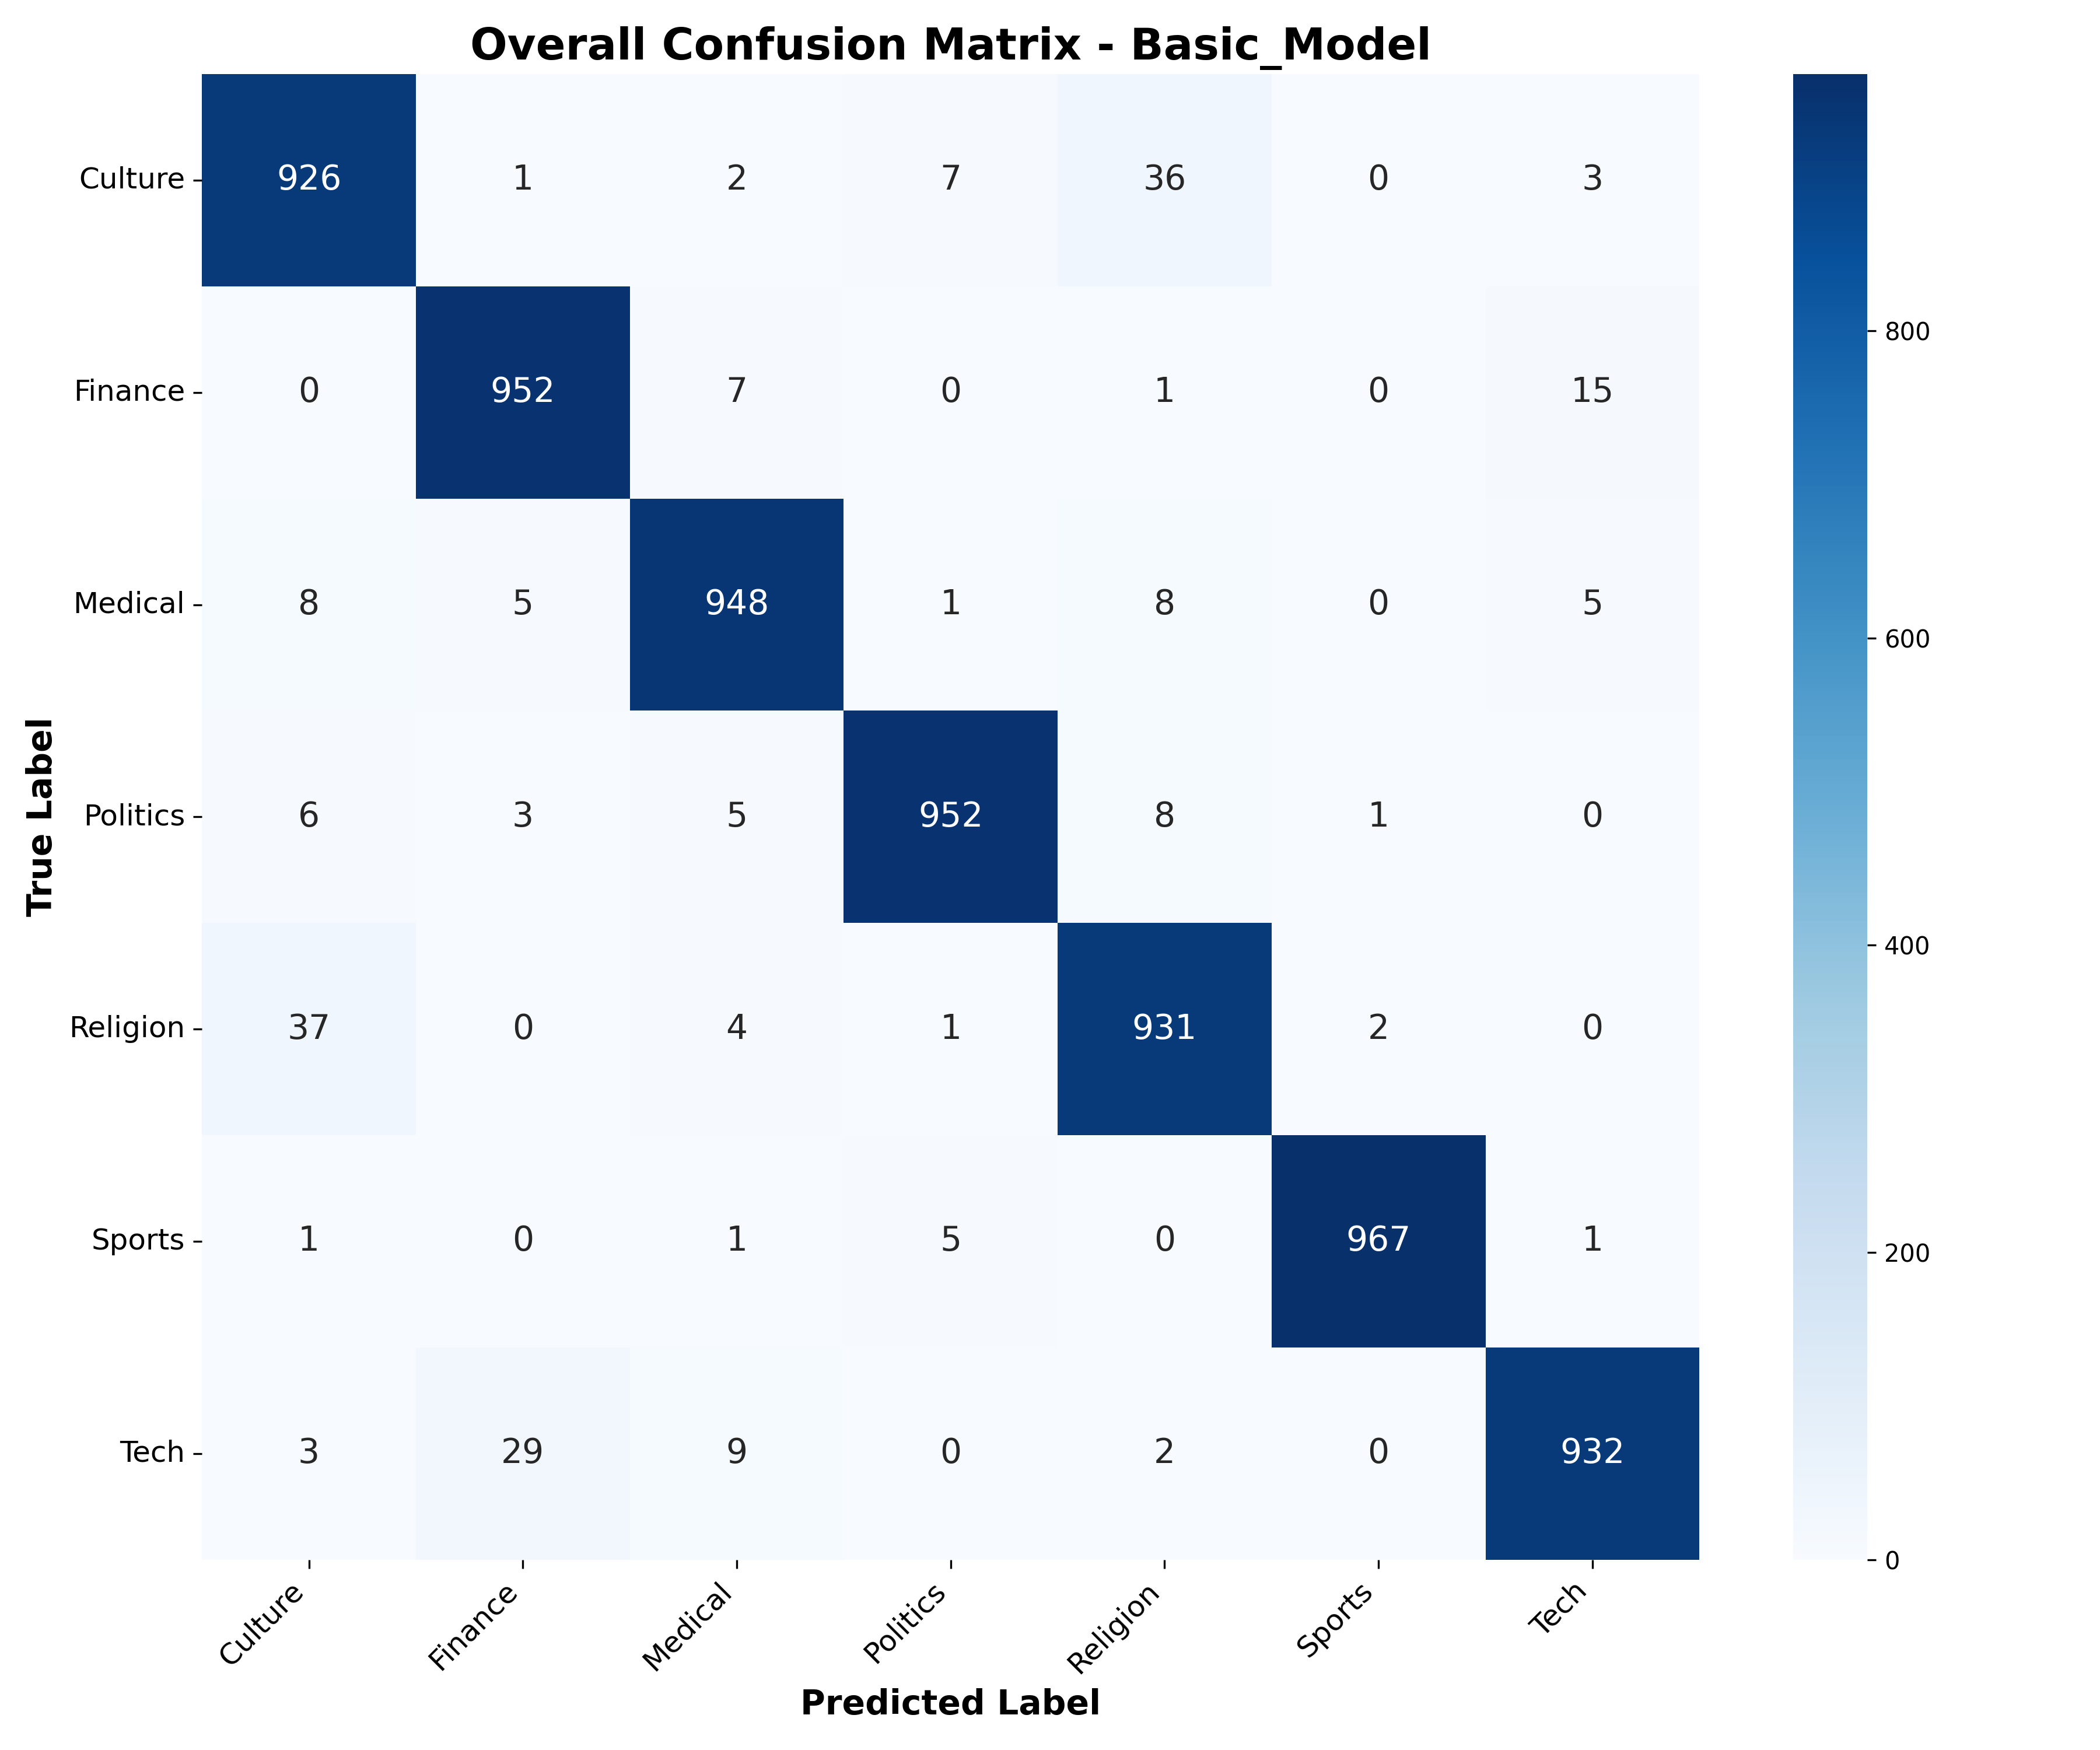
\includegraphics[width=0.9\textwidth]{Figures/confusion_matrices_Basic_Model/overall_confusion_matrix.png}
%DIFDELCMD < \caption{Overall confusion matrix for BERT Dense Head model across all seven news categories.}
%DIFDELCMD < \label{fig:cm_dense_overall}
%DIFDELCMD < \end{figure}
%DIFDELCMD < 

%DIFDELCMD < \begin{figure}[!ht]
%DIFDELCMD < \centering
%DIFDELCMD < 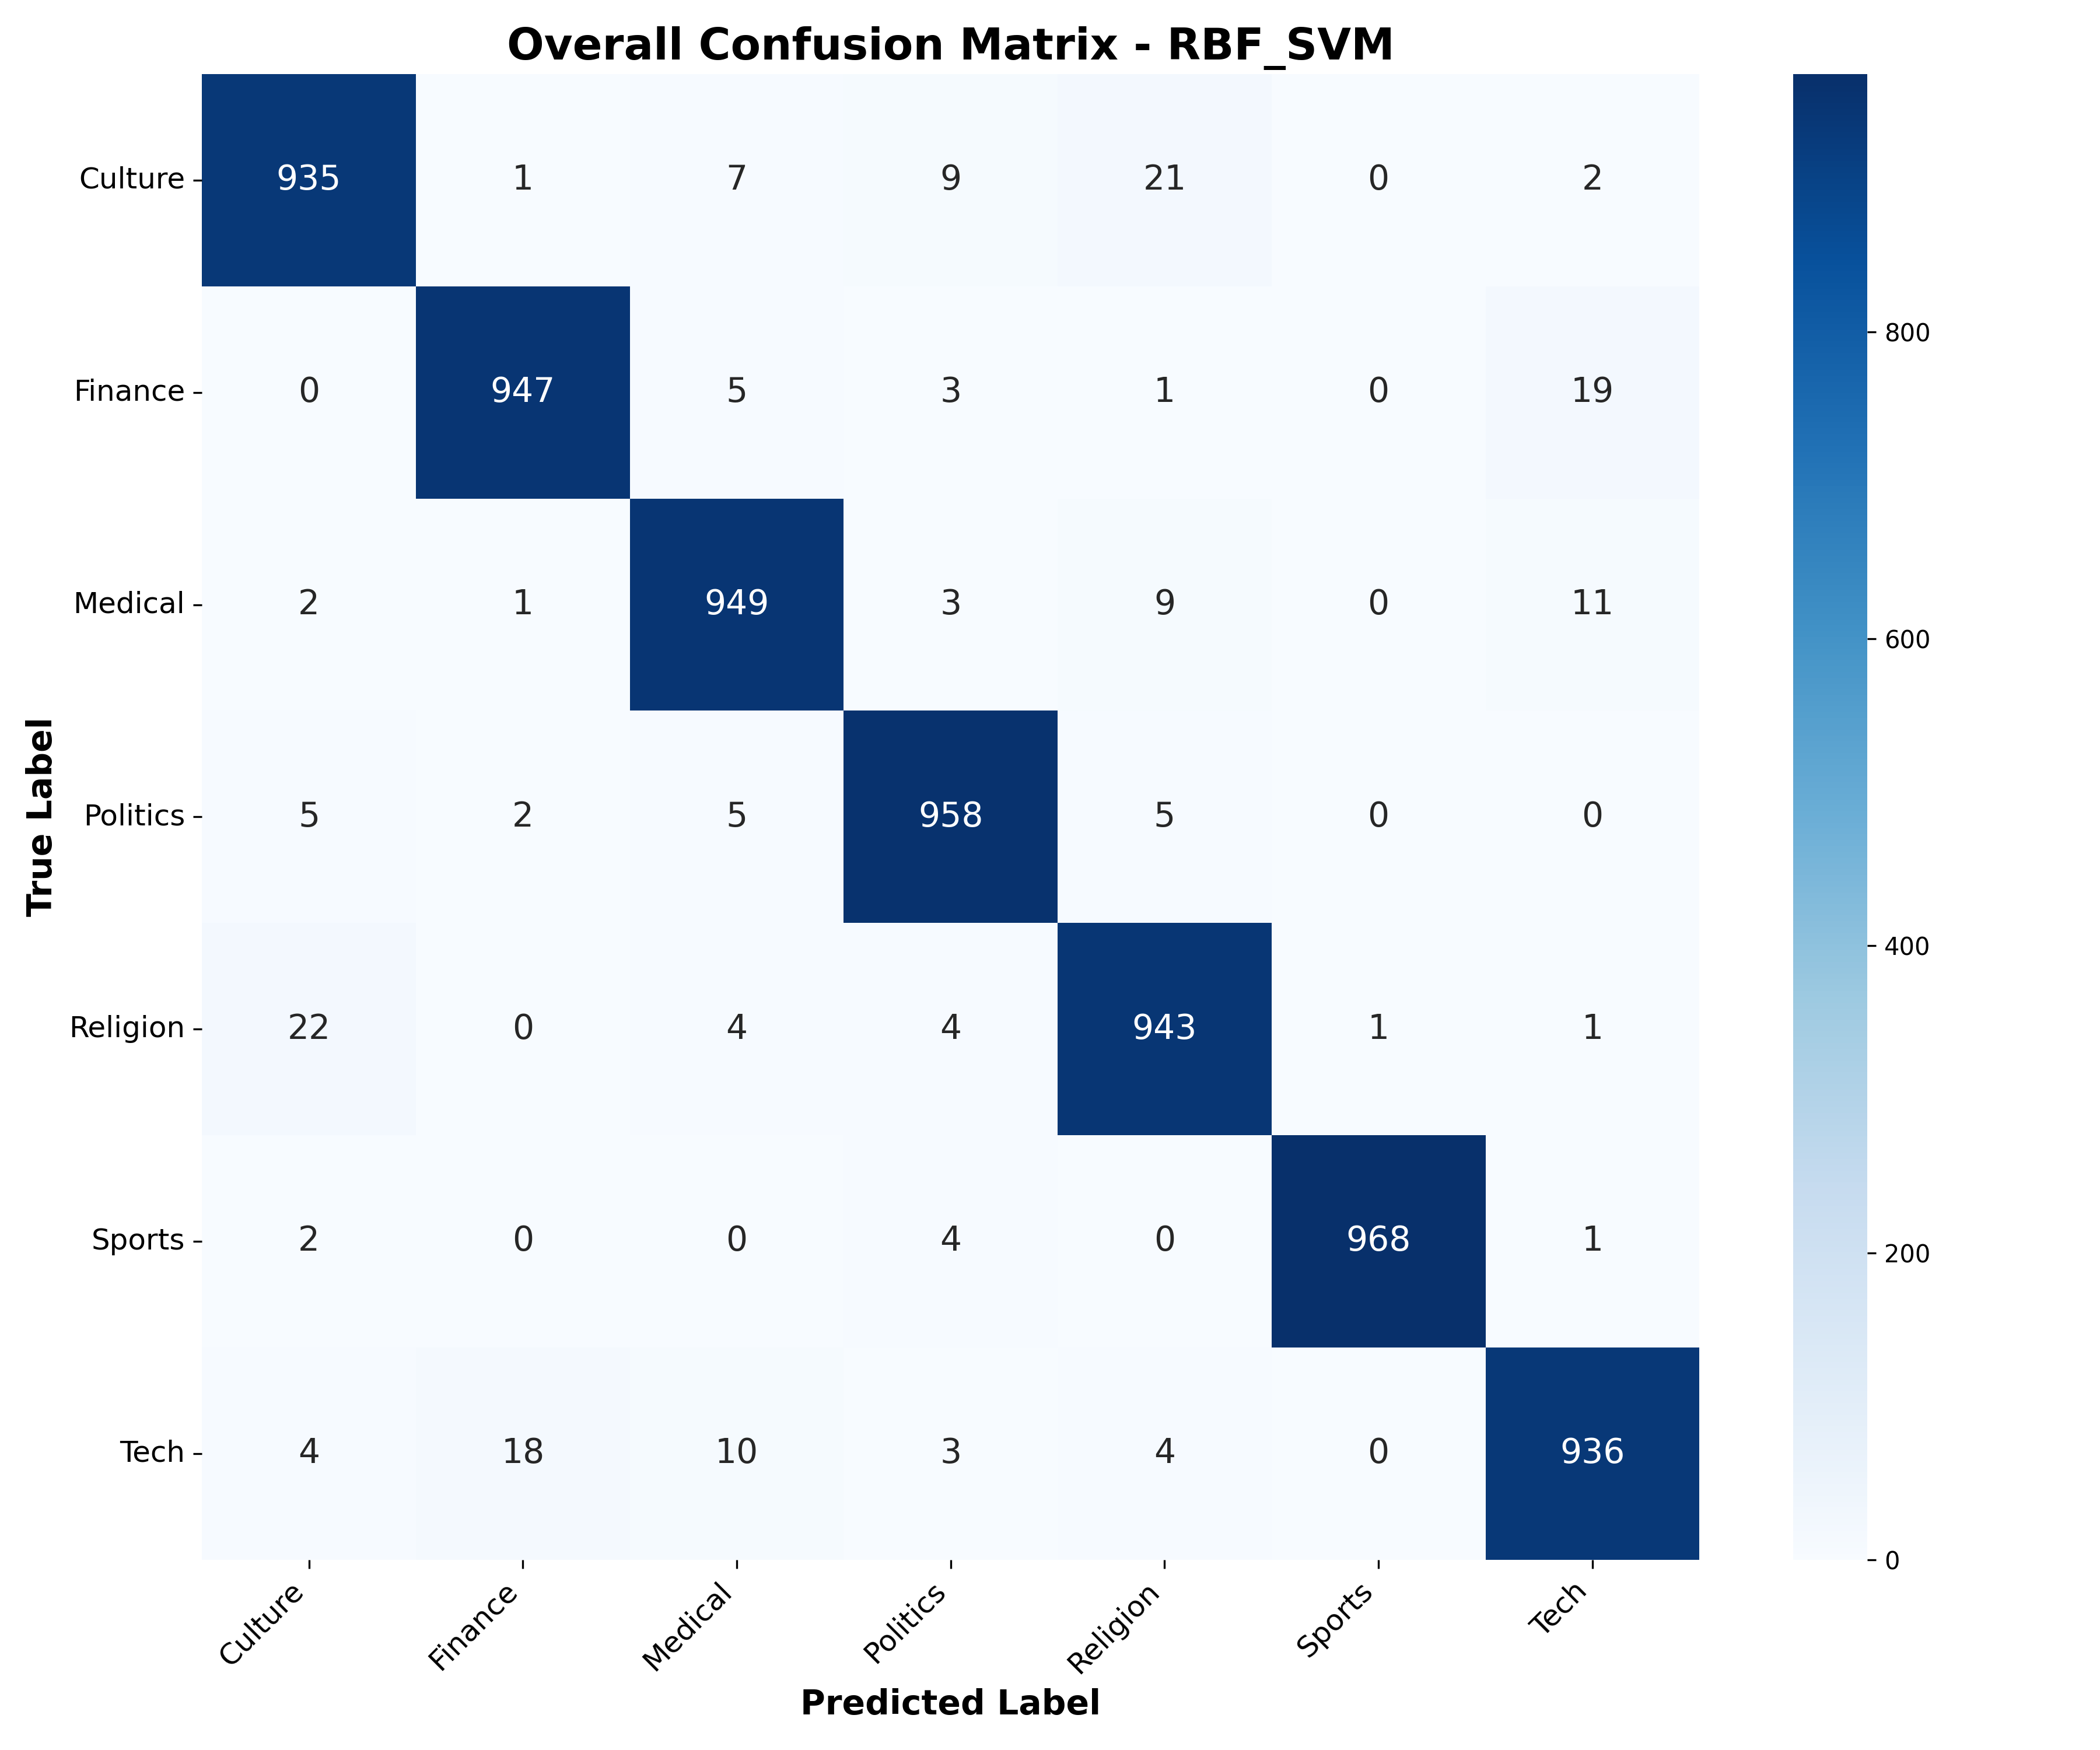
\includegraphics[width=0.9\textwidth]{Figures/confusion_matrices_RBF_SVM/overall_confusion_matrix.png}
%DIFDELCMD < \caption{Overall confusion matrix for BERT SVM Head model across all seven news categories.}
%DIFDELCMD < \label{fig:cm_svm_overall}
%DIFDELCMD < \end{figure}
%DIFDELCMD < 

%DIFDELCMD < %%%
\DIFdel{The confusion matrices reveal several important insights. Both BERT models demonstrate exceptional performance on }\textit{\DIFdel{Sports}} %DIFAUXCMD
\DIFdel{(967--968 correct out of 975 samples) }\DIFdelend \DIFaddbegin \DIFadd{recall of all systems. The two families err in different places. The supervised head's residual errors are spread thinly, with the two largest cells }\textit{\DIFadd{Religion}}\DIFadd{$\to$}\textit{\DIFadd{Culture}} \DIFadd{(44 of 973) }\DIFaddend and \DIFaddbegin \textit{\DIFadd{Tech}}\DIFadd{$\to$}\DIFaddend \textit{Finance} (\DIFdelbegin \DIFdel{947--952 correct out of }\DIFdelend \DIFaddbegin \DIFadd{28 of }\DIFaddend 975\DIFdelbegin \DIFdel{samples), achieving precision and recall above 0.97. In contrast, }\textit{\DIFdel{Culture}} %DIFAUXCMD
\DIFdel{and }\DIFdelend \DIFaddbegin \DIFadd{); full fine-tuning removes most of them (}\DIFaddend \textit{Religion} \DIFdelbegin \DIFdel{exhibit higher confusion rates, with 37--49 misclassifications in the Dense Head and 22--40 in the SVM Head. This pattern directly relates to the challenge faced by }\DIFdelend \DIFaddbegin \DIFadd{recall 0.99). The }\DIFaddend zero-shot \DIFdelbegin \DIFdel{LLMs: categories with overlapping linguistic features and similar formal registers require domain-specific fine-tuning to distinguish effectively.
}%DIFDELCMD < 

%DIFDELCMD < %%%
\DIFdel{The per-class confusion matrices illuminate why general-purpose LLMs struggle with certain categories while excelling in others. }\DIFdelend \DIFaddbegin \DIFadd{LLMs are at or above the supervised systems on }\textit{\DIFadd{Culture}}\DIFadd{, }\textit{\DIFadd{Finance}} \DIFadd{and }\DIFaddend \textit{Sports} \DIFdelbegin \DIFdel{maintains clear lexical boundaries (team names, player references, competition terminology) that even zero-shot models can identify reliably. However, categories like }\textit{\DIFdel{Religion}}%DIFAUXCMD
\DIFdel{, }\textit{\DIFdel{Culture}}%DIFAUXCMD
\DIFdel{, and }%DIFDELCMD < \textit{%%%
\DIFdel{Politics}%DIFDELCMD < \MBLOCKRIGHTBRACE %%%
\DIFdel{share overlapping vocabulary and similar syntactic structures in Gulf Arabic journalism. }%DIFDELCMD < 

%DIFDELCMD < %%%
\DIFdel{The BERT Dense Head confused 37 }\textit{\DIFdel{Religion}} %DIFAUXCMD
\DIFdel{samples as }\textit{\DIFdel{Culture}} %DIFAUXCMD
\DIFdel{and 36 }\textit{\DIFdel{Culture}} %DIFAUXCMD
\DIFdel{samples as }\textit{\DIFdel{Religion}}%DIFAUXCMD
\DIFdel{, revealing the fundamental challenge: both categories use formal MSA register, reference institutional authorities, and discuss social values. Without exposure to thousands of labeled examples distinguishing these categories, LLMs rely on surface-level heuristics that fail when contextual understanding is required. For instance, an article about a religious leader\'s comments on social issues could legitimately be classified as either }\textit{\DIFdel{Religion}} %DIFAUXCMD
\DIFdel{or }\DIFdelend \DIFaddbegin \DIFadd{but lose 4--13 points on }\textit{\DIFadd{Medical}}\DIFadd{, }\DIFaddend \textit{Politics} \DIFdelbegin \DIFdel{depending on framing---a nuance that fine-tuned models learn through training data patterns but zero-shot LLMs must infer from ambiguous prompts. }%DIFDELCMD < 

%DIFDELCMD < %%%
\DIFdel{The confusion between }\DIFdelend \DIFaddbegin \DIFadd{and }\DIFaddend \textit{Tech}\DIFaddbegin \DIFadd{, and 20--25 points on }\textit{\DIFadd{Religion}}\DIFadd{, where GPT-4.1 routes 172 of 973 articles to }\textit{\DIFadd{Culture}} \DIFadd{and smaller numbers to }\textit{\DIFadd{Medical}} \DIFaddend and \DIFdelbegin \textit{\DIFdel{Finance}} %DIFAUXCMD
\DIFdelend \DIFaddbegin \textit{\DIFadd{Politics}}\DIFadd{. The pattern is the same for all four API models }\DIFaddend (\DIFdelbegin \DIFdel{29 misclassifications in Dense Head, 18 in SVM Head) reflects another common LLM failure mode. Technology companies in Gulf news are often discussed in economic contexts---investments, valuations, market strategies---creating lexical overlap that misleads models without domain-specific training. The SVM Head\'s improvement over Dense Head in this distinction (reducing Tech$\rightarrow$Finance errors from 29 to 18) suggests that linear decision boundaries in the embedding space can effectively separate these categories once the encoder is properly fine-tuned, whereas LLMs processing raw text struggle with this ambiguity.
}%DIFDELCMD < 

%DIFDELCMD < %%%
\DIFdel{Table~\ref{tab:per_class_performance} presents the detailed per-class metrics for both BERT models, computed from the confusion matrices. The }\textit{\DIFdel{Sports}} %DIFAUXCMD
\DIFdel{category shows the most consistent results, with fine-tuned BERT models achieving near-perfect precision (0.99--1.00) and recall (0.99) . The }\DIFdelend \textit{Religion} \DIFdelbegin \DIFdel{category, while still performing well in BERT models (precision0.94}\DIFdelend \DIFaddbegin \DIFadd{recall 0.71}\DIFaddend --0\DIFdelbegin \DIFdel{.96, recall 0.95--0.97), shows notably more confusion with }\textit{\DIFdel{Culture}} %DIFAUXCMD
\DIFdel{and }\textit{\DIFdel{Politics}}%DIFAUXCMD
\DIFdel{. This explains why Claude-3}\DIFdelend \DIFaddbegin \DIFadd{.76) and more pronounced for Qwen2}\DIFaddend .5\DIFdelbegin \DIFdel{-Haiku completely failed on }\textit{\DIFdel{Religion}} %DIFAUXCMD
\DIFdel{(recall = 0): without fine-tuning, the model cannot distinguish the subtle contextual cues that separate religious institutional announcements from cultural or political discourse with religious references. }%DIFDELCMD < 

%DIFDELCMD < \begin{table}[!ht]
%DIFDELCMD < \centering
%DIFDELCMD < \caption{Per-Class Performance Metrics for BERT Models}
%DIFDELCMD < \label{tab:per_class_performance}
%DIFDELCMD < \small
%DIFDELCMD < \begin{tabular}{lcccccc}
%DIFDELCMD < \hline
%DIFDELCMD < \textbf{Category} & \multicolumn{3}{c}{\textbf{BERT Dense Head}} & \multicolumn{3}{c}{\textbf{BERT SVM Head}} \\
%DIFDELCMD < \cline{2-4} \cline{5-7}
%DIFDELCMD <  & \textbf{Precision} & \textbf{Recall} & \textbf{F1} & \textbf{Precision} & \textbf{Recall} & \textbf{F1} \\
%DIFDELCMD < \hline
%DIFDELCMD < Culture & 0.95 & 0.95 & 0.95 & 0.96 & 0.96 & 0.96 \\
%DIFDELCMD < Finance & 0.96 & 0.98 & 0.97 & 0.98 & 0.97 & 0.97 \\
%DIFDELCMD < Medical & 0.97 & 0.97 & 0.97 & 0.97 & 0.97 & 0.97 \\
%DIFDELCMD < Politics & 0.97 & 0.98 & 0.97 & 0.98 & 0.98 & 0.98 \\
%DIFDELCMD < Religion & 0.94 & 0.95 & 0.95 & 0.96 & 0.97 & 0.96 \\
%DIFDELCMD < Sports & 0.99 & 0.99 & 0.99 & 1.00 & 0.99 & 1.00 \\
%DIFDELCMD < Tech & 0.97 & 0.96 & 0.96 & 0.96 & 0.96 & 0.96 \\
%DIFDELCMD < \hline
%DIFDELCMD < \end{tabular}
%DIFDELCMD < \end{table}
%DIFDELCMD < 

%DIFDELCMD < %%%
\subsection{\DIFdel{Training and Inference Efficiency}}
%DIFAUXCMD
\addtocounter{subsection}{-1}%DIFAUXCMD
\DIFdel{Figures~\ref{fig:train_time} and~\ref{fig:test_time} compare the supervised models. The BERT--SVM head trained in 4.38 seconds, 58.4\% faster than the Dense Head (10.54 seconds) }\DIFdelend \DIFaddbegin \DIFadd{-7B (0.53), so it is a property of the task framing rather than of one model. The articles involved are typically historical or devotional pieces that the publisher files under }\textit{\DIFadd{Religion}} \DIFadd{and that a general-purpose model can defensibly read as cultural; the supervised systems learn this publisher-specific convention from the labels, which the LLMs cannot know}\DIFaddend .
\DIFdelbegin \DIFdel{However, inference was slightly faster for the Dense Head, making it more suitable for latency-sensitive deployment. Both models produced sub-second inference times, validating their feasibility for real-time tasks. Timing data for zero-shot LLMs were excluded, as latency was dominated by provider-side variability.
}\DIFdelend 

\DIFdelbegin %DIFDELCMD < \begin{figure}[H]
%DIFDELCMD < \centering
%DIFDELCMD < 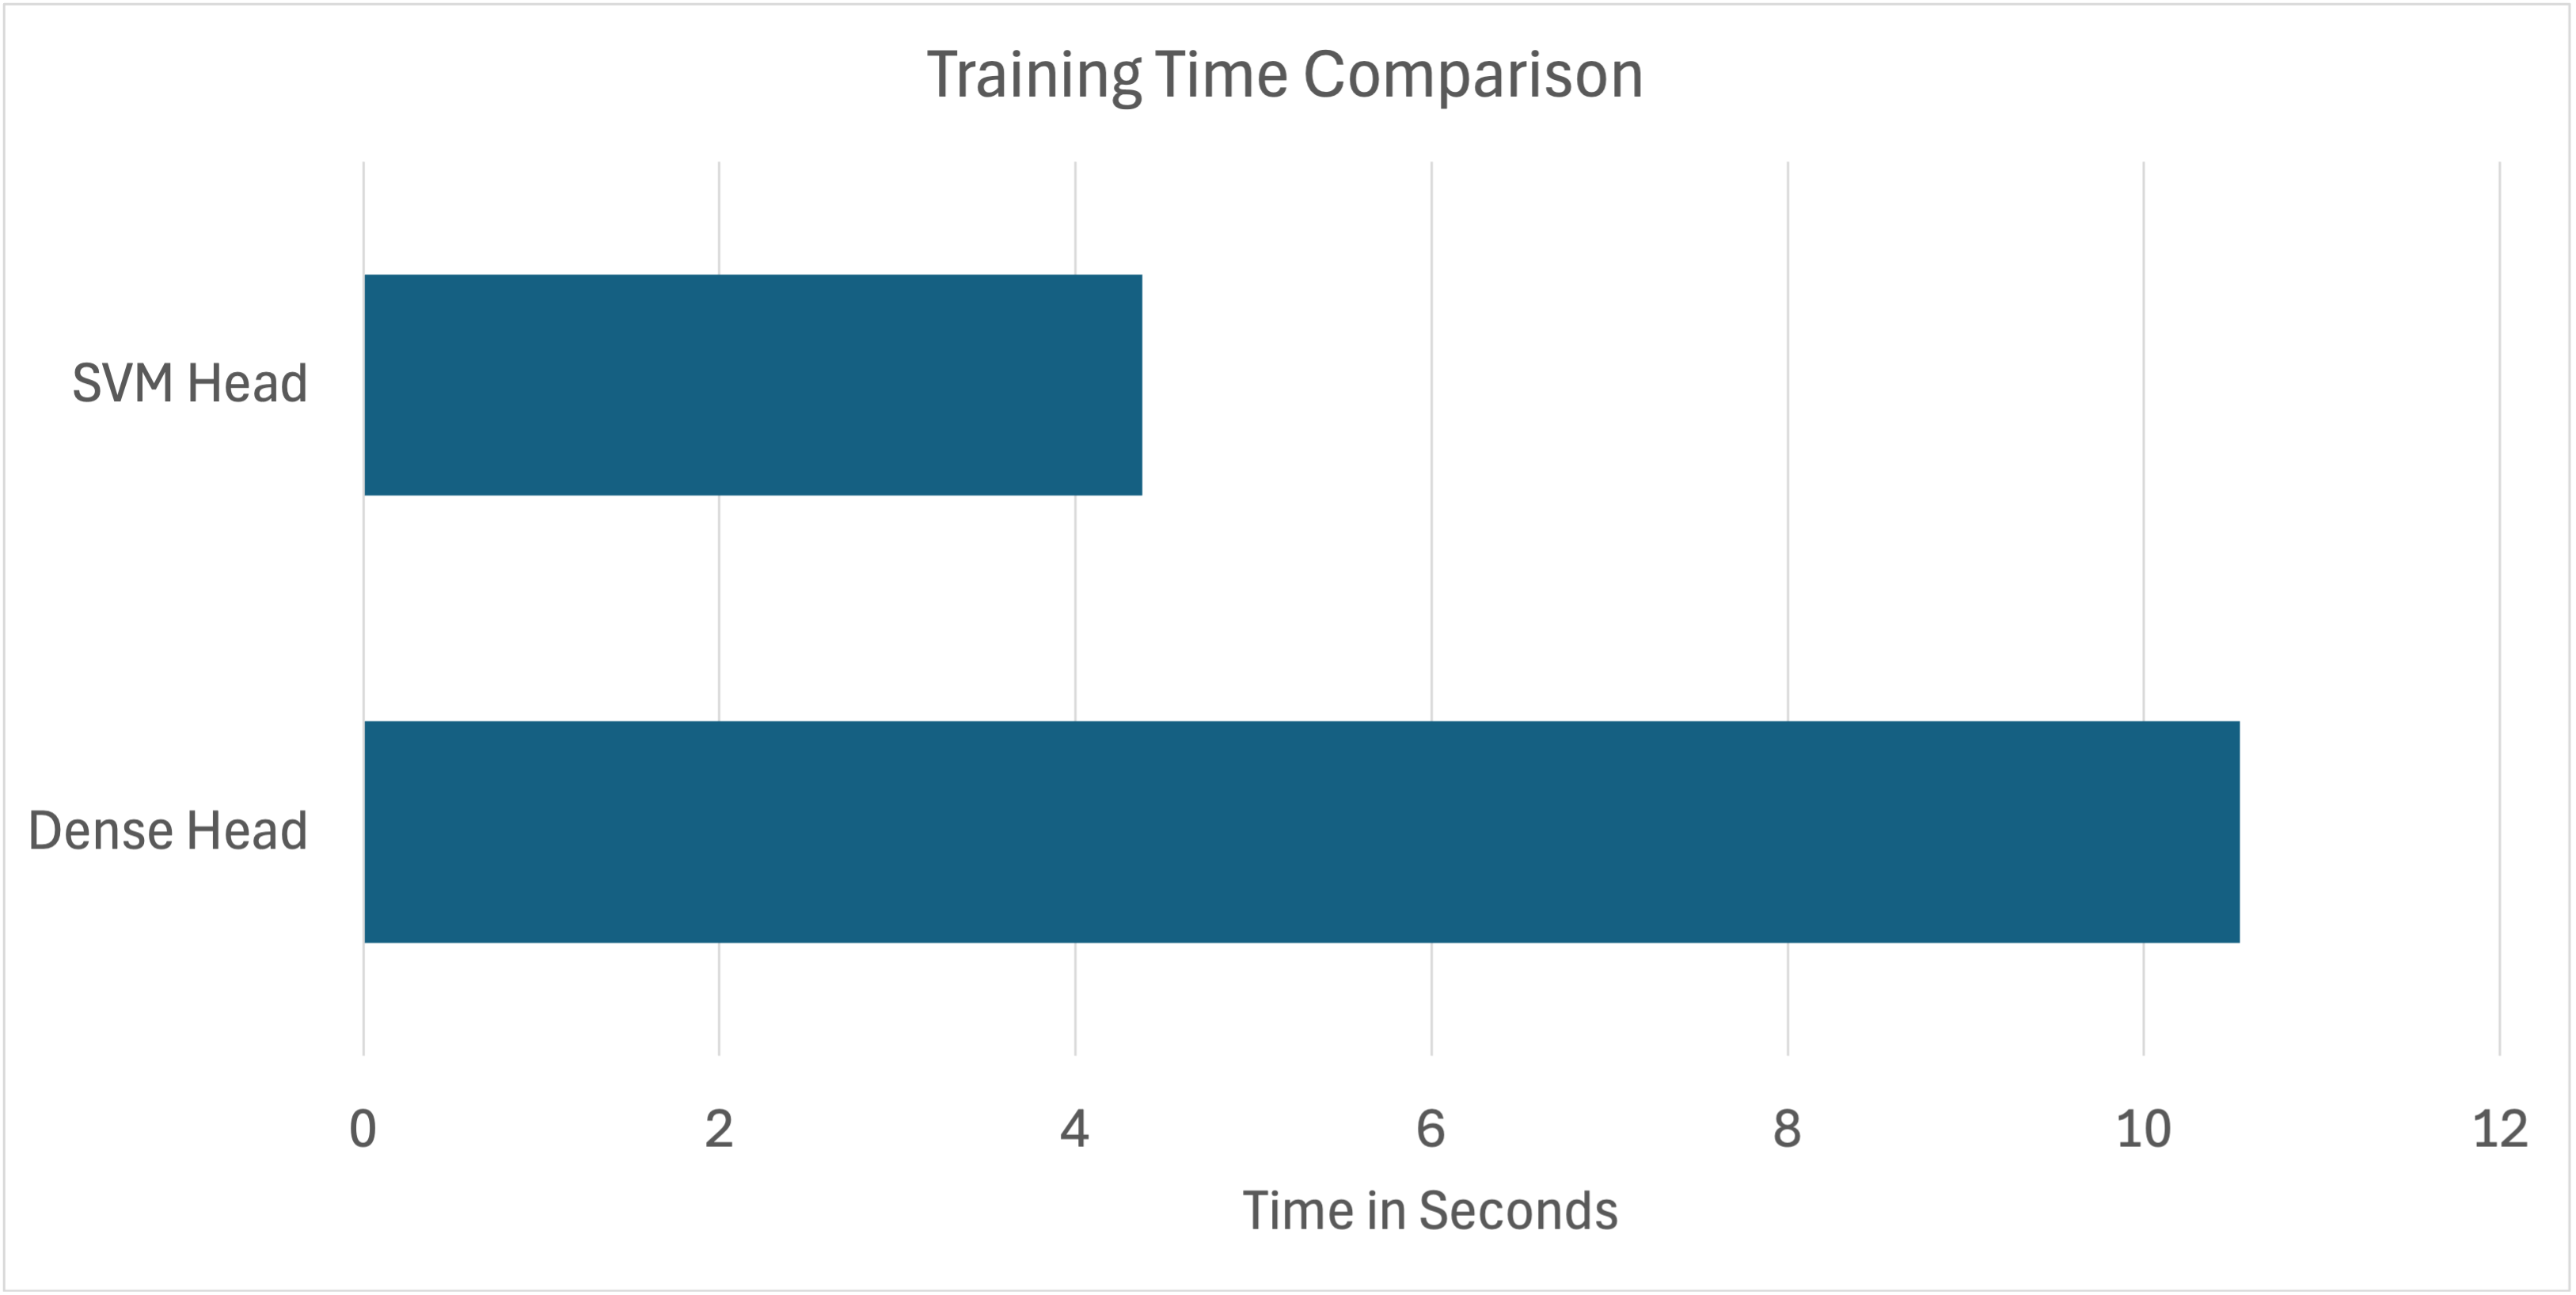
\includegraphics[width=0.9\textwidth]{Figures/Train_time.png}
%DIFDELCMD < \caption{Training time comparison between BERT Dense Head and BERT SVM Head models.}
%DIFDELCMD < \label{fig:train_time}
%DIFDELCMD < \end{figure}
%DIFDELCMD < %%%
\DIFdelend \DIFaddbegin \begin{figure}[!ht]
\centering
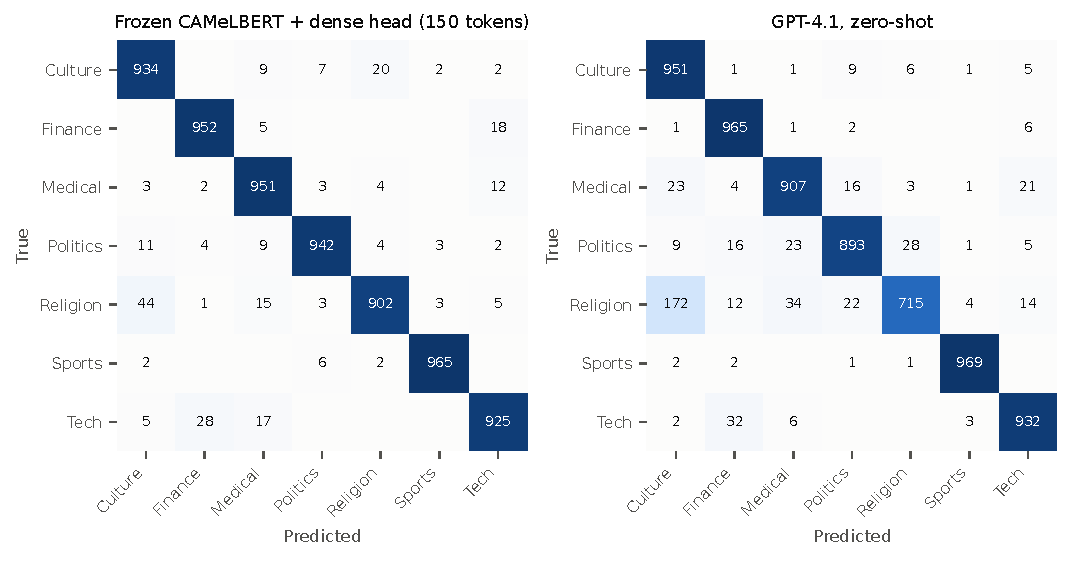
\includegraphics[width=\textwidth]{fig_confusion.pdf}
\caption{Confusion matrices on the shared test split (rows: true class; columns: predicted class; counts). Left: frozen CAMeLBERT with the dense head (150 wordpieces, seed 0). Right: GPT-4.1 zero-shot with the primary prompt.}
\label{fig:confusion}
\end{figure}
\DIFaddend 

\DIFdelbegin %DIFDELCMD < \begin{figure}[H]
%DIFDELCMD < \centering
%DIFDELCMD < 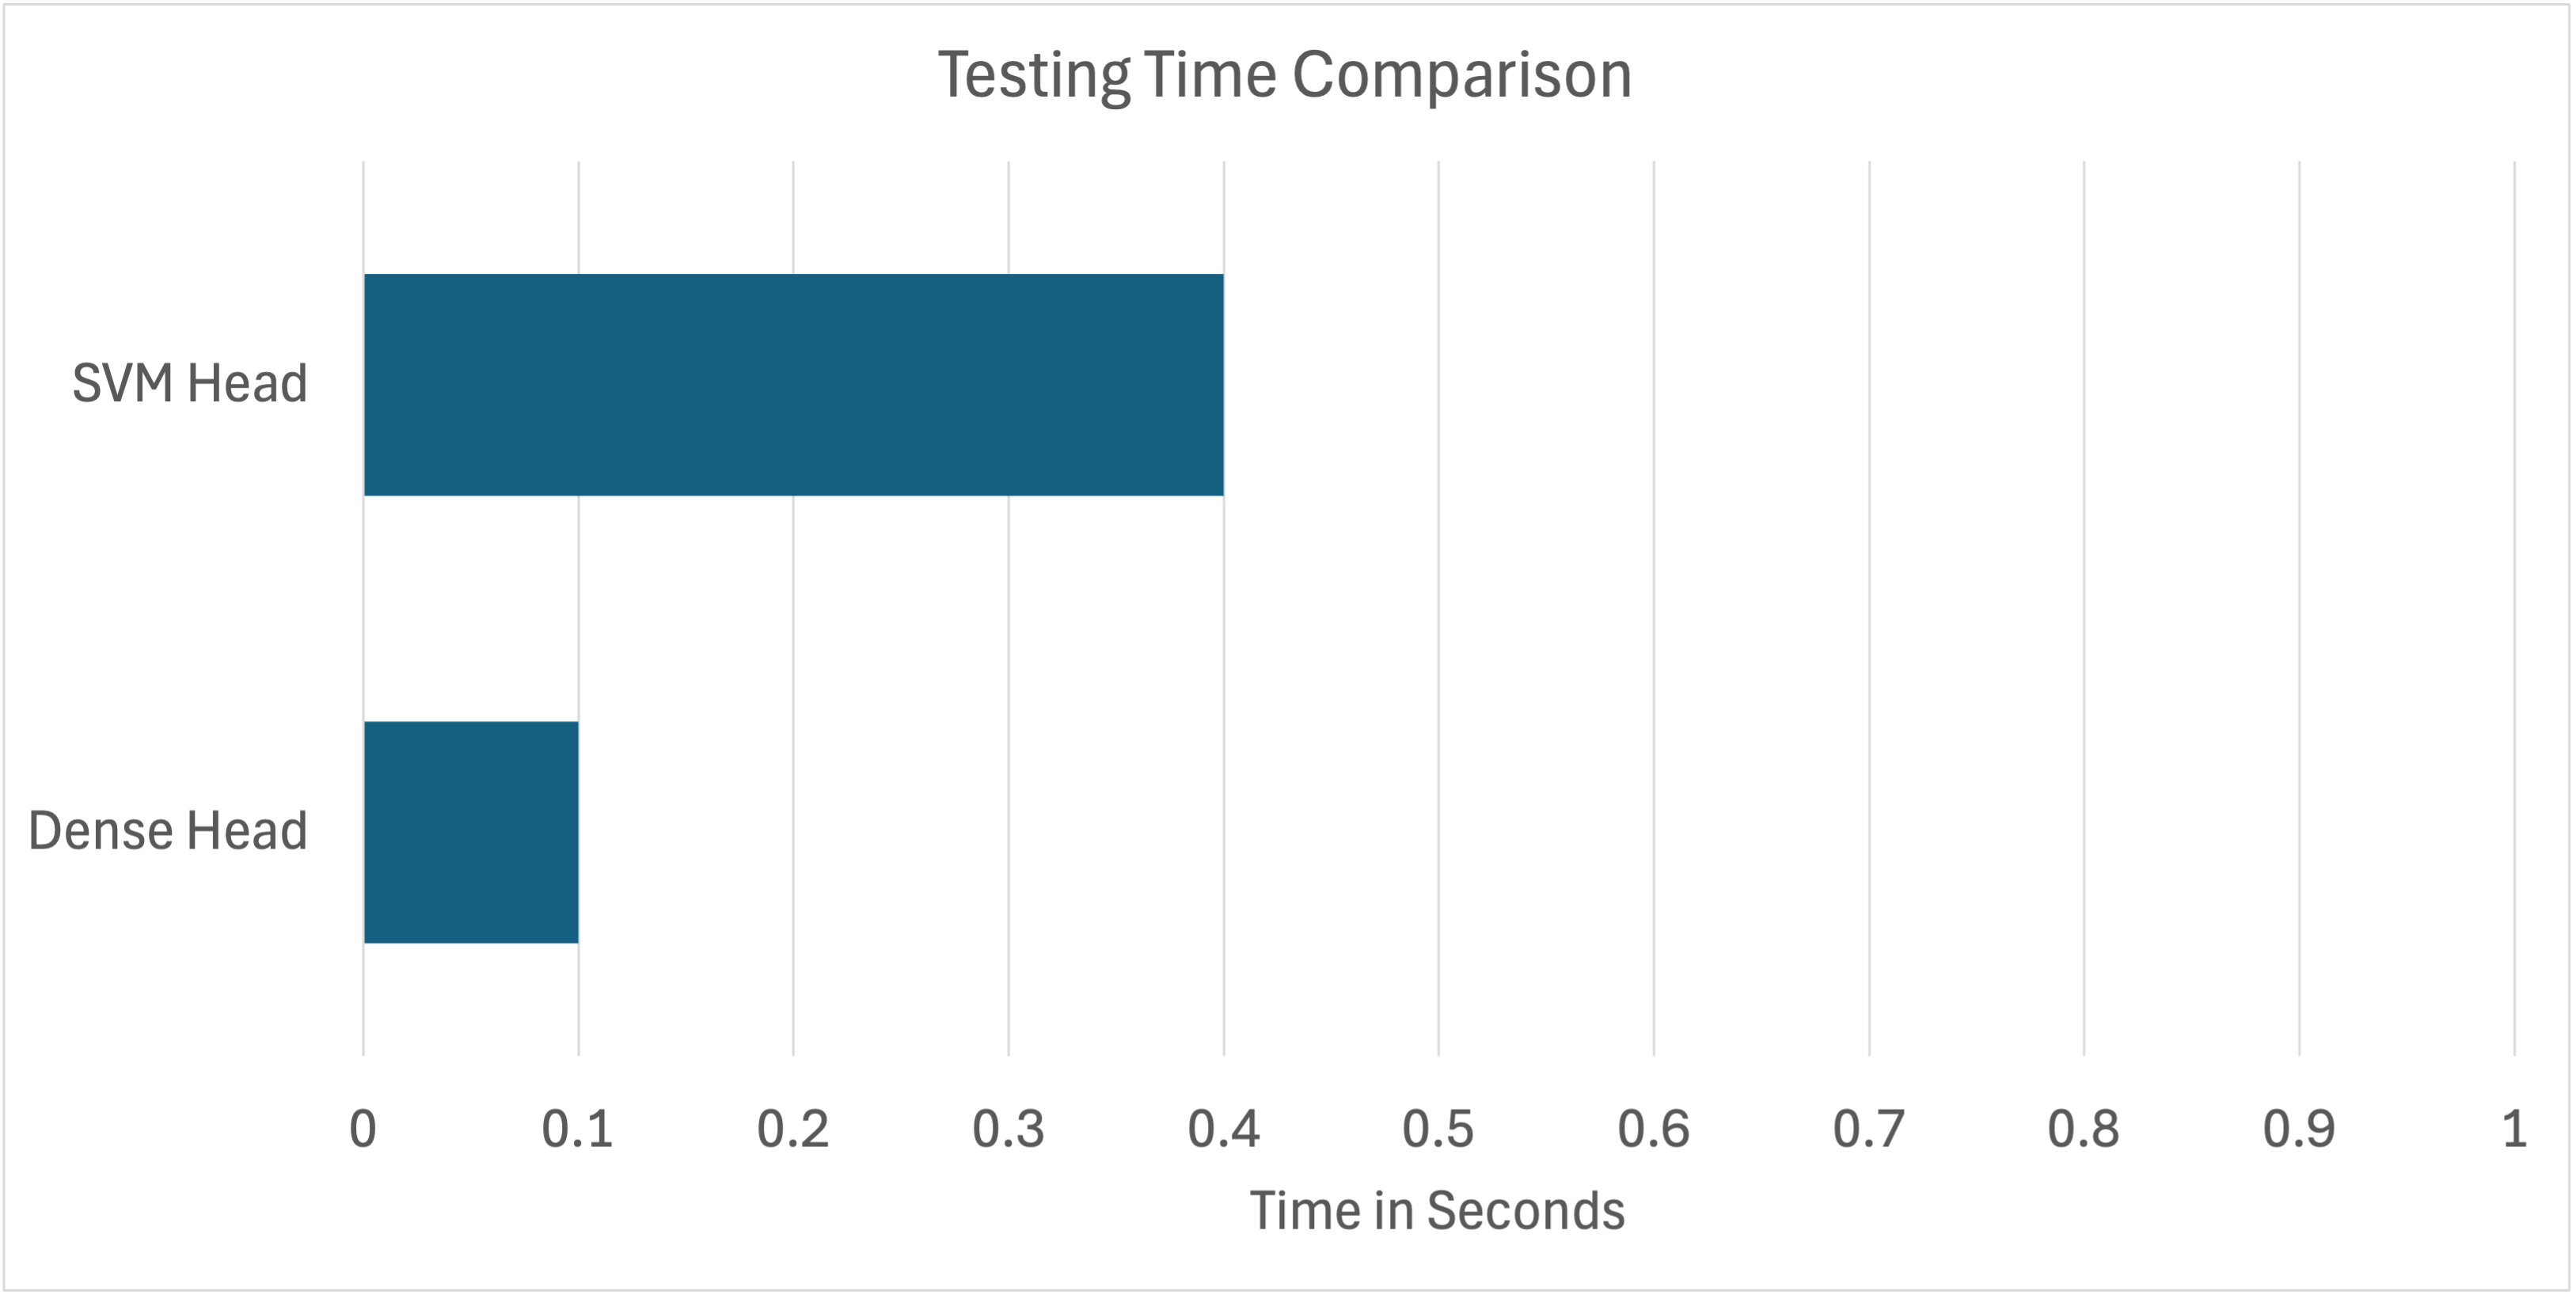
\includegraphics[width=0.9\textwidth]{Figures/Test_time.png}
%DIFDELCMD < \caption{Inference time comparison between BERT Dense Head and BERT SVM Head models.}
%DIFDELCMD < \label{fig:test_time}
%DIFDELCMD < \end{figure}
%DIFDELCMD < %%%
\DIFdelend \DIFaddbegin \begin{table}[!ht]
\centering
\caption{Per-class recall on the shared test split (975 articles per class, 973--977 after deduplication). Supervised systems: mean over seeds; LLMs: zero-shot, primary prompt. Religion is the weakest class for every zero-shot LLM and the only class where the gap to the supervised systems exceeds 20 points.}
\label{tab:perclass}
\small
\resizebox{\ifdim\width>\textwidth\textwidth\else\width\fi}{!}{%
\begin{tabular}{@{}l rrrr rrrr@{}}
\toprule
 & \multicolumn{4}{c}{\textbf{Supervised / adapted}} & \multicolumn{4}{c}{\textbf{Zero-shot LLMs}} \\
\cmidrule(lr){2-5}\cmidrule(lr){6-9}
\textbf{Class} & Dense 150 & SVM 150 & Fine-tuned & QLoRA all & GPT-4.1 & Claude 4.5 & Gemini 3.8 & DeepSeek V4 \\
\midrule
Culture & 0.939 & 0.945 & 0.994 & 0.968 & 0.976 & 0.977 & 0.990 & 0.975 \\
Finance & 0.977 & 0.974 & 0.977 & 0.990 & 0.990 & 0.992 & 0.998 & 0.993 \\
Medical & 0.972 & 0.972 & 0.982 & 0.989 & 0.930 & 0.896 & 0.920 & 0.875 \\
Politics & 0.970 & 0.985 & 0.993 & 0.993 & 0.916 & 0.939 & 0.949 & 0.974 \\
Religion & 0.955 & 0.965 & 0.986 & 0.980 & 0.735 & 0.741 & 0.716 & 0.705 \\
Sports & 0.992 & 0.992 & 0.998 & 0.998 & 0.994 & 0.991 & 0.992 & 0.984 \\
Tech & 0.944 & 0.964 & 0.994 & 0.977 & 0.956 & 0.906 & 0.838 & 0.899 \\
\midrule
Macro F1 & 0.964 & 0.971 & 0.989 & 0.985 & 0.927 & 0.919 & 0.914 & 0.914 \\
\bottomrule
\end{tabular}}
\end{table}
\DIFaddend 


\DIFdelbegin \subsection{\DIFdel{Qualitative Error Analysis}}
%DIFAUXCMD
\addtocounter{subsection}{-1}%DIFAUXCMD
\DIFdelend \DIFaddbegin \subsection{\DIFadd{How Much Supervision Does the Lightweight System Need?}}
\label{sec:lc}
\DIFaddend 

\DIFdelbegin \DIFdel{Despite overall high performance, misclassifications provide insight into model limitations. Table~\ref{tab:model-evaluation} shows examples where the BERT Dense Head failed. Financial news with embedded numeric details was sometimes mislabeled as }\textit{\DIFdel{Sports}}%DIFAUXCMD
\DIFdel{, likely due to superficial lexical overlap. Similarly, medical-sector content was mislabeled as }\textit{\DIFdel{Religion}}%DIFAUXCMD
\DIFdel{, showing challenges in distinguishing domain-specific entities when contextual cues are weak}\DIFdelend \DIFaddbegin \DIFadd{Figure~\ref{fig:lc} and Table~\ref{tab:lc} report the learning curve. With 10 labelled articles per class the frozen dense head reaches 82.5\% (88.4\% at 512 wordpieces), with 50 per class 90.9\% (94.2\%), and with 100 per class 92.9\% (95.1\%), which already matches or exceeds the best zero-shot LLM (92.8\%)}\DIFaddend . \DIFdelbegin %DIFDELCMD < 

%DIFDELCMD < \begin{table}[h!]
%DIFDELCMD <     \centering
%DIFDELCMD <     \caption{Representative Misclassifications — BERT Dense Head}
%DIFDELCMD <     \label{tab:model-evaluation}
%DIFDELCMD <     \begin{tabularx}{\textwidth}{>{\raggedleft\arraybackslash}X c c c}
%DIFDELCMD <         \toprule
%DIFDELCMD <         \textbf{Text} & \textbf{Model Output} & \textbf{Original Output} & \textbf{Result} \\
%DIFDELCMD <         \midrule
%DIFDELCMD <         \RTL{دبي "الخليج" : أعلنت شركة "غلفا للمياه المعدنية" أنها حققت أرباحاً بلغت مليون درهم في 2015 مقارنة مع 6.4 مليون درهم في 2014، بعد خصم أعباء حقوق حكومة عجمان البالغة مليوني درهم، وتراجعت المبيعات إلى 7 ملايين كرتونة في 2015 مقابل 7.9 مليون كرتونة في 2014.} &
%DIFDELCMD <         Sports & Finance & miss \\
%DIFDELCMD <         \addlinespace
%DIFDELCMD <         \RTL{دبي: "الخليج" استقبل خلف أحمد الحبتور، مؤسس ورئيس مجلس إدارة مجموعة الحبتور، الدكتور ستيفن فيكتور، الرئيس التنفيذي والمدير الطبي لدى "ريجين مديكال" في دبي.} &
%DIFDELCMD <         Religion & Medical & miss \\
%DIFDELCMD <         \bottomrule
%DIFDELCMD <     \end{tabularx}
%DIFDELCMD < \end{table}
%DIFDELCMD < 

%DIFDELCMD < %%%
\DIFdelend The \DIFdelbegin \DIFdel{SVM-based model produced different error patterns (Table~\ref{tab:model-svm-evaluation}) . It often mislabeled }%DIFDELCMD < \textit{%%%
\DIFdel{Technology}%DIFDELCMD < \MBLOCKRIGHTBRACE %%%
\DIFdel{news as }\textit{\DIFdel{Finance}}%DIFAUXCMD
\DIFdelend \DIFaddbegin \DIFadd{few-shot conditions were measured on the 700-article subset, so we compare them with the supervised systems scored on the same 700 articles: at 500 per class the 512-wordpiece head reaches 96.7\% there against 95.3\% for the best few-shot condition (Gemini 3.8 Flash, $k=2$), whereas the 150-wordpiece head (94.4\% at 500 and 95.0\% at 1,000 per class) only passes it with the full training split (96.5\%; the RBF-SVM does so from 1}\DIFaddend ,\DIFdelbegin \DIFdel{suggesting an over-reliance on economic keywords. This points to a sensitivity to surface-level tokens without capturing deeper semantic relationships. }%DIFDELCMD < 

%DIFDELCMD < \begin{table}[h!]
%DIFDELCMD <     \centering
%DIFDELCMD <     \caption{Representative Misclassifications — BERT SVM Head}
%DIFDELCMD <     \label{tab:model-svm-evaluation}
%DIFDELCMD <     \begin{tabularx}{\textwidth}{>{\raggedleft\arraybackslash}X c c c}
%DIFDELCMD <         \toprule
%DIFDELCMD <         \textbf{Text} & \textbf{Model Output} & \textbf{Original Output} & \textbf{Result} \\
%DIFDELCMD <         \midrule
%DIFDELCMD <         \RTL{دبي: محمد إبراهيم أطلقت وزارة التربية والتعليم خلال مشاركتها في "أسبوع جيتكس للتقنية" خدمتين جديدتين تضافان إلى خدماتها الذكية الأخرى.} &
%DIFDELCMD <         Finance & Tech & miss \\
%DIFDELCMD <         \addlinespace
%DIFDELCMD <         \RTL{دبي: "الخليج" أعلنت شركة "إل جي" أنها ستوفر أحدث الحلول التفاعلية الرقمية في دبي باركس آند ريزورتس، أكبر منتجع سياحي وترفيهي في المنطقة.} &
%DIFDELCMD <         Finance & Tech & miss \\
%DIFDELCMD <         \bottomrule
%DIFDELCMD <     \end{tabularx}
%DIFDELCMD < \end{table}
%DIFDELCMD < 

%DIFDELCMD < %%%
\DIFdel{To provide a comprehensive understanding of model behavior, this section presents systematic qualitative analysis organized into three categories: (}\DIFdelend \DIFaddbegin \DIFadd{000 per class, 95.7\%). On the full test set the curves continue to rise to 96.4\% / 97.5\% with the full split. The RBF-SVM follows the same curve within one point. Full fine-tuning and QLoRA start higher and saturate earlier: 96.6\% and 95.7\% with 100 per class, 98.4\% for both with }\DIFaddend 1\DIFdelbegin \DIFdel{) examples where all models correctly classify the text, (2) instances where the proposed BERT models succeed while }\DIFdelend \DIFaddbegin \DIFadd{,000 per class, and 98.9\% and 98.5\% with the full split. In other words, the crossover between }\DIFaddend zero-shot \DIFdelbegin \DIFdel{LLMs fail, and (3)cases where LLMs correctly predict the label while BERT models err. This analysis reveals the complementary strengths and distinct failure modes of supervised and zero-shot approaches}\DIFdelend \DIFaddbegin \DIFadd{LLM inference and in-domain supervision on this task lies at roughly 100 labelled articles per class for a 0.3\,M-parameter head, and the ceiling of the task is reached with about 1,000 per class by any adapted model}\DIFaddend .

\DIFdelbegin \subsubsection{\DIFdel{Correctly Classified Examples}}
%DIFAUXCMD
\addtocounter{subsubsection}{-1}%DIFAUXCMD
\DIFdelend \DIFaddbegin \begin{figure}[!ht]
\centering
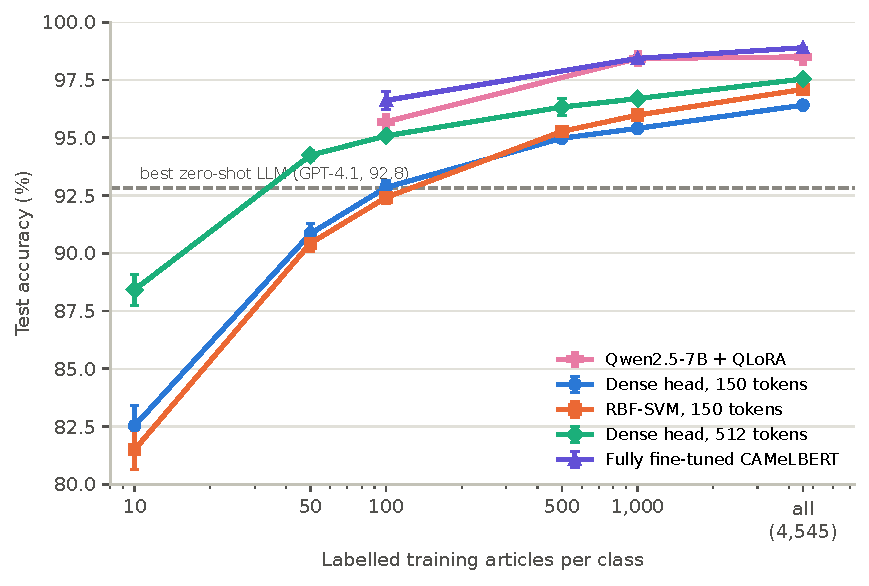
\includegraphics[width=0.9\textwidth]{fig_learning_curve.pdf}
\caption{Learning curve on the shared test split: accuracy as a function of labelled training articles per class (log scale; mean and standard deviation over three seeds; nested subsets). The horizontal line marks the best zero-shot LLM on the full test set; the few-shot conditions were measured on the 700-article subset and are compared with the supervised systems on that subset in the text.}
\label{fig:lc}
\end{figure}
\DIFaddend 

\DIFdelbegin \DIFdel{Table~\ref{tab:correct-examples} presents representative examples where both BERT architectures and all zero-shot LLMs achieved correct classifications. These examples illustrate the characteristics of unambiguous news articles that models handle reliably. }\DIFdelend \DIFaddbegin \begin{table}[!ht]
\centering
\caption{Learning curve: test accuracy (\%) as a function of the number of labelled training articles per class (mean $\pm$ standard deviation over three seeds; ``all'' = the full training split, about 4{,}545 per class). Nested subsets drawn with a fixed ranking of the training split. For reference, the best zero-shot LLM reaches 92.8\,\% on the full test set; the best few-shot condition, 95.3\,\% (Table~\ref{tab:prompts}), was measured on the 700-article subset and is compared with the supervised systems on that subset in the text.}
\label{tab:lc}
\small
\resizebox{\ifdim\width>\textwidth\textwidth\else\width\fi}{!}{%
\begin{tabular}{@{}l rrrrrr@{}}
\toprule
\textbf{System} & \textbf{10} & \textbf{50} & \textbf{100} & \textbf{500} & \textbf{1{,}000} & \textbf{all} \\
\midrule
Dense head, 150 tokens & 82.5$\pm$0.9 & 90.9$\pm$0.4 & 92.9$\pm$0.3 & 95.0$\pm$0.1 & 95.4$\pm$0.1 & 96.4$\pm$0.2 \\
RBF-SVM, 150 tokens & 81.5$\pm$0.8 & 90.4$\pm$0.4 & 92.4$\pm$0.3 & 95.3$\pm$0.2 & 96.0$\pm$0.1 & 97.1$\pm$0.0 \\
Dense head, 512 tokens & 88.4$\pm$0.7 & 94.2$\pm$0.2 & 95.1$\pm$0.0 & 96.3$\pm$0.4 & 96.7$\pm$0.1 & 97.5$\pm$0.1 \\
Fully fine-tuned CAMeLBERT & -- & -- & 96.6$\pm$0.4 & -- & 98.4$\pm$0.1 & 98.9 \\
Qwen2.5-7B + QLoRA & -- & -- & 95.7 & -- & 98.4 & 98.5 \\
\bottomrule
\end{tabular}}
\end{table}
\DIFaddend 


\DIFdelbegin %DIFDELCMD < \begin{table}[h!]
%DIFDELCMD <     \centering
%DIFDELCMD <     \caption{Representative Examples Correctly Classified by All Models}
%DIFDELCMD <     \label{tab:correct-examples}
%DIFDELCMD <     \small
%DIFDELCMD <     \begin{tabularx}{\textwidth}{>{\raggedleft\arraybackslash}p{0.55\textwidth} c c}
%DIFDELCMD <         \toprule
%DIFDELCMD <         \textbf{Text} & \textbf{Category} & \textbf{All Models} \\
%DIFDELCMD <         \midrule
%DIFDELCMD <         \RTL{انضم ساندرو فاغنر مهاجم فريق دارمشتاد لفريق هوفنهايم الألماني بعقد يمتد حتى عام 2019. وأحرز فاغنر 14 هدفاً ببطولة الدوري الموسم الماضي ليصبح ثاني لاعب ألماني أكثر تسجيلاً للأهداف في البطولة خلف توماس مولر نجم بايرن ميونيخ الذي سجل 20 هدفاً.} &
%DIFDELCMD <         Sports & \checkmark \\
%DIFDELCMD <         \addlinespace
%DIFDELCMD <         \RTL{أكدت مجموعة الدراسات إتش سي أن صكوك شركة الدار العقارية والتي تستحق عام 2014 لم تتأثر بخفض موديز لتقييم الشركة، بل على العكس، قفز سعر الصك من 103،5 إلى 106،5 دولار في الوقت الذي لم تتغير فيه نسبة العائد، وثبتت عند 9،75\%.} &
%DIFDELCMD <         Finance & \checkmark \\
%DIFDELCMD <         \addlinespace
%DIFDELCMD <         \RTL{نفذت إدارة مركز الطب الوقائي في الذيد عدداً من الفعاليات المتنوعة، التي هدفت إلى سعادة الموظفين من خلال أهدافها وبرامجها، التي تعد ركناً أساسياً من أركان سمعتها الطيبة ودورها الطبي.} &
%DIFDELCMD <         Medical & \checkmark \\
%DIFDELCMD <         \bottomrule
%DIFDELCMD <     \end{tabularx}
%DIFDELCMD < \end{table}
%DIFDELCMD < 

%DIFDELCMD < %%%
\DIFdel{The }\textit{\DIFdel{Sports}} %DIFAUXCMD
\DIFdel{example demonstrates clear lexical boundaries through player names, team references, and competition terminology (goals, league, season)that all models readily identify. The }\textit{\DIFdel{Finance}} %DIFAUXCMD
\DIFdel{example contains unambiguous financial indicators (bonds, credit ratings, yields,prices) that establish clear category membership. The }\textit{\DIFdel{Medical}} %DIFAUXCMD
\DIFdel{example references preventive medicine centers and health-related initiatives with explicit medical vocabulary. These characteristics---domain-specific terminology, clear institutional references, and unambiguous topical framing---facilitate reliable classification across all modeltypes.
}%DIFDELCMD < 

%DIFDELCMD < %%%
\subsubsection{\DIFdel{BERT Correct, LLMs Incorrect}}
%DIFAUXCMD
\addtocounter{subsubsection}{-1}%DIFAUXCMD
%DIFDELCMD < 

%DIFDELCMD < %%%
\DIFdel{Table~\ref{tab:bert-correct-llm-wrong} presents cases where the fine-tuned BERT model correctly classified texts that multiple zero-shot LLMs misclassified. These examples highlight the advantages of domain-specific fine-tuning.
}%DIFDELCMD < 

%DIFDELCMD < \begin{table}[h!]
%DIFDELCMD <     \centering
%DIFDELCMD <     \caption{Examples Where BERT Succeeded and Zero-Shot LLMs Failed}
%DIFDELCMD <     \label{tab:bert-correct-llm-wrong}
%DIFDELCMD <     \small
%DIFDELCMD <     \begin{tabularx}{\textwidth}{>{\raggedleft\arraybackslash}p{0.32\textwidth} c c >{\raggedright\arraybackslash}p{0.28\textwidth}}
%DIFDELCMD <         \toprule
%DIFDELCMD <         \textbf{Text} & \textbf{True Label} & \textbf{BERT} & \textbf{LLM Predictions} \\
%DIFDELCMD <         \midrule
%DIFDELCMD <         \RTL{ارتفع عدد مشتركي خطوط الهاتف المتحرك لدى شركة الإمارات للاتصالات المتكاملة دو إلى أكثر من 4 ملايين مشترك حالياً، بينما ارتفع عدد الخطوط المباعة منذ انطلاق الشركة حتى الآن إلى حوالي 7 ملايين خط.} &
%DIFDELCMD <         Tech & Tech \checkmark & GPT: Finance \texttimes \newline Gemini: Finance \texttimes \\
%DIFDELCMD <         \addlinespace[1em]
%DIFDELCMD <         \RTL{تذهب بعض المصادر التاريخية الى أن قطز ينتمي في أصوله الى الخوارزمية، وخاله هو السلطان جلال الدين منكبرتي آخر الخوارزمشاهية، وأنه بعد ان تغيرت الحال بأسرته استرق، وتداولته أيادي التجار، الى أن صار في جملة المماليك.} &
%DIFDELCMD <         Religion & Religion \checkmark & GPT: Culture \texttimes \newline Gemini: Politics \texttimes \newline Claude: Politics \texttimes \newline DeepSeek: Culture \texttimes \\
%DIFDELCMD <         \addlinespace[1em]
%DIFDELCMD <         \RTL{اعتمد المدير التنفيذي لمؤسسة دبي لخدمات الإسعاف، خليفة الدراي، تشكيل مجلس الشباب بالمؤسسة، خلال اجتماع موسع مع مديري الإدارات وكبار الموظفين والمسؤولين.} &
%DIFDELCMD <         Medical & Medical \checkmark & GPT: Culture \texttimes \newline Gemini: Politics \texttimes \newline Claude: Politics \texttimes \newline DeepSeek: Politics \texttimes \\
%DIFDELCMD <         \bottomrule
%DIFDELCMD <     \end{tabularx}
%DIFDELCMD < \end{table}
%DIFDELCMD < 

%DIFDELCMD < %%%
\DIFdel{The first example illustrates the }\textit{\DIFdel{Technology}}%DIFAUXCMD
\DIFdel{--}\textit{\DIFdel{Finance}} %DIFAUXCMD
\DIFdel{confusion pattern prevalent among LLMs. Although the article discusses a telecommunications company (du), the numerical focus on subscriber counts and sales figures triggered financial classification by }\DIFdelend \DIFaddbegin \subsection{\DIFadd{Prompt Robustness, Few-Shot Conditions and Output Mapping}}
\label{sec:robustness}

\DIFadd{Table~\ref{tab:prompts} and Figure~\ref{fig:prompts} report the sweeps on the fixed 700-article subset. Across the five prompt formulations the standard deviation of accuracy is 0.5 points for }\DIFaddend GPT-4.1\DIFaddbegin \DIFadd{, 0.7 for Claude Haiku 4.5 }\DIFaddend and \DIFdelbegin \DIFdel{Gemini-2.0-Flash. The fine-tuned BERT model correctly identified the technological context---mobile phone lines and telecommunications services---demonstrating its learned ability to distinguish between technology companies and financial reporting. }%DIFDELCMD < 

%DIFDELCMD < %%%
\DIFdel{The second example reveals the }\textit{\DIFdel{Religion}}%DIFAUXCMD
\DIFdel{--}\textit{\DIFdel{Culture}} %DIFAUXCMD
\DIFdel{confusion that affected all four LLMs. The historical narrative about Qutuz, a Mamluk sultan who played a crucial role in Islamic history, was misclassified as either }\textit{\DIFdel{Culture}} %DIFAUXCMD
\DIFdel{or }\textit{\DIFdel{Politics}}%DIFAUXCMD
\DIFdel{. While the text employs historical narrative style that superficially resembles cultural content, it discusses Islamic historical figures in a religious-historical context. The fine-tuned model learned through exposure to labeled training data that such historical Islamic narratives belong to the }\textit{\DIFdel{Religion}} %DIFAUXCMD
\DIFdel{category in Gulf Arabic journalism conventions. }%DIFDELCMD < 

%DIFDELCMD < %%%
\DIFdel{The third example demonstrates how institutional announcements can mislead zero-shot LLMs. Despite explicit references to Dubai Ambulance Services and medical context, all LLMs classified this as either }\textit{\DIFdel{Politics}} %DIFAUXCMD
\DIFdel{or }\textit{\DIFdel{Culture}}%DIFAUXCMD
\DIFdel{, likely triggered by administrative terminology (board formation, executive meetings) . The BERT model correctly recognized the medical institutional context}\DIFdelend \DIFaddbegin \DIFadd{0.3 for Gemini 3.8 Flash, 1.5 for DeepSeek V4 Flash and 2.5 for Qwen2.5-7B; the Arabic prompts are neither systematically better nor worse than the English ones (for DeepSeek they are the best two, for Claude the lowest two). The ranking of the API models is the same under every prompt. A second identical pass of the primary prompt reproduces every model's accuracy to within 0.1 points, so decoding at temperature 0 is effectively deterministic and the variability that matters is the one across prompt wordings. Few-shot examples help the weaker models and not the stronger ones: with two exemplars per class Gemini gains 1.9 points, DeepSeek 1.1 and Qwen2.5-7B 5.0 (with one exemplar per class), while GPT-4.1 loses 1.0 point and Claude 0.4; on the same 700 articles the best few-shot condition (95.3\%) is below the 512-wordpiece dense head trained on 500 articles per class (96.7\%) and above the 150-wordpiece head at that size (94.4\%; Section~\ref{sec:lc})}\DIFaddend .

\DIFdelbegin \subsubsection{\DIFdel{LLMs Correct, BERT Incorrect}}
%DIFAUXCMD
\addtocounter{subsubsection}{-1}%DIFAUXCMD
\DIFdelend \DIFaddbegin \begin{table}[!ht]
\centering
\caption{LLM robustness and in-context conditions on the fixed 700-article evaluation subset (100 per class; identical articles for every model; accuracy in \%). ``Primary'' is the main prompt; the spread is over five semantically equivalent prompts (three English, two Arabic); $k$ exemplars per class are drawn from the training split; ``Repeat'' is a second identical pass of the primary prompt at temperature 0; ``No dateline'' removes the newspaper dateline from every article; ``100 words'' truncates each article to its first 100 words. Qwen2.5-7B zero-/few-shot runs used the full test set and are reported on the same 700 articles.}
\label{tab:prompts}
\small
\setlength{\tabcolsep}{4pt}
\resizebox{\ifdim\width>\textwidth\textwidth\else\width\fi}{!}{%
\begin{tabular}{@{}l r r r rr r r r@{}}
\toprule
 & & \multicolumn{2}{c}{\textbf{5 prompts}} & \multicolumn{2}{c}{\textbf{Few-shot}} & \multicolumn{3}{c}{\textbf{Controls}} \\
\cmidrule(lr){3-4}\cmidrule(lr){5-6}\cmidrule(lr){7-9}
\textbf{Model} & \textbf{Primary} & \textbf{mean$\pm$std} & \textbf{min--max} & $k=1$ & $k=2$ & \textbf{Repeat} & \textbf{No dateline} & \textbf{100 words} \\
\midrule
GPT-4.1 & 95.4 & 95.2$\pm$0.5 & 94.7--95.9 & 94.4 & 94.4 & 95.4 & 95.4 & 94.4 \\
Claude Haiku 4.5 & 93.9 & 92.9$\pm$0.7 & 92.1--93.9 & 92.9 & 93.4 & 93.9 & 93.7 & 93.3 \\
Gemini 3.8 Flash & 93.4 & 93.1$\pm$0.3 & 92.7--93.4 & 94.9 & 95.3 & 93.4 & 93.6 & 92.4 \\
DeepSeek V4 Flash & 93.3 & 92.2$\pm$1.5 & 89.9--93.7 & 94.3 & 94.4 & 93.4 & 92.9 & 92.6 \\
Qwen2.5-7B-Instruct & 86.6 & 87.4$\pm$2.5 & 84.9--90.3 & 91.6 & 88.9 & -- & -- & -- \\
\bottomrule
\end{tabular}}
\end{table}
\DIFaddend 


\DIFdelbegin \DIFdel{Table~\ref{tab:llm-correct-bert-wrong} presents contrasting cases where zero-shot LLMs correctly classified texts that the BERT model misclassified, revealing limitations of the supervised approach. }%DIFDELCMD < 

%DIFDELCMD < \begin{table}[h!]
%DIFDELCMD <     \centering
%DIFDELCMD <     \caption{Examples Where Zero-Shot LLMs Succeeded and BERT Failed}
%DIFDELCMD <     \label{tab:llm-correct-bert-wrong}
%DIFDELCMD <     \small
%DIFDELCMD <     \begin{tabularx}{\textwidth}{>{\raggedleft\arraybackslash}p{0.38\textwidth} c c >{\raggedright\arraybackslash}p{0.28\textwidth}}
%DIFDELCMD <         \toprule
%DIFDELCMD <         \textbf{Text} & \textbf{True Label} & \textbf{BERT} & \textbf{LLM Predictions} \\
%DIFDELCMD <         \midrule
%DIFDELCMD <         \RTL{قضت محكمة عمانية بالسجن ثلاث سنوات والغرامة 76 ألفاً و804 ريالات و8 بيسات على ضابط شرطة برتبة عميد، حيث أدانته المحكمة الابتدائية بمسقط بجنحتي الرشوة عن مشروع تحصيل رسوم دخول المنافذ البرية واختلاس مخصصات.} &
%DIFDELCMD <         Politics & Finance \texttimes & GPT: Politics \checkmark \newline Gemini: Politics \checkmark \newline Claude: Politics \checkmark \newline DeepSeek: Politics \checkmark \\
%DIFDELCMD <         \addlinespace[1em]
%DIFDELCMD <         \RTL{دبي ``الخليج'': استضاف ``مجلس الإمارات للأبنية الخضراء''، أمس، بالتعاون مع ``مجلس الأعمال الفرنسي'' بدبي فعالية خاصة حول أحدث الابتكارات الخضراء. وشارك في الفعالية ممثلون عن أكثر من 20 هيئة ومؤسسة.} &
%DIFDELCMD <         Tech & Medical \texttimes & Gemini: Tech \checkmark \newline Claude: Tech \checkmark \newline DeepSeek: Tech \checkmark \\
%DIFDELCMD <         \addlinespace[1em]
%DIFDELCMD <         \RTL{تستقطب قناة القصباء في الشارقة يومياً عشرات بل مئات الأسر العربية وغير العربية من مختلف الجاليات المقيمة في الامارات، وتأتي هذه الأسر مع أطفالها إلى ساحات ومرافق القناة نظراً لطبيعة المكان المفتوحة.} &
%DIFDELCMD <         Culture & Religion \texttimes & GPT: Culture \checkmark \newline Gemini: Culture \checkmark \newline Claude: Culture \checkmark \newline DeepSeek: Culture \checkmark \\
%DIFDELCMD <         \bottomrule
%DIFDELCMD <     \end{tabularx}
%DIFDELCMD < \end{table}
%DIFDELCMD < 

%DIFDELCMD < %%%
\DIFdel{The first example demonstrates BERT's susceptibility to surface-level lexical cues. The article about a court case involving bribery and embezzlement charges against a police officer was misclassified as }\textit{\DIFdel{Finance}} %DIFAUXCMD
\DIFdel{due to monetary figures (fines, amounts)}\DIFdelend \DIFaddbegin \begin{figure}[!ht]
\centering
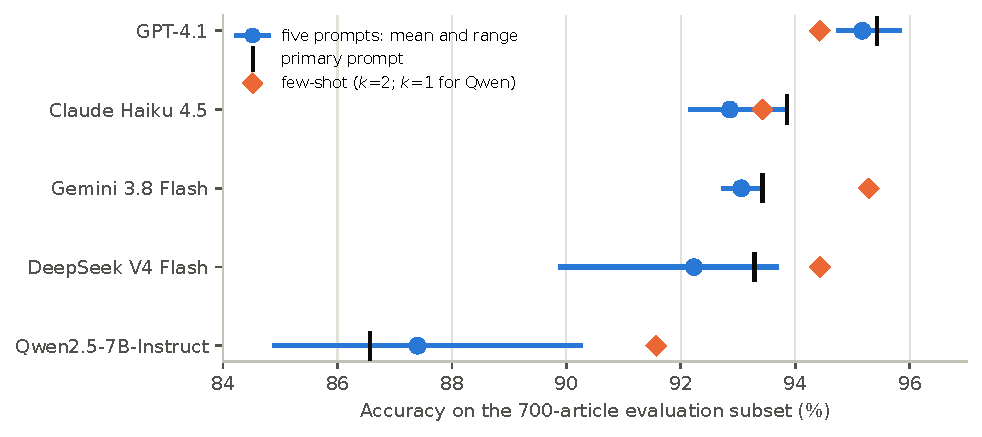
\includegraphics[width=0.85\textwidth]{fig_prompt_robustness.pdf}
\caption{Prompt sensitivity and few-shot effect on the 700-article evaluation subset. For each model: mean and range of zero-shot accuracy over five semantically equivalent prompts, the primary prompt, and the few-shot condition.}
\label{fig:prompts}
\end{figure}

\DIFadd{Table~\ref{tab:mapping} audits the label-mapping step over every run of each model. All four API models return a bare label for most requests, and the share of unmapped outputs on the full test set is 0.00\% (GPT-4.1), 0.04\% (Claude), 0.06\% (Gemini) and 0.01\% (DeepSeek), at most four articles. The resolved share shows which models deviate from the requested format and how: under one English prompt Claude Haiku 4.5 wrapped the label in surrounding text in 55\% of answers, under the Arabic prompts GPT-4.1 answered with the Arabic label name in 8--12\% of cases and Gemini added formatting to 97\% of answers; all of these were resolved by the fixed rules, }\DIFaddend and \DIFdelbegin \DIFdel{financial terminology. All }\DIFdelend \DIFaddbegin \DIFadd{none of them changed accuracy by more than the unmapped rate. Qwen2.5-7B }\DIFaddend zero-shot \DIFdelbegin \DIFdel{LLMs correctly identified the political/legal nature of the content through broader contextual understanding of court proceedings and governmental corruption cases }\DIFdelend \DIFaddbegin \DIFadd{produces 0.3--0.7\% unmapped outputs (a free continuation of the article instead of a label); after QLoRA the model answers with a bare label in every case. The mapping step is therefore not a hidden source of the differences reported above}\DIFaddend .

\DIFdelbegin \DIFdel{The second example shows how BERT can be confused by institutional overlap. The Emirates Green Building Council event about green innovations was misclassified as }\textit{\DIFdel{Medical}}%DIFAUXCMD
\DIFdel{, possibly due to associations between ``green'' terminology and health-related contexts in the training data. The LLMs' broader world knowledge allowed them to correctly associate green building technology with the }\textit{\DIFdel{Technology}} %DIFAUXCMD
\DIFdel{category. }\DIFdelend \DIFaddbegin \begin{table}[!ht]
\centering
\caption{Audit of the label-mapping step over all runs of each model (zero-shot prompts, few-shot, controls and repeats). ``Exact'' outputs are the bare label string; ``resolved'' outputs contained extra formatting, an Arabic label name, or a sentence with exactly one label and were mapped by the fixed rules; unmapped (no label, two labels, or an API error) outputs are scored as errors. Percentages of all outputs.}
\label{tab:mapping}
\small
\resizebox{\ifdim\width>\textwidth\textwidth\else\width\fi}{!}{%
\begin{tabular}{@{}l r r r r r r r@{}}
\toprule
\textbf{Model} & \textbf{Runs} & \textbf{Outputs} & \textbf{Exact (\%)} & \textbf{Resolved (\%)} & \textbf{Resolved, worst run (\%)} & \textbf{Unmapped (\%)} & \textbf{Unmapped, worst run (\%)} \\
\midrule
GPT-4.1 & 10 & 13,122 & 92.7 & 7.3 & 100.0 & 0.00 & 0.00 \\
Claude Haiku 4.5 & 10 & 13,122 & 97.0 & 3.0 & 55.4 & 0.02 & 0.04 \\
Gemini 3.8 Flash & 10 & 13,122 & 94.8 & 5.2 & 97.3 & 0.04 & 0.14 \\
DeepSeek V4 Flash & 10 & 24,844 & 99.9 & 0.1 & 0.6 & 0.02 & 0.07 \\
Qwen2.5-7B (zero-/few-shot) & 7 & 47,754 & 96.6 & 3.4 & 9.0 & 0.51 & 1.00 \\
Qwen2.5-7B + QLoRA (all) & 1 & 6,822 & 100.0 & 0.0 & 0.0 & 0.00 & 0.00 \\
\bottomrule
\end{tabular}}
\end{table}
\DIFaddend 


\DIFdelbegin \DIFdel{The third example reveals the }\textit{\DIFdel{Culture}}%DIFAUXCMD
\DIFdel{--}\textit{\DIFdel{Religion}} %DIFAUXCMD
\DIFdel{confusion in reverse. BERT misclassified a cultural article about Al Qasba Canal in Sharjah as }\textit{\DIFdel{Religion}}%DIFAUXCMD
\DIFdel{, while all LLMs correctly identified the cultural/leisure content. This suggests that certain cultural venue descriptions may share linguistic patterns with religious site descriptions in the training data.
}\DIFdelend \DIFaddbegin \subsection{\DIFadd{Controlled Analyses: Input Length and the Dateline}}
\label{sec:controls}
\DIFaddend 

\DIFdelbegin \subsubsection{\DIFdel{Model-Specific Error Patterns}}
%DIFAUXCMD
\addtocounter{subsubsection}{-1}%DIFAUXCMD
%DIFDELCMD < 

%DIFDELCMD < %%%
\DIFdel{Analysis of the 1}\DIFdelend \DIFaddbegin \DIFadd{Two interventions test whether either family relies on superficial cues. Input length: giving the frozen encoder 512 instead of 150 wordpieces adds 1.1 points on the full split and up to 5.9 points with 10 articles per class (Table~\ref{tab:lc}), so the lightweight systems do use the body of the article, not only its opening; restricting the LLMs to the first 100 words costs them 0.6--1.0 points (Table~\ref{tab:prompts}). Dateline: removing the city-and-source prefix from the test articles changes the dense head's accuracy from 96.4\% to 96.5\% ($\pm$0.2)}\DIFaddend , \DIFdelbegin \DIFdel{000-sample test set reveals systematic error patterns for each model architecture. Table~\ref{tab:error-summary} summarizes the key confusion patterns observed.
}%DIFDELCMD < 

%DIFDELCMD < \begin{table}[h!]
%DIFDELCMD <     \centering
%DIFDELCMD <     \caption{Summary of Model-Specific Error Patterns}
%DIFDELCMD <     \label{tab:error-summary}
%DIFDELCMD <     \small
%DIFDELCMD <     \begin{tabular}{lll}
%DIFDELCMD <         \toprule
%DIFDELCMD <         \textbf{Model} & \textbf{Primary Confusion} & \textbf{Likely Cause} \\
%DIFDELCMD <         \midrule
%DIFDELCMD <         BERT Dense Head & Finance $\leftrightarrow$ Tech & Numerical/financial terms in tech contexts \\
%DIFDELCMD <         & Religion $\leftrightarrow$ Culture & Shared formal MSA register \\
%DIFDELCMD <         \addlinespace
%DIFDELCMD <         GPT-4.1 & Tech $\rightarrow$ Finance & Economic framing of technology news \\
%DIFDELCMD <         & Religion $\rightarrow$ Culture & Historical/narrative style overlap \\
%DIFDELCMD <         \addlinespace
%DIFDELCMD <         Gemini-2.0-Flash & Tech $\rightarrow$ Finance & Business context dominance \\
%DIFDELCMD <         & Religion $\rightarrow$ Culture/Politics & Institutional announcement patterns \\
%DIFDELCMD <         \addlinespace
%DIFDELCMD <         Claude-3.5-Haiku & Religion $\rightarrow$ Culture (59\%) & Fundamental category boundary issues \\
%DIFDELCMD <         & Religion $\rightarrow$ Politics (28\%) & Religious-political discourse overlap \\
%DIFDELCMD <         \addlinespace
%DIFDELCMD <         DeepSeek V3 & Tech $\rightarrow$ Finance & Similar to GPT-4.1 patterns \\
%DIFDELCMD <         & Religion $\rightarrow$ Culture & Similar to GPT-4.1 patterns \\
%DIFDELCMD <         \bottomrule
%DIFDELCMD <     \end{tabular}
%DIFDELCMD < \end{table}
%DIFDELCMD < 

%DIFDELCMD < %%%
\DIFdel{Claude-3.5-Haiku exhibited the most severe category confusion, with 32 out of 135 Religion samples (24\% ) misclassified, primarily as }\textit{\DIFdel{Culture}} %DIFAUXCMD
\DIFdelend \DIFaddbegin \DIFadd{and removing it from training and test as well gives 96.4\% }\DIFaddend (\DIFdelbegin \DIFdel{59\% ) or }\textit{\DIFdel{Politics}} %DIFAUXCMD
\DIFdel{(28\%). This systematic failure suggests fundamental difficulties in distinguishing Gulf Arabic religious discourse from related cultural and political content without domain-specific training.
}%DIFDELCMD < 

%DIFDELCMD < %%%
\subsubsection{\DIFdel{Implications for Model Selection}}
%DIFAUXCMD
\addtocounter{subsubsection}{-1}%DIFAUXCMD
%DIFDELCMD < 

%DIFDELCMD < %%%
\DIFdel{These qualitative findings yield practical recommendations for Arabic news classification deployment:
}%DIFDELCMD < 

%DIFDELCMD < \begin{enumerate}
%DIFDELCMD <     \item %%%
\textbf{\DIFdel{High-stakes applications}}%DIFAUXCMD
\DIFdel{: Fine-tuned BERT models provide more consistent performance across all categories, particularly for Religion/Culture disambiguation where LLMs systematically struggle.
    }%DIFDELCMD < 

%DIFDELCMD <     \item %%%
\textbf{\DIFdel{Technology/Finance contexts}}%DIFAUXCMD
\DIFdel{: Consider ensemble approaches or post-hoc verification when articles contain both technological content and financial metrics, as both model families exhibit confusion in this domain.
    }%DIFDELCMD < 

%DIFDELCMD <     \item %%%
\textbf{\DIFdel{Resource-constrained scenarios}}%DIFAUXCMD
\DIFdel{: Among zero-shot LLMs, GPT-4.1 and DeepSeek V3 offer the best balance of performance and accessibility, while Claude-3.5-Haiku should be avoided for Arabic classification tasks without further prompt optimization}\DIFdelend \DIFaddbegin \DIFadd{$\pm$0.2); for the LLMs the change is between $-0.4$ and $+0.1$ points. Although the dateline is strongly correlated with the class in this corpus, neither family uses it as a shortcut, and the accuracy of the supervised systems does not depend on it}\DIFaddend .

\DIFdelbegin %DIFDELCMD < \item %%%
\textbf{\DIFdel{Edge cases}}%DIFAUXCMD
\DIFdel{: Articles with institutional announcements, historical narratives, or mixed domain terminology benefit from fine-tuned models that have learned corpus-specific classification conventions.
}%DIFDELCMD < \end{enumerate}
%DIFDELCMD < %%%
\DIFdelend \DIFaddbegin \subsection{\DIFadd{Training and Inference Cost}}
\label{sec:efficiency}
\DIFaddend 

\DIFdelbegin \DIFdel{These qualitative insights reinforce the quantitative findings: domain-specific }\DIFdelend \DIFaddbegin \DIFadd{Table~\ref{tab:timing} reports the measured cost of the supervised systems, and Table~\ref{tab:lora} the adaptation budget of the QLoRA baseline. The two frozen-encoder heads share one encoder pass over the corpus (60 seconds for 45,477 articles at 150 wordpieces, 111 seconds at 512, on an A100); once the embeddings exist, the dense head trains in 9 seconds and the SVM in 1.4 seconds, and both predict the 6,822 test articles in well under a second. Full }\DIFaddend fine-tuning \DIFdelbegin \DIFdel{enhances robustness, but different model heads exhibit distinct error profiles. Dense heads better capture semantic nuance,while SVM heads emphasize token-level features, leading to divergent failure cases.
}\DIFdelend \DIFaddbegin \DIFadd{takes 11.6 minutes on the full split and 15 seconds to predict the test set, and QLoRA of the 7B model 3.3 GPU-hours on the full split (0.3 GPU-hours with 100 articles per class). Zero-shot inference with the API models costs no training but one request per article at every use; at 2025--2026 list prices a single pass over the 6,822-article test set costs between about one and ten US dollars depending on the model, and the open-weight model served locally processed about ten articles per second on the same GPU. We do not report API latency because it is dominated by provider-side variability.
}\DIFaddend 

%DIF < %%%%%%%%%%%%%%%
\DIFaddbegin \begin{table}[!ht]
\centering
\caption{Training and inference cost of the supervised systems on one A100-PCIE-40GB (full training split of 31{,}833 articles; test split of 6{,}822). The frozen-encoder heads share one encoder pass, which dominates their cost and is reported separately; the head numbers are the training and prediction time of the head alone. Wall-clock seconds, mean over seeds.}
\label{tab:timing}
\small
\resizebox{\ifdim\width>\textwidth\textwidth\else\width\fi}{!}{%
\begin{tabular}{@{}l r r r@{}}
\toprule
\textbf{Component} & \textbf{Dense head} & \textbf{RBF-SVM (cuML)} & \textbf{Full fine-tuning} \\
\midrule
Encoder forward pass, all 45{,}477 articles (150 tokens) & \multicolumn{2}{c}{60} & -- \\
Encoder forward pass, all articles (512 tokens) & \multicolumn{2}{c}{111} & included \\
Training (150 tokens) & 8.8 & 1.4 & -- \\
Training (512 tokens) & 11.0 & 4.1 & 697 \\
Prediction on the test split (head only / full model) & 0.008 & 0.59 & 14.8 \\
\bottomrule
\end{tabular}}
\end{table}
\DIFaddend 

\DIFdelbegin \subsection{\DIFdel{Linguistic and Contextual Challenges for LLMs}}
%DIFAUXCMD
\addtocounter{subsection}{-1}%DIFAUXCMD
\DIFdelend \DIFaddbegin \begin{table}[!ht]
\centering
\caption{Adaptation budget of the QLoRA baseline (Qwen2.5-7B-Instruct, 4-bit NF4 base, LoRA rank 16, $\alpha=32$, all linear projections, 40.4\,M trainable parameters, 0.53\,\% of the 7.62\,B parameters of the base model; one NVIDIA A100-PCIE-40GB). Accuracy on the full test set.}
\label{tab:lora}
\small
\resizebox{\ifdim\width>\textwidth\textwidth\else\width\fi}{!}{%
\begin{tabular}{@{}l r r r r r r@{}}
\toprule
\textbf{Articles / class} & \textbf{Training articles} & \textbf{Epochs} & \textbf{Training tokens} & \textbf{GPU-hours} & \textbf{Peak VRAM (GB)} & \textbf{Accuracy (\%)} \\
\midrule
100 & 700 & 3 & 1.3\,M & 0.29 & 9.3 & 95.7 \\
1000 & 7,000 & 2 & 8.9\,M & 1.48 & 9.3 & 98.4 \\
all & 31,833 & 1 & 20.2\,M & 3.27 & 9.3 & 98.5 \\
\bottomrule
\end{tabular}}
\end{table}
\DIFaddend 


\DIFdelbegin \DIFdel{To strengthen the analysis, we examined the linguistic and contextual challenges faced by zero-shot LLMs in Arabic news classification, which help explain the performance gap compared to fine-tuned supervised approaches.
}%DIFDELCMD < 

%DIFDELCMD < %%%
\subsubsection{\DIFdel{Morphological Complexity and Tokenization}}
%DIFAUXCMD
\addtocounter{subsubsection}{-1}%DIFAUXCMD
%DIFDELCMD < 

%DIFDELCMD < %%%
\DIFdel{Arabic\'s rich morphological system presents unique challenges for general-purpose LLMs. Words in Arabic are formed through complex patterns of roots and affixes, with prefixes and suffixes that can encode grammatical information such as tense,gender, number, and case. For instance, a single Arabic word can contain a conjunction, future tense marker, verb root, plural masculine suffix, and object pronoun---all in a single token. General-purpose LLMs trained primarily on English and other European languages may struggle with such dense morphological encoding, leading to suboptimal semantic understanding.
}%DIFDELCMD < 

%DIFDELCMD < %%%
\DIFdel{In contrast, CAMeLBERT was pre-trained on 167 GB of Arabic text using domain-adaptive tokenization strategies that better capture morphological boundaries. The fine-tuning process further specializes these representations for news categorization, allowing the model to distinguish subtle morphological patterns that signal topical boundaries. For example, technical terminology in }\textit{\DIFdel{Technology}} %DIFAUXCMD
\DIFdel{articles often follows specific derivational patterns that fine-tuned models learn to associate with the correct category.
}%DIFDELCMD < 

%DIFDELCMD < %%%
\subsubsection{\DIFdel{Diglossia and Register Variation}}
%DIFAUXCMD
\addtocounter{subsubsection}{-1}%DIFAUXCMD
%DIFDELCMD < 

%DIFDELCMD < %%%
\DIFdel{Arabic exists in a state of diglossia, with Modern Standard Arabic (MSA)used in formal writing and various dialects in spoken communication. News articles predominantly useMSA,but they may incorporate dialectal expressions, loanwords, or code-switching, particularly in quotes or informal sections. Zero-shot LLMs, lacking exposure to the specific stylistic conventions of Gulf Arabic news sources, may misinterpret these register shifts as topical indicators rather than stylistic choices. }%DIFDELCMD < 

%DIFDELCMD < %%%
\DIFdel{The misclassification of medical content as }\textit{\DIFdel{Religion}} %DIFAUXCMD
\DIFdel{(Table~\ref{tab:model-evaluation}) exemplifies this challenge. Both domains share formal register and may use similar syntactic structures for institutional announcements. Without fine-tuning on domain-specific examples , LLMs may over-weight superficial lexical similarities (e.g., honorific titles, formal verb forms) at the expense of semantic content. Fine-tuned models, having seen numerous examples from each category, develop robust feature representations that distinguish genuine religious content from other formal discourse}\DIFdelend \DIFaddbegin \subsection{\DIFadd{Qualitative Error Analysis}}
\label{sec:qualitative}

\DIFadd{The examples below are drawn from the final runs on the shared test split (dense head, seed 0; API models with the primary prompt). Table~\ref{tab:correct-examples} shows articles that every system classifies correctly: unambiguous domain vocabulary (a poetry evening, a football club presidency, console sales figures) that needs no corpus-specific knowledge}\DIFaddend .

\DIFdelbegin \subsubsection{\DIFdel{Named Entity Ambiguity and Cultural Context}}
%DIFAUXCMD
\addtocounter{subsubsection}{-1}%DIFAUXCMD
\DIFdelend \DIFaddbegin \begin{table}[h!]
    \centering
    \caption{Articles classified correctly by the dense head and by all four API LLMs.}
    \label{tab:correct-examples}
    \small
    \begin{tabularx}{\textwidth}{>{\raggedleft\arraybackslash}p{0.62\textwidth} c c}
        \toprule
        \textbf{Text (excerpt)} & \textbf{Category} & \textbf{All systems} \\
        \midrule
        \RTL{ينظم بيت الشعر في الشارقة عند السابعة والنصف من مساء اليوم أمسية يحييها الشاعر حامد الحرباوي والشاعر عمر عبدالحكيم بكور ويقدم للأمسية الشاعر عبدالرزاق الدرباس.} & Culture & \checkmark \\
        \addlinespace
        \RTL{سيبقى فلورنتينو بيريز رئيساً لنادي ريال مدريد الإسباني حتى 2017 لعدم وجود أي مرشح غيره للانتخابات المقررة في وقت لاحق من الشهر الجاري.} & Sports & \checkmark \\
        \addlinespace
        \RTL{أعلنت مايكروسوفت أمس أن مبيعات منصة إكس بوكس 360 تجاوزت 30 مليوناً في العالم، مسجلة بذلك نمواً قياسياً بنسبة 28\% على العام الماضي.} & Tech & \checkmark \\
        \bottomrule
    \end{tabularx}
\end{table}
\DIFaddend 

\DIFdelbegin \DIFdel{Arabic news articles frequently reference named entities---organizations, locations, public figures---whose categorization depends heavily on cultural and contextual knowledge. For example, Al-Hilal could refer to a prominent football club (}\DIFdelend \DIFaddbegin \DIFadd{Table~\ref{tab:bert-correct-llm-wrong} shows articles that the supervised head classifies correctly and most LLMs do not. All three are cases where the publisher's section assignment follows the }\emph{\DIFadd{institution}} \DIFadd{behind the story rather than its }\emph{\DIFadd{topic}}\DIFadd{: a reading-month campaign organised by the Ministry of Health is filed under }\textit{\DIFadd{Medical}} \DIFadd{(all four LLMs: }\DIFaddend \textit{\DIFdelbegin \DIFdel{Sports}\DIFdelend \DIFaddbegin \DIFadd{Culture}\DIFaddend })\DIFdelbegin \DIFdel{or the Red Crescent humanitarian organization (}\DIFdelend \DIFaddbegin \DIFadd{; the expulsion of a missionary by the Mauritanian authorities is filed under }\textit{\DIFadd{Politics}} \DIFadd{(all four: }\DIFaddend \textit{\DIFdelbegin \DIFdel{Politics or Society}\DIFdelend \DIFaddbegin \DIFadd{Religion}\DIFaddend })\DIFdelbegin \DIFdel{. Similarly, Al-Nassr is both a sports club and a common term meaning victory used across domains.
}%DIFDELCMD < 

%DIFDELCMD < %%%
\DIFdel{Zero-shot LLMs, despite their broad knowledge, may lack the fine-grained understanding of Gulf region entities and their primary associations within this specific news corpus. The complete failure of Claude-3.5-Haiku on the }\textit{\DIFdel{Religion}} %DIFAUXCMD
\DIFdel{category (0\% recall) suggests systematic misunderstanding of how religious topics are framed in Gulf Arabic journalism. This contrasts sharply with fine-tuned models, which learn }\DIFdelend \DIFaddbegin \DIFadd{; and a health-insurance company's smartphone applications are filed under }\textit{\DIFadd{Medical}} \DIFadd{(three LLMs: }\textit{\DIFadd{Tech}}\DIFadd{). The LLM answers are defensible readings of the text; the supervised systems have learned the publisher's convention from thousands of labelled examples, which is precisely the advantage of in-domain supervision and also a reminder that part of the measured gap reflects }\DIFaddend corpus-specific \DIFdelbegin \DIFdel{entity-category associations during training. The supervised learning process effectively builds a domain-specific knowledge graph that captures which entities and phrases reliably predict each news category}\DIFdelend \DIFaddbegin \DIFadd{labelling rather than language understanding}\DIFaddend .

\DIFdelbegin \subsubsection{\DIFdel{Prompt Engineering Limitations}}
%DIFAUXCMD
\addtocounter{subsubsection}{-1}%DIFAUXCMD
\DIFdelend \DIFaddbegin \begin{table}[h!]
    \centering
    \caption{Articles classified correctly by the dense head and incorrectly by most zero-shot LLMs.}
    \label{tab:bert-correct-llm-wrong}
    \small
    \begin{tabularx}{\textwidth}{@{}>{\raggedleft\arraybackslash}X c c >{\raggedright\arraybackslash}p{0.26\textwidth}@{}}
        \toprule
        \textbf{Text (excerpt)} & \textbf{True label} & \textbf{Dense head} & \textbf{LLM predictions} \\
        \midrule
        \RTL{دبي: «الخليج» أقامت وزارة الصحة ووقاية المجتمع حفل إطلاق فعاليات شهر القراءة لعام 2018 تحت شعار «الإمارات تقرأ الإمارات ترقى» في ديوان الوزارة بدبي، وأعلنت الوزارة عن برنامجها الكامل لشهر القراءة الذي يتضمن 117 فعالية في عدد من المستشفيات والمراكز الصحية.} &
        Medical & Medical \checkmark & GPT-4.1: Culture \texttimes \newline Claude: Culture \texttimes \newline Gemini: Culture \texttimes \newline DeepSeek: Culture \texttimes \\
        \addlinespace[1em]
        \RTL{أبعدت السلطات الموريتانية مبشرة نرويجية من الأراضي الموريتانية بعد توقيفها وهي تمارس نشاطات تبشيرية في ولاية آدرار شمال العاصمة نواكشوط.} &
        Politics & Politics \checkmark & GPT-4.1: Religion \texttimes \newline Claude: Religion \texttimes \newline Gemini: Religion \texttimes \newline DeepSeek: Religion \texttimes \\
        \addlinespace[1em]
        \RTL{أبوظبي: «الخليج» أعلنت الشركة الوطنية للضمان الصحي - ضمان أمس عن إطلاق تطبيقين إلكترونيين، أحدهما لمشتركي «ضمان» والآخر لمشتركي «ثقة» على الأجهزة الذكية.} &
        Medical & Medical \checkmark & GPT-4.1: Tech \texttimes \newline Claude: Tech \texttimes \newline Gemini: Tech \texttimes \newline DeepSeek: Finance \texttimes \\
        \bottomrule
    \end{tabularx}
\end{table}
\DIFaddend 

\DIFdelbegin \DIFdel{The performance of zero-shot LLMs is highly sensitive to prompt design, yet optimal prompts for Arabic classification may differ significantly from English best practices due to structural and pragmatic differences between the languages. Arabic\'s VSO (Verb-Subject-Object) word order flexibility and optional casemarking create ambiguities that English prompts may not adequately address. Furthermore, culturally appropriate framing of classification instructions requires understanding how category boundaries are conceptualized in Arabic journalism---for instance, where the line between }\textit{\DIFdel{Politics}} %DIFAUXCMD
\DIFdel{and }\DIFdelend \DIFaddbegin \DIFadd{Table~\ref{tab:llm-correct-bert-wrong} shows the reverse case. A tender for the construction of a new trade-centre building was labelled }\textit{\DIFadd{Tech}} \DIFadd{by the head and }\DIFaddend \textit{\DIFdelbegin \DIFdel{Religion}\DIFdelend \DIFaddbegin \DIFadd{Finance}\DIFaddend } \DIFdelbegin \DIFdel{falls in coverage of religious authorities making policy statements.
}\DIFdelend \DIFaddbegin \DIFadd{by every LLM, and a food-control authority's new inspection systems were labelled }\textit{\DIFadd{Medical}} \DIFadd{by the head and }\textit{\DIFadd{Tech}} \DIFadd{by every LLM; in both the head appears to key on domain vocabulary (construction and office space; food safety and inspection) that co-occurs with the wrong class in the training data, while the LLMs read the article as a whole.
}\DIFaddend 

\DIFdelbegin \DIFdel{Without extensive prompt optimization for each LLM}\DIFdelend \DIFaddbegin \begin{table}[h!]
    \centering
    \caption{Articles classified correctly by all four zero-shot LLMs and incorrectly by the dense head.}
    \label{tab:llm-correct-bert-wrong}
    \small
    \begin{tabularx}{\textwidth}{@{}>{\raggedleft\arraybackslash}X c c >{\raggedright\arraybackslash}p{0.26\textwidth}@{}}
        \toprule
        \textbf{Text (excerpt)} & \textbf{True label} & \textbf{Dense head} & \textbf{LLM predictions} \\
        \midrule
        \RTL{مددت شركة مركز دبي التجاري العالمي الموعد النهائي لمناقصة عقد إنشاء المرحلة الأولى من المركز الجديد حتى 27 نوفمبر الجاري بدلاً من 13 منه، وتشمل المرحلة الأولى إنشاء 90 ألف متر من المكاتب فضلاً عن 555 غرفة فندقية.} &
        Finance & Tech \texttimes & GPT-4.1: Finance \checkmark \newline Claude: Finance \checkmark \newline Gemini: Finance \checkmark \newline DeepSeek: Finance \checkmark \\
        \addlinespace[1em]
        \RTL{كشف جهاز أبوظبي للرقابة الغذائية عن 5 أنظمة مبتكرة في مجال الرقابة الغذائية وخدمة المتعاملين، يسعى الجهاز من خلالها إلى التفعيل الأمثل للدور الرقابي في مجال الزراعة وسلامة الغذاء.} &
        Tech & Medical \texttimes & GPT-4.1: Tech \checkmark \newline Claude: Tech \checkmark \newline Gemini: Tech \checkmark \newline DeepSeek: Tech \checkmark \\
        \bottomrule
    \end{tabularx}
\end{table}

\DIFadd{Across the test split the error profiles summarised in Table~\ref{tab:error-summary} are stable across prompts and models: the supervised systems confuse }\textit{\DIFadd{Religion}} \DIFadd{with }\textit{\DIFadd{Culture}} \DIFaddend and \DIFdelbegin \DIFdel{careful validation on Arabic-specific test cases, }\DIFdelend \DIFaddbegin \textit{\DIFadd{Tech}} \DIFadd{with }\textit{\DIFadd{Finance}} \DIFadd{in both directions, at a rate of a few percent; the }\DIFaddend zero-shot \DIFdelbegin \DIFdel{performance remains inconsistent. The 18-percentage-point gap between GPT-4.1 (93\%) and Claude-3.5-Haiku (75\%) suggests that model architecture, training datacomposition, }\DIFdelend \DIFaddbegin \DIFadd{LLMs share these two confusions, add }\textit{\DIFadd{Medical}}\DIFadd{$\to$}\textit{\DIFadd{Culture}}\DIFadd{/}\textit{\DIFadd{Tech}} \DIFaddend and \DIFdelbegin \DIFdel{inference-time prompt processing all significantly impact Arabic text understanding.
Fine-tuned modelsbypass these challenges entirely, as the classification headlearns optimal decision boundaries directly from labeled examples without relying on natural language instructions}\DIFdelend \DIFaddbegin \textit{\DIFadd{Politics}}\DIFadd{$\to$}\textit{\DIFadd{Religion}}\DIFadd{, and their }\textit{\DIFadd{Religion}}\DIFadd{$\to$}\textit{\DIFadd{Culture}} \DIFadd{rate is about four times that of the supervised head}\DIFaddend .

\DIFdelbegin \subsubsection{\DIFdel{Advantages of Supervised Fine-Tuning}}
%DIFAUXCMD
\addtocounter{subsubsection}{-1}%DIFAUXCMD
\DIFdelend \DIFaddbegin \begin{table}[h!]
    \centering
    \caption{Largest confusions on the shared test split (counts out of 973--975 articles per true class).}
    \label{tab:error-summary}
    \small
    \begin{tabular}{llr}
        \toprule
        \textbf{System} & \textbf{Confusion} & \textbf{Count} \\
        \midrule
        Dense head (150 tokens) & Religion $\to$ Culture & 44 \\
        & Tech $\to$ Finance & 28 \\
        & Culture $\to$ Religion & 20 \\
        \addlinespace
        GPT-4.1 (zero-shot) & Religion $\to$ Culture & 172 \\
        & Religion $\to$ Medical & 34 \\
        & Tech $\to$ Finance & 32 \\
        & Politics $\to$ Religion & 28 \\
        & Medical $\to$ Culture & 23 \\
        \bottomrule
    \end{tabular}
\end{table}
\DIFaddend 

\DIFdelbegin \DIFdel{The consistent 97\% accuracy achieved by both BERT-based architectures demonstrates the effectiveness of supervised fine-tuning in overcoming the above challenges. Several mechanisms contribute to this success:
}%DIFDELCMD < 

%DIFDELCMD < \begin{itemize}
%DIFDELCMD <     \item %%%
\textbf{\DIFdel{Task-specific feature learning}}%DIFAUXCMD
\DIFdel{: Fine-tuning adjusts the entire model to emphasize features relevant to news categorization, down-weighting irrelevant linguistic patterns that dominate pre-training objectives. }%DIFDELCMD < 

%DIFDELCMD <     \item %%%
\textbf{\DIFdel{Boundary refinement}}%DIFAUXCMD
\DIFdel{: Exposure to labeled examples from all categories allows the model to learn precise decision boundaries that separate similar domains (e.g., }\textit{\DIFdel{Technology}} %DIFAUXCMD
\DIFdel{vs. }\textit{\DIFdel{Finance}} %DIFAUXCMD
\DIFdel{in business contexts).
    }%DIFDELCMD < 

%DIFDELCMD <     \item %%%
\textbf{\DIFdel{Error correction feedback}}%DIFAUXCMD
\DIFdel{: The backpropagation of classification errors during training directly updates model parameters to reduce confusion between frequently conflated categories, creating category-specific feature detectors}\DIFdelend \DIFaddbegin \section{\DIFadd{Discussion}}
\label{discussion}

\DIFadd{The results answer a narrower question than the one posed in an earlier version of this work, and they answer it more reliably. The question is not whether lightweight models are better than large language models, but how much in-domain supervision it takes, and in which form, to beat zero-shot and few-shot inference on a well-defined Arabic classification task, and what each option costs}\DIFaddend .

\DIFdelbegin %DIFDELCMD < \item %%%
\textbf{\DIFdel{Calibrated confidence}}%DIFAUXCMD
\DIFdel{: Fine-tuned models produce well-calibrated probability distributions over categories, reflecting genuine uncertainty in ambiguous cases rather than the overconfident or poorly calibrated predictions sometimes observed in }\DIFdelend \DIFaddbegin \DIFadd{First, a frozen Arabic encoder with a small trained decision function is a strong system for this task: 96--98\% accuracy on a deduplicated test split, three to five points above the best }\DIFaddend zero-shot \DIFdelbegin \DIFdel{scenarios. }%DIFDELCMD < \end{itemize}
%DIFDELCMD < 

%DIFDELCMD < %%%
\DIFdel{The near-identical performance of Dense and SVM heads (both 97\%) further validates that the primary performance gains come from the fine-tuned BERT encoder rather than the classification architecture. This suggests that domainadaptation at the representation level---learning Arabic news-specific semantic embeddings---is the critical factor for high accuracy. }%DIFDELCMD < 

%DIFDELCMD < %%%
\DIFdel{These qualitative insights reinforce the quantitative findings: while large language models demonstrate impressive general capabilities, domain-specific }\DIFdelend \DIFaddbegin \DIFadd{LLM on the same articles, with statistical significance that leaves no doubt. The gain does not come from adapting the encoder to the domain, because the encoder is not adapted; it comes from supervised decision-boundary learning on a representation that already separates the classes well. When the encoder is adapted, by full }\DIFaddend fine-tuning \DIFdelbegin \DIFdel{remains essential for achieving robust performance on Arabic NLP tasks. The linguistic complexity, cultural specificity, and morphological richness of Arabic create barriers that general-purpose models struggle to overcome through }\DIFdelend \DIFaddbegin \DIFadd{or by QLoRA on a 7B instruction-tuned model, another two to three points follow, and the two adapted systems converge to the same ceiling (98.5--98.9\%). The learning curve places the crossover with }\DIFaddend zero-shot \DIFdelbegin \DIFdel{inference alone, even with sophisticated prompting strategies. }%DIFDELCMD < 

%DIFDELCMD < %%%
\section{\DIFdel{Discussion}}
%DIFAUXCMD
\addtocounter{section}{-1}%DIFAUXCMD
%DIFDELCMD < \label{discussion}
%DIFDELCMD < 

%DIFDELCMD < %%%
\DIFdel{The results highlight several important insights into the relative strengths and weaknesses of domain-adapted supervised models versus general-purpose zero-shot }\DIFdelend LLMs \DIFdelbegin \DIFdel{in Arabic text classification}\DIFdelend \DIFaddbegin \DIFadd{at about 100 labelled articles per class, and with the best few-shot condition at about 500 per class}\DIFaddend .

\DIFdelbegin \DIFdel{First, the domain-specific supervised models---particularly the BERT-based Dense Head and SVM Head---consistently outperformed }\DIFdelend \DIFaddbegin \DIFadd{Second, the }\DIFaddend zero-shot LLMs \DIFdelbegin \DIFdel{across all evaluation metrics. The fine-tuned models captured task-specific linguistic and morphological cues in Arabic that generalist models overlooked. For instance, in the }\textit{\DIFdel{Politics}} %DIFAUXCMD
\DIFdelend \DIFaddbegin \DIFadd{are far more consistent with each other than the earlier version of this study suggested. Four API models from four providers lie within 1.3 points, their ranking is stable across five prompts in two languages, }\DIFaddend and \DIFdelbegin \textit{\DIFdel{Finance}} %DIFAUXCMD
\DIFdel{categories, fine-tuned models effectively recognized subtle lexical markers, collocations, and syntactic structures that carry domain-specific meaning. Zero-shot LLMs, trained on broad multilingual corpora, tended to conflate semantically close but contextually distinct terms, leading to lower precision in these categories. This demonstrates the value of explicit adaptation to domain distributions where word choice and framing strongly influence meaning.
}\DIFdelend \DIFaddbegin \DIFadd{decoding at temperature 0 is reproducible. Their accuracy is nevertheless bounded by two things that in-context examples cannot fix: a class, }\textit{\DIFadd{Religion}}\DIFadd{, whose boundary with }\textit{\DIFadd{Culture}} \DIFadd{follows the publisher's section conventions rather than the surface topic, and a handful of institution-based labelling conventions illustrated in Section~\ref{sec:qualitative}. Few-shot examples help the weaker models by one to five points and the stronger models not at all, which suggests that the stronger models already understand the task and lack the convention, not the instruction. The 7B open-weight model is the clearest illustration: 85\% zero-shot, 90\% with one example per class, 96\% with QLoRA on 100 articles per class and 98.5\% with the full split.
}\DIFaddend 

\DIFdelbegin \DIFdel{Second, the analysis reveals a clear asymmetry in the performance of }\DIFdelend \DIFaddbegin \DIFadd{Third, the controlled analyses argue against two explanations that we had entertained and that the reviewers of the earlier version rightly questioned. Neither family uses the newspaper dateline, a highly class-correlated prefix, as a shortcut; and both families use more than the opening words of an article. We therefore make no claim about the internal mechanisms of either family. What the data support is a statement about supervision: the information that separates the supervised systems from }\DIFaddend zero-shot \DIFdelbegin \DIFdel{LLMs across different categories. These models performed relatively better in more objective or factual domains such as }\textit{\DIFdel{Technology}} %DIFAUXCMD
\DIFdel{or }\textit{\DIFdel{Sports}}%DIFAUXCMD
\DIFdel{, where classboundaries rely on surface-level lexical cues and globally shared terminology.
However, they struggled in subjective or culturally sensitive categories such as }\textit{\DIFdel{Religion}}%DIFAUXCMD
\DIFdel{, where accurate classification requires nuanced understanding of culturally embedded references and pragmatic context. Notably, Claude 3.5-Haiku failed to classify any instance in the }\textit{\DIFdel{Religion}} %DIFAUXCMD
\DIFdel{class. This failure suggests that the model\'s training data or alignment constraints may lead to systematic avoidance or misclassification of religion-related content, possibly due to safety filters, data gaps, or alignment bias against sensitive domains. By contrast, the fine-tuned models, trained directly on representative labeled data , learned to reliably separate culturally salient linguistic patterns that general-purpose systems avoided.
}\DIFdelend \DIFaddbegin \DIFadd{inference on this corpus is carried by the labels, and most of it is available from a few hundred labelled articles per class.
}\DIFaddend 

\DIFdelbegin \DIFdel{Third, we observe trade-offs in computational efficiency. The SVM Head trained more quickly than the Dense Head (4.38 vs.\ 10.54 seconds), making it more suitable when rapid retraining or limited compute resources are key constraints.
However, the Dense Head delivered slightly faster inference, which is advantageous for latency-sensitive applications such as interactive systems . These results show that model choice should depend on deployment requirements rather than absolute performance alone.
}\DIFdelend \DIFaddbegin \DIFadd{Fourth, the cost picture favours the lightweight systems whenever labels exist. One encoder pass of a minute, a head that trains in seconds, sub-second prediction of the whole test set, no per-request fee and no dependence on a third-party service; full fine-tuning adds twelve minutes of GPU time, and QLoRA of a 7B model about three GPU-hours. Zero-shot inference requires no labels and no training, which remains decisive when labels are unavailable or the label set changes often, but it costs a request per article at every use and its behaviour depends on the provider's snapshot, three of which were retired within the year this work was revised.
}\DIFaddend 

\DIFdelbegin \DIFdel{Beyond accuracy and efficiency, supervised models also offered predictability and control. API-based LLMs exhibit runtime variability due to external serviceconditions, while fine-tuned models provided stable inference times and full transparency in training and deployment. This consistency is critical in real-world pipelines where reproducibility and predictable costs are essential.
}%DIFDELCMD < 

%DIFDELCMD < %%%
\DIFdel{Taken together, the findings suggest several directions for future research. One promising line is domain-adaptive pretraining for LLMs on Arabic corpora, which could bridge the gap between generalization and cultural grounding. Another is exploring }\DIFdelend \DIFaddbegin \paragraph{\DIFadd{Limitations.}} \DIFadd{The study covers one publisher, one language variety (Modern Standard Arabic) and a label set whose boundaries partly reflect editorial conventions; the size of the crossover will differ on noisier or dialectal corpora. The prompt-robustness, }\DIFaddend few-shot \DIFdelbegin \DIFdel{prompting strategies, which may enhance zero-shot models without full retraining. Finally, extending evaluation to dialectal Arabic corpora would test }\DIFdelend \DIFaddbegin \DIFadd{and control analyses use a fixed 700-article subset on which the LLMs score 1.4--2.6 points higher than on the full test set; subset results are therefore reported as within-subset differences, and the main comparison and }\DIFaddend the \DIFdelbegin \DIFdel{robustness of both supervised and zero-shot approaches in more linguistically diverse and realistic settings. Such directions would contribute to building hybrid systems that combine the scalability of large pretrained models with the adaptability of lightweight fine-tuning. }%DIFDELCMD < 

%DIFDELCMD < %%%
\DIFdel{In summary, supervised domain-adapted models remain the most effective solution for high-accuracy Arabic text classification under current conditions. However, strategically combining them with foundation models —through domain adaptation, few-shot learning, or dialectal transfer—represents a compelling future path for both research and deployment}\DIFdelend \DIFaddbegin \DIFadd{learning curve use the full split. The adapted-LLM baseline uses one open-weight model and one LoRA configuration, and full fine-tuning on the full split uses a single seed. API models were evaluated through a routing service with pinned providers; the identifiers served are logged, but the behaviour of hosted models may change when providers update them. Finally, one of the API models (Gemini 3.8 Flash) could not be run with reasoning fully disabled and used a minimal reasoning budget, which we report but cannot remove}\DIFaddend .

\section{Conclusion}
\label{conclusion}

This \DIFdelbegin \DIFdel{study benchmarked lightweight supervised models against state-of-the-art zero-shot LLMs for Arabic multi-class text classification using the balanced SANAD (AlKhaleej) dataset. Two architectures based on CAMeLBERT embeddings—a dense neural head and an SVM classifier—were compared to leading LLMs: GPT-4.1, DeepSeek V3, Gemini 2.0-Flash, and Claude 3.5-Haiku. }%DIFDELCMD < 

%DIFDELCMD < %%%
\DIFdel{The fine-tuned supervised models consistently outperformed their zero-shot counterparts across all evaluation metrics. Both the Dense and SVM heads achieved 97}\DIFdelend \DIFaddbegin \DIFadd{paper compared lightweight supervised classifiers built on a frozen CAMeLBERT encoder with large language models for seven-way Arabic news classification on the SANAD-AlKhaleej corpus, under a protocol in which every system is scored on the same deduplicated test split, LLM decoding is deterministic, prompt sensitivity and output parsing are measured, and the amount of supervision is varied on both sides. With the full training split the frozen-encoder heads reach 96.4--98.1}\DIFaddend \% accuracy, \DIFdelbegin \DIFdel{while the best-performing LLM (}\DIFdelend \DIFaddbegin \DIFadd{full fine-tuning 98.9\%, and a QLoRA-adapted Qwen2.5-7B-Instruct 98.5\%, against 91.5--92.8\% for zero-shot }\DIFaddend GPT-4.1\DIFdelbegin \DIFdel{) reached 93\%. Claude 3.5-Haiku lagged significantly, particularly in sensitive categories such as }\DIFdelend \DIFaddbegin \DIFadd{, Claude Haiku 4.5, Gemini 3.8 Flash and DeepSeek V4 Flash, all of which share a weakness on the }\DIFaddend \textit{Religion} \DIFaddbegin \DIFadd{class. About 100 labelled articles per class suffice for a 0.3\,M-parameter head to match the best zero-shot LLM, and 500 per class for the 512-wordpiece head to pass the best few-shot condition on the same articles; prompt wording moves the strong API models by less than one point, replicate runs are identical, and neither the dateline nor the opening words of an article act as a shortcut for any system}\DIFaddend .
\DIFdelbegin \DIFdel{Class-level analysis further confirmed the robustness of fine-tuned models , especially in capturing nuanced semantic distinctions.
}\DIFdelend 

\DIFdelbegin \DIFdel{Efficiency evaluation showed that the SVM Head trains faster, while the Dense Head offers slightly better inference speed. In contrast}\DIFdelend \DIFaddbegin \DIFadd{The practical recommendation is therefore conditional on labels. With a few hundred labelled articles per class, a frozen Arabic encoder and a small head give the best accuracy per unit of cost, and fine-tuning or parameter-efficient adaptation of a larger model buys the last two to three points; without labels}\DIFaddend , zero-shot LLMs \DIFdelbegin \DIFdel{, though capable of generalization, exhibited variable latency and reduced reliability in culturally specific contexts without task adaptation}\DIFdelend \DIFaddbegin \DIFadd{are a reasonable option at 91--93\% whose main failure mode is predictable and class-specific. Future work should extend the protocol to dialectal and multi-publisher corpora, where editorial conventions are less uniform, and examine whether the label conventions that separate the two families can be conveyed to LLMs through instructions rather than examples}\DIFaddend .

\DIFdelbegin \DIFdel{In conclusion, domain-specific fine-tuned models remain the most reliable and efficient option for Arabic text classification in practical settings. They offer strong performance, consistent behavior, and operational flexibility. Future research should investigate hybrid approaches—such as prompt-tuning or model distillation—that combine the generalization strengths of LLMs with the efficiency and controllability of supervised architectures, particularly for deployment inlow-resource or latency-sensitive environments. }\DIFdelend \DIFaddbegin \section*{\DIFadd{Data and code availability}}
\DIFadd{The split file with per-article checksums, the deduplication clusters, the evaluation subset, all per-article predictions and raw LLM outputs, the QLoRA adaptation budgets and the complete code are available at }\url{https://github.com/omaratef3221/Bert-rbf-arabic-text-classification} \DIFadd{(folder }\texttt{\DIFadd{revision/}}\DIFadd{). The SANAD corpus is available from its authors \mbox{%DIFAUXCMD
\cite{elnagar2020arabic}}\hskip0pt%DIFAUXCMD
.
}\DIFaddend 

\DIFaddbegin \appendix
\section{\DIFadd{Prompt variants}}
\label{app:prompts}

\DIFadd{All prompts present the seven labels and request exactly one. }\texttt{[\DIFadd{examples}]} \DIFadd{is empty in the zero-shot condition; in the few-shot conditions it holds $k$ exemplars per class in the form ``Text: \ldots\ Class: \ldots''. The label list is }\texttt{[\DIFadd{'Culture', 'Finance', 'Medical', 'Politics', 'Religion', 'Sports', 'Tech'}]}\DIFadd{; in the Arabic prompts each label is followed by its Arabic gloss.
}

\begin{description}[leftmargin=1.2cm,style=nextline]
\item[\texttt{\DIFadd{en\_v1}} \DIFadd{(original wording)}] \DIFadd{Act as an Arabic Text Classifier that has to classify between the following: }[\DIFadd{labels}]\DIFadd{. Write only the final output class without anything more. }[\DIFadd{examples}] \DIFadd{Text: }[\DIFadd{text}] \DIFadd{Class:
}\item[\texttt{\DIFadd{en\_v2}} \DIFadd{(primary)}] \textit{\DIFadd{System:}} \DIFadd{You are a precise news-topic classifier for Modern Standard Arabic. }\textit{\DIFadd{User:}} \DIFadd{Classify the Arabic news article below into exactly one of these categories: }[\DIFadd{labels}]\DIFadd{. Respond with the category name only, copied exactly from the list, with no explanation. }[\DIFadd{examples}] \DIFadd{Article: }[\DIFadd{text}] \DIFadd{Category:
}\item[\texttt{\DIFadd{en\_v3}}] \DIFadd{Which section of a Gulf Arabic newspaper would the following article appear in? Choose one of: }[\DIFadd{labels}]\DIFadd{. }[\DIFadd{examples}] \DIFadd{Article: }[\DIFadd{text}] \DIFadd{Answer with one word from the list:
}\item[\texttt{\DIFadd{ar\_v1}}] \RTL{تصرّف كمصنّف نصوص عربية. صنّف المقال التالي إلى واحدة فقط من الفئات التالية: [labels] اكتب اسم الفئة فقط كما هو مكتوب في القائمة دون أي إضافة. [examples] المقال: [text] الفئة:}
\item[\texttt{\DIFadd{ar\_v2}}] \textit{\DIFadd{System:}} \RTL{أنت مصنّف دقيق لموضوعات الأخبار المكتوبة بالعربية الفصحى.} \textit{\DIFadd{User:}} \RTL{حدّد القسم الصحفي الذي ينتمي إليه المقال التالي. الأقسام المتاحة هي: [labels] أجب بكلمة واحدة فقط من القائمة أعلاه. [examples] المقال: [text] القسم:}
\end{description}

\DIFaddend \bibliographystyle{elsarticle-harv}
%DIF < \bibliographystyle{model5-names}\biboptions{authoryear}
\bibliography{references,references_revision}

\end{document}
